

\dominitoc
\tableofcontents

%\emptypage
\newpage

\chapternonum{Introduction}

%
% There are worlds out there where the sky is burning, and the sea’s asleep, and the rivers dream;
% people made of smoke and cities made of song. Somewhere there’s danger, somewhere there’s injustice,
% and somewhere else the tea’s getting cold. Come on, Ace. We’ve got work to do.”
%
% It’s like when you’re a kid. The first time they tell you that the world’s turning and you just can’t
% quite believe it ’cause everything looks like it’s standing still… I can feel it: the turn of the Earth.
% The ground beneath our feet is spinning at 1,000 miles an hour and the entire planet is hurtling around
% the sun at 67,000 miles an hour, and I can feel it. We’re falling through space, you and me, clinging to
% the skin of this tiny little world, and if we let go… That’s who I am.
%
% The universe is big. It’s vast and complicated and ridiculous. And sometimes, very rarely, impossible
% things just happen and we call them miracles.
%
% So, you find a breach, probe it, the sphere comes through, 600 feet above London, BAM! It leaves a hole
% in the fabric of reality. And that hole, you think: “Should we leave it alone, should we back off, should
% we play it safe?” NAH, you think: “Let’s make it BIGGER!”
%
% People assume that time is a strict progression of cause to effect, but actually from a non-linear,
% non-subjective viewpoint, it’s more like a big ball of wibbly-wobbly, timey-wimey stuff.
%
% Tracked you down with this. This is my timey-wimey detector. It goes ding when there’s stuff.
% Also, it can boil an egg at 30 paces, whether you want it to or not, actually, so I’ve learned to stay away from hens. It’s not pretty when they blow.
%

%==============================================================
\setcounter{mtc}{1}
\chapter{The Standard Model of particle physics and beyond}
\minitoc
\newpage
%==============================================================

    \section{Fields and symmetries}

        \subsection{Quantum field theory}

    Before building the Standard Model, we shall first introduce the fundamental objects
    that are used to build a particle physics theory, namely quantum fields. The concept
    of fields corresponds to a degree of freedom at each point of space-time. Originally
    used to describe electrodynamics, this concept was later found so suit well the
    description of many-particle systems with relativistic interactions, something that
    classical mechanics was not able to achieve.

    Quantum field theory apply the idea of quantum mechanics to fields, by treating the
    field $\phi$ as an operator subject to commutation relations analogous to those of
    quantum mechanics. The field can then be expressed as a Fourrier sum of quanta
    creation and annihilation operators. In such a theory, particles are the quanta of the
    field and can be seen as excitations or ripples on this field much like a plane wave.
    Another important element is the concept of virtual particles, which does not have
    any classical correspondance and can be seen as disturbance in the field. Virtual
    particles are not observable per se, but play a role when computing the physical
    observables via perturbation theory.

    The behavior of fields can be described using the powerful and concise Lagrangian
    formalism which introduces a quantity called the Lagrangian density (referred later
    as simply the Lagrangian),
    \eq{lagrangianForm}
    {
        \mathcal{L}(\phi,\partial_\mu \phi)
        =
        T(\phi,\partial_\mu \phi) - V(\phi,\partial_\mu \phi)
    }
    where the terms $T$ and $V$ describes respectively the kinetic and potential of the
    field $\phi$. The least action principle states that one can obtain the equation of
    motion of a system by requiring that the action, defined as
    \eq{actionDefinition}
    {
        \mathcal{S}
        =
        \int_V \mathcal{L}(\phi,\partial_\mu \phi) d^4x
    }
    is stationnary with respect to an infinitesimal variation $\phi \rightarrow \phi +
    \delta\phi$. This principle yields the Euler-Lagrange equation,
    \eq{eulerLagrange}
    {
        \frac{\partial \mathcal{L}}{\partial \phi}
        -
        \partial_\mu
        \left(
            \frac{\partial \mathcal{L}}{\partial (\partial_\mu \phi)}
        \right)
        =
        0
    }
    which can be solved to obtain the equations of motion. This is why the Lagrangian is
    a core element as it summarize all the dynamic of the fields.

    Free fields with spin zero, also called scalar fields are usually noted $\phi$ and
    their dynamic is described by Klein-Gordon's lagrangian :
    \eq{kleinGordonLagrangian}
    {
        \mathcal{L}_\text{free scalar} = \partial_\mu \phi \partial^\mu\phi - m^2 \phi^\dagger \phi.
    }
    Fields with spin one-half, also called fermionic fields are usually noted $\psi$ and
    are ruled by Dirac's lagrangian
    \eq{diracLagrangian}
    {
        \mathcal{L}_\text{free fermion} = \bar{\psi} (i \gamma^\mu \partial_\mu - m) \psi
        \,\,\,\,\,\,\,
        \text{ with }
        \,\,\,\,\,\,\,
        \bar{\psi} = \psi^\dagger \gamma^0
    }
    where $\gamma^\mu$ are the Dirac matrics. Finally, free fields with spin one are called
    vector fields, usually denoted $A_\mu$, and are described by Maxwell's lagrangian :
    \eq{maxwellLagrangian}
    {
        \mathcal{L}_\text{free vector} = -\frac{1}{4} F_{\mu\nu} F^{\mu\nu}
        \,\,\,\,\,\,\,
        \text{ with }
        \,\,\,\,\,\,\,
        F_{\mu\nu}
        =
        \partial_\mu A_\nu - \partial_\nu A_\mu
    }
    It is also possible to describe fields with spin three half or two, but these are beyond
    the scope of this document.

    The structure of the lagrangian $\mathcal{L}$ can be easily analyzed knowing that
    a term with the form $m^2 \phi^\dagger \phi$ corresponds to a mass $m$ for the field $\phi$,
    and a product $k \cdot \phi_1 \phi_2 \phi_3$ corresponds to an interaction
    between the fields $\phi_{i=1,2,3}$ with strength $k$. It is convenient to
    represent such an interaction using Feynman diagrams as they provide a graphical and
    intuitive understanding of what is going on. The Feynman diagram corresponding the
    previous term is sketched on Figure \ref{fig:feynmanDiagramExample}. In a sense, the
    goal of a particle physicist can be seen as using particles as a mean to understand
    which fields exists, what are their properties and how they couple with each other.

    \insertFigure{feynmanDiagramExample}{0.3}
                 {Example of vertex corresponding to a Lagrangian term
                 $k \cdot \phi_1 \phi_2 \phi_3$.}

        \subsection{Noether's theorem and gauge symmetries}

    A big part of the theoretical work of particle physics is related to the studies of
    the symmetries of the Lagrangian. One of the most remarkable result in physics is
    called the Noether theorem, stating that to every transformation of the space-time
    coordinate and fields that let the Lagrangian invariant, there are two quantities
    called current and charge which are conserved. This is a very powerful theorem as it
    creates a direct link between symmetries and laws of nature. Using this theorem on
    space-time symmetries, one can deduce for instance the conservation of energy-momentum
    from invariance of the Lagrangian according to space-time translations.

    However, a particular interest goes into studying internal symmetries of the field,
    called gauge symmetries. Gauge transformations are transformations built from a gauge
    group and acting on the fields.They take the form :
    \eq{gaugeTransformation}
    {
        \psi(x^\mu)
        \rightarrow
        U(x^\mu) \psi(x^\mu)
    }
    where $U$ is an element of the group. If $U$ does not depend on $x^\mu$, the gauge is
    said to be global, while if it does depend on $x^\mu$, the gauge is said to be local.

    One of the most striking example of the application of gauge symmetry is the case of
    quantum electrodynamics using the group $U(1)$. Starting from the Dirac lagrangian
    describing massive, non-interacting electrons,
    \eq{diracLagrangian}
    {
        \mathcal{L}
        =
        \bar{\psi_e} (i \dslash - m) \psi_e
        \,\,\,\,\,\,\,
        \text{ with }
        \,\,\,\,\,\,\,
        \dslash \definedAs \gamma^\mu \partial_\mu
    }
    and considering a $U(1)$ transformation,
    \eq{U1gauge}
    {
        \psi_e(x^\mu)
        \rightarrow
        e^{i \,\cdot\, q_e \,\cdot\, \theta(x^\mu)} \psi_e(x^\mu),
    }
    one easily finds that $\mathcal{L}$ is invariant under global transformation (i.e.
    considering $\partial_\mu \theta = 0$) but not under local transformation.

    The transformation \ref{eq:U1gauge} can be seen as a change in the phase of the field
    $\psi_e$. A global invariance corresponds to the fact that one can choose to offset
    the phase of the field in the same way accross all the universe without changing the
    laws of physics. However, from the principle of locality, we know that what happens
    somewhere in the universe doesn't immediately affects a distant place. In a similar
    manner, the motivation to require local gauge invariance is that we should be able to
    vary continuously the offset we put on the phase of the field accross space-time
    without changing the laws of physics.

    Local gauge invariance can be obtained by introducing a vector field $A_\mu$ which
    transforms according to
    \eq{covariantDerivative}
    {
        A_\mu
        \rightarrow
        A_\mu + \frac{1}{g} \partial_\mu \theta,
    }
    where $g$ is an arbitrary constant we may call coupling constant, and replacing the
    derivative $\dslash$ in the Lagrangian with a covariant derivative $\Dslash$,
    \eq{covariantDerivative}
    {
        \Dslash
        \definedAs
        \dslash - i \cdot q_e g \cdot \gamma^\mu A_\mu
    }
    The lagrangian becomes, after expansion,
    \eq{QEDLagrangian}
    {
        \mathcal{L}
        =
        \underbrace{i \bar{\psi_e} \gamma^\mu \partial_\mu \psi_e}_{\psi_e \text{ kinetic}}
        -
        \underbrace{\frac{1}{4} F_{\mu\nu} F^{\mu\nu}}_{A_\mu \text{ kinetic}}
        -
        \underbrace{m \bar{\psi_e} \psi_e}_{\psi_e \text{ mass}}
        -
        \underbrace{i q_e \bar{\psi_e} \gamma^\mu A_\mu \psi_e}_{\psi_e \leftrightarrow A_\mu \text{ interaction}}
        ,
    }
    where the kinetic term of $A_\mu$ was added with
    \eq{Fmunu}
    {
        F_{\mu\nu} = \frac{i}{g} [D_\mu, D_\nu] = \partial_\mu A_\nu - \partial_\nu A_\mu
    }
    There are now two kinematic terms, a mass term and an interaction term with strength $q_e g$
    between $\psi_e$, the electron field, and $A_\mu$, identified as the photon field.
    Therefore, imposing a local gauge symmetry has led to introduce interaction between
    the two fields. This important result was generalized to non-abelian groups $SU(n)$ by
    Yang and Mills. For these groups, the corresponding transformations are of the form
    \eq{SUNgauge}
    {
        \psi(x^\mu)
        \rightarrow
        e^{i \,\cdot\, q_\psi \,\cdot\, t_k \theta^k(x^\mu)} \psi(x^\mu),
    }
    where $q_\psi$ is the charge of $\psi$ under this transformation, $\theta^k$ are
    arbitrary values and the $t_k$ are the $n^2-1$ generators of $SU(n)$ satisfying the
    Lie algebra commutation relations. To get an invariance with respect to this
    transformation, one is forced to introduce $n^2 - 1$ vector gauge bosons $A^k_\mu$ and the
    covariant derivative becomes
    \eq{CovariantDerivativeSUn}
    {
        \Dslash
        =
        \dslash - i \cdot q_\psi g \cdot \gamma^\mu t_k A^k_\mu
    }
    An important feature of non-abelian groups is that additional terms appears because
    the matrices $t_k$ do not commute and leads interaction terms between the gauge
    bosons $A^k_\mu$.

    \section{The Standard Model of particle physics}
    %====================================================================================

    The Standard Model reflects our current understanding of particle physics. It is
    a quantum field theory constructed with the following ingredients :
    \begin{itemize}
        \item the fermionic fields and their properties ;
        \item the gauge symmetries corresponding to interactions ;
        \item one scalar field leading to spontanneous symmetry breaking, called the
              Higgs field.
    \end{itemize}

    The Standard Model includes two interactions : electroweak and strong. The electroweak
    sector is described by the gauge group $U(1)_Y \times SU(2)_L$ where $Y$ and $L$
    stands for weak hypercharge and weak isospin. A notable property is how it affects
    differently left-handed fermions from right-handed ones. This interaction is
    spontaneously broken by the Higgs field, leading to the known electromagnetism.
    The gauge group describing the strong interaction is $SU(3)_C$, where $C$ stands for
    color. This is an unbroken symmetry with $3^2-1 = 8$ associated gauge bosons. The
    symmetries of the Standard Model can be summarized under this form :
    \eq{symmetriesStandardModel}
    {
        \underbrace{SU(3)_C}_{\text{strong}}
        \,\,\,\,
        \times
        \,\,\,\,
        \underbrace{SU(2)_L \times U(1)_Y}_{\text{electroweak}}
        \,\,\,\,
        \xrightarrow{\text{Higgs field}}
        \,\,\,\,
        \underbrace{SU(3)_C}_{\text{strong}}
        \,\,\,\,
        \times
        %\,\,\,\,
        \underbrace{U(1)_Q}_{\text{electromagnetism}}
    }

    The fermionic fields of the Standard Model are categorized according to their
    properties : quarks are fields that carry both electroweak charges and colors, whereas
    leptons carry only electroweak charges. They are grouped into three families called
    flavour, or generations, sharing the same charges as shown on Tab.
    \ref{tab:StandardModelFields}.

    Fermions are initially massless and acquire a mass via
    the electroweak symmetry breaking. While it is common to write directly the left-handed
    fermions with lowercase letters, let us write them for the moment with uppercase letter
    to emphasize that these flavour states are not necessarily the mass states. In the same
    vein, it is common to explicitly write the fields $Q_L$ and $\Lambda_L$ as $SU(2)$ doublets
    involving the right-handed counterparts of the left-handed fermions $U_R$, $D_R$ and $E_R$.
    However, we decide here to not introduce any psychological bias in the writing to show
    how these $SU(2)$ components can naturally be identified after the electroweak symmetry breaking.

    \begin{table}
        \centering
        \begin{tabular}{|ccc||ccc|}
            \hline
            1$^\text{st}$ gen. & 2$^\text{nd}$ gen. & 3$^\text{rd}$ gen.  & $Y$  & $L$ & $C$\\
            \hline
            \hline
            $Q^1_L$            & $Q^2_L$            & $Q^3_L$             &  1/3 & 1   & 1  \\
            $U^1_R$            & $U^2_R$            & $U^3_R$             &  4/3 & 0   & 1  \\
            $D^1_R$            & $D^2_R$            & $D^3_R$             & -2/3 & 0   & 1  \\
            \hline
            \hline
            $\Lambda^1_L$      & $\Lambda^2_L$      & $\Lambda^3_L$       &  -1  & 1   & 0  \\
            $E^1_R$            & $E^2_R$            & $E^3_R$             &  -2  & 0   & 0  \\
            \hline
        \end{tabular}
        \caption{Fundamental fermionic fields of the Standard Model and associated charges
        with respect to the fundamental interactions. The convention adopted here is to
        have $L = 1$ and $Y = -1$ for the left-handed lepton fields.}
        \label{tab:StandardModelFields}
    \end{table}

    \subsection{The electroweak sector}
    %====================================================================================

    One of the big challenge of particle physics around the 50's was to understand why
    the weak interaction was short-range whereas the electromagnetic interaction is
    infinite-range. To be able to describe an interaction with range $\orderOf{d}$, one
    would need a massive mediator with a mass $m \sim d^{-1}$. Attempting to describe the
    weak interaction with an $SU(2)_L$ gauge symmetry alone proved unsuccessful as mass terms
    for the gauge bosons are breaking the symmetry.

    Nevertheless, a remarkable property of certain physical system is how their symmetry can
    be spontanneously broken. To understand this, a straightforward experience is to
    place a pen perpendicular
    to a table. This system exhibits an invariance by rotation around the axis of the pen.
    However, it is in an unstable configuration and as soon as the pen is released,
    micro-fluctuations makes it fall in one particular direction. Despite the fact that the
    set of all possible outcomes are symmetric by rotation, the fact that only one of this
    outcome can be realized at a time breaks the cylindrical symmetry of the system.

    The keystone of the Standard Model is the succesful application of this idea to the
    the electroweak symmetry $U(1)_Y \times SU(2)_L$ to obtain massive gauge bosons and
    massive fermions, via a spontanneous breaking of this symmetry first introduced by
    Robert Brout, François Englert and Peter Higgs.

    \subsubsection{Spontanneous breaking of the electroweak interaction}

    Let's introduce a complex scalar $SU(2)$ doublet $\phi$ with $L_\phi = 1$ and $Y_\phi
    = 1$,
    \eq{higgsDoublet}
    {
        \phi
        =
        \begin{pmatrix} \phi_1 \\ \phi_2 \end{pmatrix}
        =
        \frac{1}{\sqrt{2}}
        \begin{pmatrix}
          h_1 \cdot e^{i\theta_1} \\
          h_2 \cdot e^{i\theta_2}
        \end{pmatrix}.
    }
    The Lagrangian of $\phi$ can be written under the form
    \eq{higgsLagrangian}
    {
        \mathcal{L}
        =
        D_\mu \phi D^\mu \phi - V(\phi),
        \,\,\,\,\,\,\,\,
        \text{with}
        \,\,\,\,\,\,\,\,
        V(\phi) = \mu^2 \left| \phi \right| + \lambda \left| \phi \right|^2.
    }
    For $\mu^2 < 0$ and $\lambda > 0$, one gets a degenerated minima for $V(\phi)$ satisfying
    \eq{higgsSolutions}
    {
        \left| \phi \right|
        =
        \sqrt{\phi^\dagger \phi}
        =
        \frac{v}{\sqrt{2}}
        ,
        \,\,\,\,\,\,\,\,
        \text{with}
        \,\,\,\,\,\,\,\,
        v \definedAs \sqrt{\frac{-\mu^2}{\lambda}}.
    }

    Because the symmetry is local, we may perform different isospin rotations for different
    values of $x^\mu$ and define the unitary jauge such that $h_1 = \theta_1 = \theta_2
    = 0$ and $h_2(x^\mu) = v + h(x^\mu)$ with $h = 0$ in vacuum. $v$ therefore corresponds
    to the vacuum expectation value of the Higgs field, and $h$ to a longitudinal excitation
    of the field, as summarized on Figure \ref{fig:theory/higgsPotential}.
    Note that even though this choice is arbitrary, one may work with $h_1$ instead of
    $h_2$ and would still obtain a consistent picture at the end. In our case, $\phi$
    takes the form
    \eq{higgsDoubletUnitaryJauge}
    {
        \phi
        =
        \begin{pmatrix} \phi_1 \\ \phi_2 \end{pmatrix}
        =
        \frac{1}{\sqrt{2}} \begin{pmatrix} 0 \\ v + h \end{pmatrix}.
    }

    \insertFigure{theory/higgsPotential}{0.4}
                 {Representation of the Higgs potential with $\mu^2 < 0$ and $\lambda > 0$.
                 The factor $1/\sqrt{2}$ is ommited for clarity.}

    To understand how this field impacts the physics of $SU(2)_L \times U(1)_Y$ let us
    look at the covariant derivative. We may note $W^{i=1,2,3}$ and $B$ the gauge bosons
    and $g_W$ and $g_B$ the coupling constants associated to the electroweak sector.
    \eqalign{CovariantDerivativeSU2U1}
    {
        D_\mu \phi
        & =
        \partial_\mu \phi - i g_B Y_\phi B_\mu \phi - i g_W L_\phi t_a W^a_\mu \phi \nonumber\\
        & =
        \partial_\mu \phi - i
        \begin{pmatrix}
            g_W  W_\mu^3 + g_B  B_\mu    &   g_W (W_\mu^1 - i  W_\mu^2) \\
            g_W (W_\mu^1 + i   W_\mu^2)  & - g_W W_\mu^3 + g_B  B_\mu   \\
        \end{pmatrix}
        \phi\\
    }
    This covariant derivative can be rewritten under the form
    \eqalign{CovariantDerivativeSU2U1NewForm}
    {
        D_\mu \phi
        & =
        \partial_\mu \phi - i
        \begin{pmatrix}
            \frac{g_W^2 - g_B^2}{g_{WB}} Z_\mu + \frac{2 g_W g_B}{g_{WB}} A_\mu & g_W W_\mu^-       \\
            g_W W_\mu^+                                                         & - g_{WB} Z_\mu    \\
        \end{pmatrix} \phi.
    }
    where we introduced :
    \eqalign{DefinitionAZW}
    {
        g_{WB}     & = \sqrt{g^2_W + g^2_B} \nonumber\\
        W^\pm      & = W^1 \pm i W^2        \nonumber\\
        \begin{pmatrix}
            Z \\ A
        \end{pmatrix}
        & =
        \frac{1}{g_{WB}}
        \begin{pmatrix}
            g_W & -g_B \\
            g_B & g_W
        \end{pmatrix}
        \begin{pmatrix}
            W^3 \\ B
        \end{pmatrix}
    }

    Expanding the kinetic term of $\phi$, one find the following terms appearing :
    \eqalign{HiggsFieldKinetic}
    {
    D_\mu \phi D^\mu \phi & = \underbrace{\frac{1}{2}\partial_\mu \phi \partial^\mu \phi}_{h \text{ kinetic}}
                            + \underbrace{(\frac{v^2 g_W^2}{2}) W_\mu W^\mu}_{\text{massive } W^\pm}
                            + \underbrace{(\frac{v^2 g_{WB}^2}{2}) Z_\mu Z^\mu}_{\text{massive } Z}
                            + \underbrace{(0) A_\mu A^\mu}_{\text{massless } A_\mu}
                            \nonumber\\
                            & + \underbrace{(v g_W) h W_\mu W^\mu}_{hWW \text{ interaction}}
                            + \underbrace{(v g_{WB}) h Z_\mu Z^\mu}_{hZZ \text{ interaction}}
                            + \underbrace{(\frac{g_W^2}{2}) hh W_\mu W^\mu}_{hhWW \text{ interaction}}
                            + \underbrace{(\frac{g_{WB}^2}{2}) hh Z_\mu Z^\mu}_{hhZZ \text{ interaction}}
    }
    And the potential term yields, up to a constant,
    \eq{HiggsFieldPotential}
    {
        V(\phi) = \underbrace{(\mu^2) h h}_{h \text{ mass}}
                + \underbrace{(\lambda v) h h h}_{hhh \text{ interaction}}
                + \underbrace{(\frac{\lambda}{4}) h h h h}_{hhhh \text{ interaction}}.
    }

    Introducing the $SU(2)$ doublet $\phi$ with the right properties therefore lead to two
    things. First, the prediction of a scalar, observable boson $h$ which is called the
    Higgs boson and is a radial excitation of the Higgs field. Second, new terms in the
    Lagrangian that break the invariance under $SU(2)_L \times U(1)_Y$, namely the mass
    terms of $W$ and $Z$ bosons which are the mass eigenstates of the $W^i$ and $B$ bosons.
    The phenomenon can be summarized that the breaking of the symmetry leads to four massless
    Goldstone bosons, one for each degree of freedom of the Higgs field, and three of them
    are absorbed by the $W^i$ and $B$ bosons which get massive. The last degree of freedom
    leads to the Higgs field $h$.

    We find that the Lagrangian is now invariant under a symmetry $U(1)_Q$ with
    $Q \definedAs \frac{1}{2}(Y+L^3)$ which is identified as the electromagnetic interaction, and
    whose gauge boson is the massless $A_\mu$ which is identified as the photon. With
    respect to electromagnetism, right-handed quarks $U_R$ and $D_R$ get charges equal to
    $2/3$ and $-1/3$, and right-handed leptons $E_R$ get charges to -1.
    The component of $\Lambda_L$ under $SU(2)_L$, $\Lambda_L = (\lambda_{+L}, \lambda_{-L})$,
    have electromagnetic charges equal to $0$ and $-1$. Since $\lambda_{-L}$
    now transforms the same way than $E_R$ under $SU(3)_C \times U(1)_Y$, we are
    tempted to simply call it $E_L$. The same observation goes for the left-handed
    quarks $Q_L$.

    \subsubsection{Fermions masses and mass eigenstates}

    Since we introduced a new field $\phi$, we may introduce also new terms in the
    Lagrangian corresponding to coupling between the scalar field $\phi$ and the fermion
    fields, so-called Yukawa coupling. Such terms can exist provided that they respect the
    symmetry of the Lagrangian. For instance, terms of the form $\phi$-quark-lepton can
    \emph{not} be introduced as they would break the $SU(3)_C$ invariance. However, we can
    introduce terms of the form $E^i_R\phi^\dagger\Lambda^j_L$. Notice how $i$ is not
    necessarily equal to $j$, meaning that there can be mixing between two different generations.
    All the terms for leptons can be written with the form :
    \eqalign{YukawaCoupling}
    {
        \mathcal{L}_{\text{Yukawa}}
        & =
        - \sum_{i,j} (y^{ij} \bar{E}^i_R \phi^\dagger \Lambda^j_L + \text{h.c.})
        \,\,\,\,\,\,
        \text{with } \Lambda_L = \begin{pmatrix} N_L \\ E_L \end{pmatrix}
        \,\,\,\,\,\,
        \nonumber\\
        & =
        - \frac{v+h}{\sqrt{2}}\sum_{i,j} (y^{ij} \bar{E}^i_R E^j_L + \text{h.c.})
    }

    The matrix $y^{ij}$ is not necessarily diagonal. However we can redefine the flavor
    eigenstates $\Lambda_R$ and $E^i_R$ such that $y^{ij}$ is diagonal. Let's label these
    eigenstates $(e,\mu,\tau)$. We simply obtain :
    \eqalign{YukawaCoupling2}
    {
        \mathcal{L}_{\text{Yukawa}}
        & = (\frac{y^e v}{\sqrt{2}}) \cdot \bar{e}_R e_L + (\frac{y^\mu v}{\sqrt{2}}) \cdot \bar{\mu}_R \mu_L + (\frac{y^\tau v}{\sqrt{2}}) \cdot \bar{\tau}_R \tau_L\nonumber\\
        & + (\frac{y^e}{\sqrt{2}}) \cdot h \bar{e}_R e_L + (\frac{y^\mu}{\sqrt{2}}) \cdot h \bar{\mu}_R \mu_L + (\frac{y^\tau}{\sqrt{2}}) \cdot h \bar{\tau}_R \tau_L\nonumber\\
        & + \text{h.c.}
    }
    The first line shows how the vacuum expectation value $v$ leads to mixing between
    the apriori unrelated $e_L$ and $e_R$ fields. We may simply summarize the situation
    by saying that the field $e = (e_R, e_L)$ obtains a mass term $\frac{y^e v}{\sqrt{2}}
    \bar{e} e$. The remaining component of the $\Lambda^i_L$ are relabelled
    $(\nu_{e,L},\nu_{\mu,L},\nu_{\tau,L})$ and remain massless as they don't have any
    $\nu_R$ counterpart to mix with. The reader should also notice how these mass terms
    for fermions are different from the those of the gauge bosons. The masses of gauge bosons
    are directly determined by the electroweak coupling constants and Higgs field expectation
    value while the fermion masses is related to a somewhat arbitrary constant $y$.

    The situation for quarks is analogous, with the exception that once that both components
    of $Q_L$ have a right-handed fermion to mix with. A complication appears, which is that
    it's not possible to simultaneously diagonalize the Yukawa matrices of the up-type
    quarks and down-type quarks. We therefore only diagonalize the up-type matrix and
    label the new flavor and mass eigenstates with $(u,s,t)$. For the down-type quarks,
    relabeled with $(d,c,b)$, there are off-diagonal elements remaining which mix the
    different flavor eigenstate. This corresponds to the so-called CKM matrix.

    Table \ref{tab:StandardModelFieldsAfterElectroweakBreaking} summarize the observable
    fermions after breaking the electroweak symmetry and their associated charges.

    \begin{table}
        \centering
        \begin{tabular}{|ccc||cc|}
            \hline
            1$^\text{st}$ gen. & 2$^\text{nd}$ gen. & 3$^\text{rd}$ gen.  & $Q$  & $C$\\
            \hline
            \hline
            $u$                & $s$                & $t$                 &  2/3 & 1  \\
            $d$                & $c$                & $b$                 & -1/3 & 1  \\
            \hline
            \hline
            $\nu_{e,R}$        & $\nu_{\mu,R}$      & $\nu_{\tau,R}$      &  0   & 0  \\
            $e$                & $\mu$              & $\tau$              & -1   & 0  \\
            \hline
        \end{tabular}
        \caption{Observable fermionic fields after breaking of the electroweak symmetry
        by the Higgs field with their associated charges under $SU(3)_C \times U(1)_Q$.}
        \label{tab:StandardModelFieldsAfterElectroweakBreaking}
    \end{table}

    \subsection{The strong interaction}
    %====================================================================================

    The group $SU(3)$ corresponds to the strong interaction and affect quarks. The
    associated gauge bosons are called the gluons and the charge is called color, which
    is at the origin of the name quantum chromodynamic (QCD) which designate the
    study of this interaction. As $SU(3)$ is a non-abelian group, the gluons are also
    carrying color and interact with each other.
    The name \emph{strong} comes from the value of the coupling constant, being larger
    than the weak interaction by a factor $\orderOf{100}$. The Lagrangian writes :

    \eq{QCDLagrangian}
    {
        \mathcal{L}_\text{QCD} = \bar{\psi} (i \Dslash - m) \psi - \frac{1}{4} G^a_{\mu\nu}G_a^{\mu\nu}
    }
    with the gluonic field tensors equal to
    \eq{QCDFieldTensors}
    {
        G^a_{\mu\nu} = \partial_\mu A_\nu^a - \partial_\nu A_\mu^a + g f_{abc} A^b_\mu A^c_\nu
    }
    \todo{where is the CP phase in this...}

    $SU(3)$ is unbroken and therefore its associated gauge bosons, the gluons, are massless.
    Because of this, one could conclude that the range of the strong interaction is infinite
    just like electromagnetism is. However, when computing the evolution of the strong coupling
    as function of the energy scale, it is found to tend to zero at high energies
    and tend to infinity at low energies. This leads to the two following key features of the strong
    interaction.

    At high energies, i.e. short distances, two colored particles are not much
    affected by each other presence. This is referred to as assymptotic freedom. In comparison,
    the same situation in electromagnetism with two particles close to each other feel important
    attraction or repulsion and are therefore not free.

    At low energies, i.e. long distances, the intensity of the interaction grows. Therefore
    to split a hadron into individual quarks, someone will need to give energy to the
    system up to the situation where this energy will be converted into new coloured
    particles that will form new hadrons. This phenomena is called confinment and explains
    why it is not possible to observe free quarks or gluon in nature. Interestingly,
    confinment is a property which is still not completely demonstrated from a mathematical
    point of view.

    In the context of high energy physics, confinment translates into the production of
    jets of hadrons when quarks or gluons are produced in collisions. Jet physics is
    therefore a crucial aspect when reconstructing an event in a particle collider.

    During the previous section, we have seen how the particle masses arises from the
    introduction of the Higgs field breaking the symmetry. However it is remarkable to notice
    that the mass of hadrons, which ultimately composes everyday matter, comes essentially
    from the kinetic and binding energy holding the quarks and not from the quark masses
    themselvesi \todo{relate this to chiral symmetry breaking}.

    \subsection{The success of the Standard Model \label{standardModelSuccess}}
    %====================================================================================

    The Standard Model includes 19 free parameters : ten fermion and one scalar mass, three
    coupling parameters, four quark mixing matrix parameters, the Higgs vaccum expectation
    value and the strong CP-violating phase.

    The physical observables such as the cross-section associated to a given process
    can be predicted following a pertubative development. For instance, the observation
    of the processus $e^+ e^- \rightarrow \mu^+ \mu^-$ in a theory containing only an $U(1)_Q$
    interaction is given by the superimposition of several processes as represented on
    Figure \ref{fig:perturbativeDevelopment}. A given observable can be computed at leading-order
    (LO) by considering only the first diagram in the development, or next-to-leading-order (NLO)
    and so on with increasing accuracy. This makes virtually any observable sensitive
    to the rest (or at least) a part of the other sectors and deviations can indicate
    for instance that new particles to the loops.

    \begin{figure}
        \centering
        \eqalign{pertubativeDevelopmentEquation}
        {
            \vcenter{\hbox{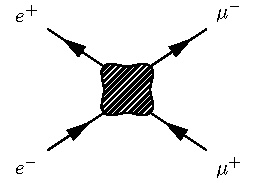
\includegraphics[width=0.25\textwidth]{feynmanDiagrams/output/ElElToMuMu}}}
            =
            \vcenter{\hbox{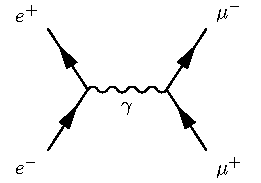
\includegraphics[width=0.20\textwidth]{feynmanDiagrams/output/ElElToMuMu_tree}}}
            +
            \vcenter{\hbox{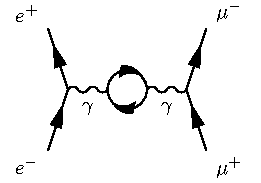
\includegraphics[width=0.20\textwidth]{feynmanDiagrams/output/ElElToMuMu_oneLoop1}}}
            \nonumber
            \\
            +
            \vcenter{\hbox{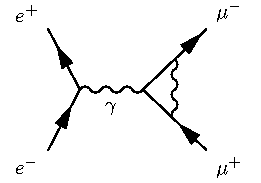
\includegraphics[width=0.20\textwidth]{feynmanDiagrams/output/ElElToMuMu_oneLoop2}}}
            +
            \vcenter{\hbox{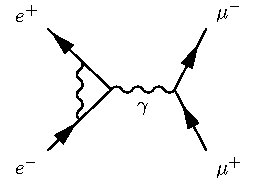
\includegraphics[width=0.20\textwidth]{feynmanDiagrams/output/ElElToMuMu_oneLoop3}}}
            +
            \vcenter{\hbox{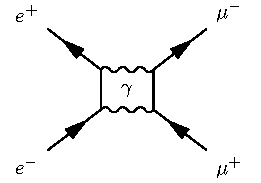
\includegraphics[width=0.20\textwidth]{feynmanDiagrams/output/ElElToMuMu_oneLoop4}}}
            +
            ...
            \nonumber
        }
        \caption{Illustration of development of the process $e^+ e^- \rightarrow \mu^+ \mu^-$
        in a model with only electrons and muons coupling to a photon. \label{fig:perturbativeDevelopment}}
    \end{figure}

    The parameters and consistency of the Standard
    Model has been extensively measured and tested in several experiments, in particular
    at the LEP experiments, the Belle and BaBar experiment, and at the Tevatron. In 2012,
    the CMS and ATLAS experiments at the LHC discovered the last remaining particle, the
    Higgs Boson with a mass $m_H \sim 125\GeV$. The full mass spectrum of the particles
    of the Standard Model is summarized on Figure \ref{fig:theory/fermionMasses} and
    shows a clear hierarchy between the different fermion generations.

    Figure \ref{fig:theory/standardModelFit} shows the result of the global fit of
    observables of the Standard Model. In such a fit, one observable at a time is set free
    while others are taken from experiment. The value of the free observable is then
    predicted from the model, and compared to its experimentally measured value. The
    difference is finally compared to the experimental uncertainty. This allows to have a
    global test of the consistency of the model, as any significant deviation between the
    predicted and measured value would indicated a flaw. The results indicate that the theory
    is consistent, as no deviation larger than 3$\sigma$ is found.

    \insertFigure{theory/fermionMasses}{0.6}
                 {Masses of the fermions and bosons of the Standard Model. The photon
                 $\gamma$, gluon $g$ and neutrinos $\nu_\ell$ are not represented as they
                 are massless in the context of the Standard Model.}

    \insertFigure{theory/standardModelFit}{0.35}
                  {Global fit of observable of the Standard Model}

    \section{Shortcomings of the Standard Model}
    %====================================================================================

    Despite its success, the Standard Model contains theoretical open questions and
    experimental facts unexplained. For these reasons, it is thought to be still incomplete
    or to be an effective theory valid only at low energy hiding a higher
    degree of symmetry at high energy. In this section, we focus especially on the hiearchy
    problem and dark matter as they will be the most relevant one in the context of this
    document, and discuss briefly other open questions.

        \subsection{The hierachy problem}

    The hierarchy problem is related to the prediction of the physical Higgs boson mass.
    Before stepping into this problem, let's first look at the case of the mass of fermions
    and gauge bosons.

    To compute a physical, observable parameter in a quantum field theory, one needs to
    integrate over all possible quantum corrections related to this parameter. In the case
    of the cross-section of a process, this means considering all loops and diagrams
    with the same initial and final state. In the case of the mass of a particle, one is
    interested to diagrams that contribute to the propagator. An example of diagram contributing
    to the propagator of the electron is given in Figure \ref{fig:feynmanDiagrams/output/electronPropagator}. We may
    express the observable mass $m_e$ of the electron as the sum of the bare mass $m^0_{e}$,
    that is to say the actual parameter inside the lagrangian, and $\Delta m_e$ representing
    the contributions from the quantum corrections :

    \eq{electronMassCorrection}
    {
        m^2_e \, = \, {m_e^0}^2 + \Delta m_e^2
    }

    \insertFigure{feynmanDiagrams/output/electronPropagator}{0.4}
                 {Example of contribution to the electron propagator.}

    For effective theories, the computation of quantum corrections is done with respect to
    an energy cutoff $\Lambda$, representing the scale at which new physics is expected
    to play a significant role. In the case of Figure \ref{fig:feynmanDiagrams/output/electronPropagator}, this mean
    that we shall integrate over all momentum inside the loop up to the scale $\Lambda$.
    For instance, if one considers electrodynamics as an effective theory of electroweak,
    at one-loop level :

    \eq{electronMassCorrection2}
    {
        \Delta m_e \, \simeq \, \frac{\alpha}{4\pi} \, m_e^0 \, \text{ln}\left(\frac{\Lambda}{m_e^0}\right)
    }

    With $\Lambda = \Lambda_{\text{electroweak}} = \orderOf{100\GeV}$, we find that
    $\frac{\Delta m_e}{m_e} \sim 20\%$. It is a relatively small correction, in the sense
    that it is not surprising to have a mass for the electron that is $\orderOf{1\GeV} \ll \Lambda_{\text{electroweak}}$.
    The most important feature in \ref{eq:electronMassCorrection2} is the fact that $\Delta m_e$
    is proportional to $m_e^0$ and not $\Lambda$ as it means the mass will not diverge
    when the scale grows.

    There is a remarkable and more general property behind this term which is that a
    gauge invariant lagrangian cannot generate corrections that are breaking the symmetry. In
    the case of electrodynamics with a massive electron, the mass term is already breaking
    the chiral symmetry $U(1)_L \times U(1)_R$, but because this is a so-called soft-breaking
    term, the property should still hold in the limit where $m_e^0 \rightarrow 0$.
    Therefore the correction cannot be proportionnal to $\Lambda$ but only to $m_e$, by
    dimensional analysis. It is common to refer to this by saying that chiral symmetry
    protects the mass of fermions from diverging. The same fact is observed for gauge
    bosons masses in the case of the electroweak symmetry breaking by the Higgs field :
    here, the gauge bosons are protected by the gauge invariance preventing the mass terms.

    Looking at the mass of the Higgs boson, it is found that the Standard Model does not include
    any mechanism that prevent the mass of a scalar boson from diverging. The actual
    computation for the correction from a fermion loop gives :

    \eq{higgsMassCorrectionFromFermion}
    {
        \Delta m_h^2 \, \propto \, m_f^2 \Lambda^2,
    }

    which diverge with $\Lambda$. If one is confident that the Standard Model is valid
    up to the Planck scale, where gravity will obviously play a significant role, then
    the observable Higgs mass is

    \eq{higgsMassCorrectionTotal}
    {
        m_h^2 \, \simeq \, {m_h^0}^2 + \kappa \cdot m^2_\text{Planck}
    }

    where $\kappa$ is a function of the Standard Model coupling and masses. The
    three quantities $m_h^0$, $\kappa$, and $m_\text{Planck}$ are \emph{a priori} unrelated
    to each other from the point of view of the theory. Unless the parameters of the
    Standard Model conspire with each other and are \emph{fine-tuned} at twenty decimal
    places, there is no reason to expect that $m_h \ll m_\text{Planck}$. However we know
    that $m_h \sim \orderOf{10^2\GeV} \ll m_\text{Planck} \sim \orderOf{10^{19}\GeV}$ which
    is not natural. This is referred to as the hierarchy problem, as from this considerations
    there is no reason to expect such a large hierarchy between the electroweak scale and
    the Planck scale.

        \subsection{Dark matter}

    Dark matter is another puzzle of current cosmology and fundamental physics in general.
    The first main observation leading to the dark matter hypothesis came from the measurement
    of rotation curves of galaxies. These curves showed the evolution of the radial velocity
    of stars inside the galaxy as function of their distance to the galactic center. One
    can predict such curves by infering the galaxy's mass repartition from models and
    spectrometry, and applying Newton's law of gravitation. The observed curves are
    well-described for the central region of the galaxy but then instead of decreasing
    with distance, stayed approximately constant.

    This observation suggested that there is a halo of invisible matter around
    galaxies, interacting gravitationnaly but not electromagnetically with the rest of the
    matter, hence the denomination \emph{dark} matter. Further experimental measurements
    provided indirect evidences for the existence of such dark matter. One of the main
    ones are using the technique of gravitational lensing that allows the observer to
    infer the mass of a galaxy or a cluster from the bending of the light emitted by
    an object further in the background. Nowadays, dark matter is part of the standard
    model of cosmology as there are many astrophysical and cosmological phenomenom which
    cannot be described without it, and has been found to represent $\orderOf{80\%}$ of
    the matter content of the universe.

    However the nature of dark matter is still unknown and no clear direct evidence has
    been found for it. It is now commonly admitted that there is no suitable candidate
    for it in the Standard Model. Dark matter candidates must be gravitationally interacting,
    not be short-lived and must not be baryonic. Last but not least, it must also be
    cold, that is to say that it must have low kinetic energy.

    If one assume that dark matter is made of a single particle $X$, a simple model gives that
    the relic density $\Omega_X$ is proportionnal to $m_X^2 / g^4_X$ where $m_X$ is the
    mass of the dark matter particle and $g_X$ is the coupling constant in the process
    $XX \leftrightarrow q\bar{q}$. It is remarkable to note that taking $\Omega_X = \orderOf{0.1}$
    from cosmological observations and $g_X \sim 0.6$ from the weak interaction, then
    we expect $m_X = \orderOf{100\GeV}$. This encourage physicist to look for weakly
    interacting massive particles (or WIMPs) which are predicted by many models beyond
    the Standard Model.

        \subsection{Other open questions and criticism}

    Other open questions or unexplained facts add fuel to the belief that the Standard Model
    is not the final theory.

    \begin{itemize}
        \item \textbf{Dark energy} - The standard model of cosmology, so-called $\Lambda$CDM model,
            contains a non-null cosmological constant called $\Lambda$. The cosmological
            constant is initially an additional authorized term in Einstein's equation
            which relates space-time curvature to energy-momentum. Such term is necessary
            to explain the observed accelerated expansion of the universe from the study
            of the redshift of supernovas. The cosmological constant can be interpreted
            as vacuum energy, often referred to as dark energy. Despite the fact that this
            is in principle in agreement with quantum field theory which predicts vacuum
            energy from vacuum quantum fluctuations, there is a complete mismatch, of $\orderOf{10^{120}}$,
            between the small measured value of $\Lambda$ and its prediction
            by quantum field theory. This is often called the vacuum catastrophe or the worst
            prediction in the history of physics. A big challenge of current physics therefore
            consists in understanding the nature of dark energy and why it is so small
            compared to prediction.
        \item \textbf{Matter-antimatter asymmetry} - It is a well established fact that
            the baryonic content of the Universe is made of matter. Because matter and antimatter
            should have been produced in equal proportion during the big bang, there must
            be sources of asymmetry that led to a state dominated by matter. Sakharoved
            established a set of conditions that would
            induce such an asymmetry. Among them is that the symmetries C and CP, i.e. inversion
            of charge and inversion of both charge and parity, is violated. The Standard Model
            with massless neutrinos contains two sources of CP-violation originating from
            the CKM matrix and the CP-violating phase in the QCD sector. So far however,
            these sources are not important enough to explain the magnitude of the baryon
            asymmetry.
        \item \textbf{Neutrino masses} - It has been measured by experiments that neutrinos
            can oscillate from one flavor to another. This indicate that neutrinos should
            be massive and have different flavor states than mass states much like down-type
            quarks and the CKM matrix. The problem of neutrino being massive is itself not
            so much a problem as it is possible to introduce right-handed neutrinos in the
            field content of the Standard Model. However the exact mechanism depends of
            wether neutrinos are Dirac or Majorana fermions. The main source of interrogation
            is to understand why neutrinos have such a small mass compared to the other
            fermions.
    \end{itemize}

    \begin{itemize}
        \item \textbf{Strong CP problem} - As introduced before, there is a term allowed in
            the QCD lagrangian that introduces CP-violation via a phase $\theta$. The value
            of this parameter has been so far found to be very close to zero despite
            lack of theoretical arguments for it not to be of the order of 1. This is a situation
            similar to the hierarchy problem where we can expect that there is a mechanism
            at stake protecting this phase to be too different from zero.
        \item \textbf{Quantum gravity description} - Gravitation is currently not described
            by the Standard Model. This underlying problem, which is to know how to unify general
            relativity with quantum field theory, is one of the biggest problem of modern
            physics. If it exists, the gauge boson associated to the gravitation would
            need to have a spin equal to 2. It is however not known if and how such
            a theory would be renormalizable as it leads to uncancellable divergences.
        \item \textbf{Forces unification} - Several times in the history of physics,
            phenomenons have been understood to have a common structure and
            been unified. The simple name electromagnetism has in its ethymology a clear
            reference to electrodynamic and magnetism. It is therefore natural for physicist
            to look for possibilities of unification, in our case regarding the electroweak
            and strong interaction, and ultimately with gravitation. \todo{mention coupling constant convergence}

        \item \textbf{Free parameters and arbitrary field content} -
            Finally, there are conceptual interrogations about the fact that the quarks have
            such different masses, in particular regarding the top quark as it is the
            heaviest known particle. The same kind of conceptual interrogations goes about
            the number of fermion families : is there any fundamental reason to have three
            families instead of one, two, or an infinity of them ? More generally, there
            are numerous fact about the Standard Model parameters and field content that
            feel arbitrary and may hide an underlying, more fundamental pattern.
    \end{itemize}


    \section{Theories beyond the Standard Model}
    %====================================================================================

        \subsection{Zoology of Standard Model extensions}

        Since a few decades, extensions to the Standard Model have been proposed and
        studied with the aim to adress its shortcomings. One can attempt to categorize
        them as function of the fundamental ingredient they add to the theory, either
        additional symmetries, space-time dimensions or field content.

            \subsubsection{Additional or extended symmetries}
            % -> particles / gauge / space-time

        One of the possibility to extend the Standard Model is to look at symmetries.
        There are however different kind of symmetries, which do not impact the theory
        the same way, namely space-time symmetries or gauge symmetries. The only possible
        extension of space-time symmetries is supersymmetry which is discussed later
        in a dedicated section.

        It's possible to think about gauge groups which include the Standard Model group,
        $SU(3) \times SU(2) \times U(1)$ to create Grand Unification Theories (GUT) in which
        the coupling constants are unified. Such groups are also motivated because they
        naturally introduce a symmetry between leptons and quarks as one can think of
        when looking at the pattern of the Standard Model.

        The most simple group one can find is $SU(5)$ which would be a broken symmetry at
        low energy just as the electroweak symmetry is. Rotations in the $SU(5)$ space
        can mix the quark and lepton fields which led to a prediction of proton decay
        incompatible with experimental measurements. Grand-unificiation with $SU(5)$ is
        now mostly abandonned but remains an idea studied for larger groups such as $SO(10)$.

            \subsubsection{Additional dimensions}

        The second possibility is to add extra space-time dimensions. While everyday's life
        is only composed of 3+1 (space and time) dimensions, theoretical mechanism have been
        discovered that could explain why additional dimensions are noticeable at our scale.
        The extra dimension is usually considered to be a space-like dimension, as an
        additional time-like dimension would break causality. Extra dimensions theories
        are of particular interest for unifying interaction with gravitation and answering
        the hierarchy problem.

        Large extra dimensions (ADD) theories are based on the idea that the Standard Model
        interactions take place only in the four dimensions and gravity would be
        allowed to travel in the extra dimensions. At large distances, gravity would
        be diluted while at low distances (i.e. high energies) the Standard Model interaction
        and gravitation would have coupling constant that are of the same order. A phenomenological
        consequence is that microscopic black holes could be produced in high-energy collisions
        provided that the collision probe distances lower than the Schwarzschild radius.

        The Randall-Sundrum (RS) scenarios consider a five dimensions universe made of two
        four dimensions branes separated by an extremely warped fifth dimension. One of
        the brane corresponds to the Standard Model physics while the other brane would be
        the realm of gravity. The distance separating the two brane is directly linked to
        the difference of energy scale between the Standard Model sector and the gravitation
        sector. A phenomelogicial prediction of these models is the production of gravitaton
        excitations at the TeV scale.

        Finally, universal extra dimensions (UED) theories are based on the idea that
        the extra dimensions are compactified such that they are not noticeable at macroscopic
        scales. An useful analogy to understand the compactification of a dimension is
        consider that, for instance, a guitar string seen from very far looks like a one-dimensional
        object whereas if seen from very close exhibits a second periodic dimension around
        the string axis because of its thickness. The additional dimensions are therefore
        parametrized as function of a radius. Phenomenologically, one would observe a discrete
        mass spectra for the Standard Model particles corresponding to excitations along
        the compactified dimensions.

            \subsubsection{Additional or modified field content}

        A third possibility is to introduce new ad-hoc fields of modify existing ones
        to adress the shortcomings of the Standard Model.

        One first elegant idea following this principle is to explain the lightness of the
        Higgs by considering it is a composite object. This idea is inspired from QCD where
        light scalars are encountered and do not exhibit a naturalness problem. Pions,
        for example, can be seen as Goldstone bosons of the spontanneous breaking of chiral
        symmetry, and therefore are massless. However in practice, chiral symmetry is not exact as
        the underlying quarks do have mass, thus pions are only pseudo-Goldstone boson and get a mass,
        but they are still protected by the approximate chiral symmetry from being heavy.
        Applying the same idea to the Higgs would therefore answer the hiearchy problem.
        This also means that there would be a new interaction whom the Higgs would
        be just the lightest hadron-like state and other state could be seen at higher
        energy. Another indication of compositeness would also come from different couplings
        to gauge bosons.

        Other hypothesis of new fields include axions, an idea first introduced to solve
        the strong CP problem and eventually led to a dark matter candidate. Axions would
        have masses lower than $\orderOf{1~\text{eV}}$ while still satisfying criteria to
        be cold dark matter candidates.

        Focusing on the search for dark matter candidates leads to proposing that dark matter
        is not made of just one, but several kind of particles regrouped in the concept
        of an hidden sector. There are several possibilities to describe the link between
        the Standard Model and this hidden sector, for instance by assuming that the Higgs
        relate the two sectors, or by ntroducing a new
        $U(1)_H$ gauge group whose gauge boson would be a so-called dark photon.

            \subsubsection{The anthropic principle}

        Finally, one of the alternative to theories beyond the Standard Model is to
        simply accept the Standard Model as it is. This is strongly related to Einstein's
        interrogation regarding if Nature had any choice at teh creation of the universe.
        It can be argued that most of the shortcomings of the Standard Model related to
        gravitation and cosmology might simply be unsolvable at scales accessible by
        particle physics experiments. The most important remaining issue are related to the
        fine-tunning in the hierarchy problem and the arbitrary of the other parameters of
        the theory.

        The anthropic principle states that when studying the universe, it
        should be taken into account that conscious life is possible in it. It might be
        that our universe is simply one realization of universe among many others in what
        is called a multiverse. What appears as to be fine-tunning would in fact be
        equivalent to natural selection at the scale of the mutiverse where the observed
        universes can only be the one allowing conscious life.

        This view is however controversial as it yields very little if no testable
        prediction except understanding how likely life would be if the parameters of
        the Universe would have been different \todo{0807.3697v1}.

        \subsection{Supersymmetry}

        \subsubsection{General idea and motivations}

        Here, we propose to have a dedicated look at the idea of Supersymmetry. Supersymmetry,
        abbreviated SUSY, emerged around the 70's and designates a symmetry between bosons
        and fermions. Mathematically, we can write such a transformation :
        \eqalign{SUSYtransformation}
        {
            Q \rvert \text{F} \rangle \rightarrow \rvert \text{B} \rangle \nonumber
            \\
            Q \rvert \text{B} \rangle \rightarrow \rvert \text{F} \rangle
        }
        where the subscript $f$ and $b$ refer to fermion and boson. Here, $Q$ is a \emph{global}
        symmetry, i.e. it does not depend of space-time, and is therefore not a gauge
        symmetry. As it relates two states with different spins, it must itself have a
        spin 1/2. This means \todo{but why...} that SUSY is a space-time symmetry
        in the sense that it is a non-trivial extension of the Poincaré algebra. This is
        an important consideration : it has been demonstrated by Colemand and Mandula \todo{ref} that
        the only possible symmetry of Nature are the Poincaré symmetry and the gauge
        symmetries. Haag, Lopuszanski and Sohnius later relaxed this theorem by
        noticing that another type of symmetry is possible and precisely corresponds to
        supersymmetry. \todo{Haag, Lopuszanski, Sohnius, 1975}

        A remarkable property of SUSY is that trying to gauge it, meaning making the
        transformation space-time dependent, yields a description of gravitation called
        supergravity or, abbreviated, SUGRA. Supersymmetry also provides a link with
        string theory which is a candidate of theory of everything.

        To each fermion is therefore associated a boson with same charges, to each boson
        is associated a fermion. The particule associated to another by SUSY is called
        superpartner, and can be put together in a superfield. To ensure the consistency
        of the theory\todo{check this}, superpartners of vector bosons have spin 1/2 and superpartners
        of fermions have spin 0.  SUSY alone predicts that a particle and its superpartner
        should have the same mass. However this cannot be the case in pratice as no
        such thing has been observed by experiments, meaning that supersymmetry must be
        a broken symmetry.

        There are several mechanism that are candidate to spontanneously break SUSY. Some
        are based on a gravity mediated supersymmetry breaking, others involve a gauge
        mediated mechanism, and another possibility is to have an anomaly mediated breaking.
        Since the exact mechanism is unknown at the moment, one solution is to simply add
        a $\mathcal{L}_\text{soft}$ component to the lagrangian that includes all allowed
        terms and corresponding new parameters.

        One of the main motivation for supersymmetry is to provide a mechanism that
        protects the mass of scalar bosons, thus answering the hierarchy problem. In the
        case of the Higgs boson, one can show
        that if the superpartners have equal masses, then the quadratic divergences
        introduced in \ref{eq:higgsMassCorrectionFromFermion} cancel each other and
        it gets natural for the Higgs to have a mass much lower than the Planck scale.
        If SUSY is only softly broken, as for chiral and gauge symmetry, then the
        boson-fermion symmetry still prevents to have a quadratic divergence. Instead,
        we are left with a mild logarithmic divergence :
        \eq{higgsMassCorrectionInSUSY}
        {
            \Delta m_h^2 \, \propto \, (m_f^2 - m_b^2) \, \text{ln}\left(\frac{\Lambda}{m_b}\right).
        }
        But this alone does not solves everything. If one consider the most massive
        fermion, that is the top quark $t$, then the mass ratio with its superpartner the
        stop $\tilde{t}$, $r = m_{\tilde{t}} / m_t$ cannot be too large. For instance, if
        $r = 100$ then we are left with corrections $\Delta m_h = \orderOf{100 \cdot m_t}$
        which is still large considering that we seek $\orderOf{m_h} = \orderOf{m_t}$.
        Therefore, we would need to reintroduce a certain level of fine-tunning to the
        parameter of the model for the corrections to cancel, and we want to avoid that
        to keep the theory natural. Hence, the naturalness of SUSY is strongly related to
        the mass of the superpartners of heavy fermions such as the top and bottom quarks.

        \subsubsection{The MSSM}

        The most studied realization of supersymmetry is the minimal supersymmetric standard
        model, or MSSM, corresponding to adding the minimum number of fields to the Standard
        Model for it to become supersymmetric. \todo{ref to The Minimal Supersymmetric
        Standard Model / Jorge C. Romao, and  hep-ph/9612229 SUSY and Such / Dawson}
        Since the MSSM breaks SUSY with ad-hoc terms, it is to be seen as an effective
        theory up to $\Lambda_{\text{SUSY breaking}}$.

        At each fermion and gauge boson is therefore associated a superpartner that we may
        call sfermion and gaugino. It should be
        stressed once again that left-handed and right-handed fermions are different
        fermions. Hence, there are for example two selectrons, one associated to
        each chirality of the electron. These are usually noted $\tilde{e}_R$ and $\tilde{e}_L$
        to associate them easily with their fermion partner, even though they are spinless.
        Regarding the Higgs sector, it is necessary to add not only a superpartner called
        higgsinos, but a second Higgs field to ensure the concistency of the theory.

        As shown in the case of the Standard Model, the mass eigenstates are not
        necessarily the flavor eigenstates. This is still true in the MSSM, especially
        because of the SUSY breaking terms, and is an important consideration for the
        phenomenology. In particular, masses eigenstates are formed by the combinations of
        the Higgsinos and electroweak gauginos and are called charginos and neutralinos.
        For the fermions, mixing terms are authorized in $\mathcal{L}_soft$ between the
        left and right-handed superpartners and are especially important for the
        phenomenology of the third generation. The masses eigenstates can be determined
        by diagonalizing the mass matrices. The resulting particles spectrum is given on
        Table \ref{tab:MSSMsuperpartners}.

        \begin{table}
            \centering
            \begin{tabular}{ccc}
                \textbf{Flavor eigenstates} & & \textbf{Mass eigenstates} \\
                                            & & \\
            \begin{tabular}{|ccc|}
                \hline
                1$^\text{st}$ gen. & 2$^\text{nd}$ gen. & 3$^\text{rd}$ gen. \\
                \hline
                \hline
                $\tilde{u}_L$        &   $\tilde{s}_L$      & $\tilde{t}_L$ \\
                $\tilde{u}_R$        &   $\tilde{s}_R$      & $\tilde{t}_R$ \\
                $\tilde{d}_L$        &   $\tilde{c}_L$      & $\tilde{b}_L$ \\
                $\tilde{d}_R$        &   $\tilde{c}_R$      & $\tilde{b}_R$ \\
                \hline
                \hline
                $\tilde{\nu}_e$      &   $\tilde{\nu}_\mu$  & $\tilde{\nu}_\tau$ \\
                $\tilde{e}_L$        &   $\tilde{\mu}_L$    & $\tilde{\tau}_L$   \\
                $\tilde{e}_R$        &   $\tilde{\mu}_R$    & $\tilde{\tau}_R$   \\
                \hline
            \end{tabular}
            &
            &
             \begin{tabular}{|ccc|}
                \hline
                1$^\text{st}$ gen. & 2$^\text{nd}$ gen. & 3$^\text{rd}$ gen. \\
                \hline
                \hline
                "       &  " & $\tilde{t}_1$ \\
                "       &  " & $\tilde{t}_2$ \\
                "       &  " & $\tilde{b}_1$ \\
                "       &  " & $\tilde{b}_2$ \\
                \hline
                \hline
                "       &  " & "                  \\
                "       &  " & $\tilde{\tau}_1$   \\
                "       &  " & $\tilde{\tau}_2$   \\
                \hline
            \end{tabular}
            \\
            & $\rightarrow$ & \\
            \begin{tabular}{|ccc|}
                \hline
                Higgs   & Electroweak         & Strong          \\
                sector  & sector              & sector          \\
                \hline
                \hline
                $\begin{matrix} \tilde{h}^0_u, \tilde{h}^+_u \\ \tilde{h}^0_d, \tilde{h}^-_d \end{matrix}$
                &
                $\begin{matrix} \tilde{B} \\ \tilde{W}_{1,2,3}\end{matrix}$
                &
                $\begin{matrix} \tilde{g}_{1..8} \end{matrix}$ \\
                \hline
            \end{tabular}
            & &
            \begin{tabular}{|cc|}
                \hline
                Charginos and   & Strong          \\
                neutralinos     & sector          \\
                \hline
                \hline
                $\begin{matrix} \tilde{\chi}^\pm_{1,2} \\ \tilde{\chi}^0_{1,2,3,4} \end{matrix}$
                &
                "
                \\
                \hline
            \end{tabular}
            \end{tabular}
            \caption{Superpartners of the fermions and bosons of the standard model,
            categorized according to flavor eigenstates (on the left) and masses eigenstates
            (on the right). A symbol " indicates that the mass eigenstate is identical to
            flavor eigenstate. \label{tab:MSSMsuperpartners}}
        \end{table}

        By design, the MSSM conservs a quantum number called R-parity defined as \todo{define J and B}:
        \eq{RparityDefinition}
        {
            R = (-1)^{2J + 3B + L}.
        }
        $R$ is 1 for the particles of the standard model and -1 for their superpartners.
        As it is conserved, this means that supersymmetric particles can only be
        pair-produced and only decay to an odd number of supersummetric particles. In
        particular, this means that the lightest supersymmetric particle is stable as
        its decay would violate the $R$-parity. The important consequence is that it provides
        a good candidate for dark matter, provided that this particle is neutral.

        \subsubsection{Phenomenology of the chargino, neutralino and stop sector}

        \todo{explicit link between the parameters and mixing matrix + detail on
        coupling stop-top-EW}

        In the $(\tilde{B}, \tilde{W}^3, \tilde{h}^0_1, \tilde{h}^0_2)$ basis,
        \eq{charginoMixingMatrix}
        {
            M_{\tilde{\chi}^0}
            =
            \begin{pmatrix}
                \tilde{m}_{\tilde{B}} & 0                     & - m_Z \,\text{cos}\, \beta \,\text{sin}\, \theta_W &   m_Z \,\text{sin}\, \beta \,\text{sin}\, \theta_W
                \\
                0                     & \tilde{m}_{\tilde{W}} &   m_Z \,\text{cos}\, \beta \,\text{cos}\, \theta_W & - m_Z \,\text{sin}\, \beta \,\text{cos}\, \theta_W
                \\
                - m_Z \,\text{cos}\, \beta \,\text{sin}\, \theta_W  &   m_Z \,\text{cos}\, \beta \,\text{sin}\, \theta_W & 0 & \mu
                \\
                  m_Z \,\text{sin}\, \beta \,\text{sin}\, \theta_W  & - m_Z \,\text{sin}\, \beta \,\text{cos}\, \theta_W & \mu & 0
            \end{pmatrix}
        }

        In the $(\tilde{W}^\pm, \tilde{h}^\pm)$ basis
        \eq{charginoMixingMatrix}
        {
            M_{\tilde{\chi}^\pm}
            =
            \begin{pmatrix}
                \tilde{m}_{\tilde{W}}
                &
                \sqrt{2} m_W \,\text{cos}\, \beta
                \\
                \sqrt{2} m_W \,\text{sin}\, \beta
                &
                \mu
            \end{pmatrix}
        }

        In the $(\tilde{t}_L, \tilde{t}_R)$ basis,
        \eq{stopMixingMatrix}
        {
            M_{\tilde{t}}
            =
            \begin{pmatrix}
                \tilde{m}^2_{\tilde{t}_L} + m^2_t + m^2_Z(\frac{1}{2} - \frac{2}{3} \,\text{sin}^2 \theta_W) \,\text{cos}\, 2\beta
                &
                m_t ( X_{\tilde{t}} + \mu \,\text{cot}\, \beta)
                \\
                m_t ( X_{\tilde{t}} + \mu \,\text{cot}\, \beta)
                &
                \tilde{m}^2_{\tilde{t}_R} + m^2_t + \frac{2}{3} m^2_Z \,\text{sin}^2 \theta_W \,\text{cos}\, 2 \beta
            \end{pmatrix}
        }
        with :
        \begin{itemize}
            \item $\tilde{m}_p$ the mass terms for $p$ coming from the soft-breaking SUSY terms
            \item $m_p$ the mass term for $p$ coming from the electroweak symmetry breaking
            \item $X_{\tilde{t}}$ characterizing the trilinear coupling between the top partners and the Higgs field
            \item $\text{cos}\,\theta_W \definedAs m_W / m_Z$ defines the weak mixing angle
            \item $\mu$ and $\text{tan}\, \beta \definedAs v_2 / v_1$ relates the Higgs sector
        \end{itemize}




%==============================================================
\setcounter{mtc}{2}
\chapter{The Compact Muon Solenoid experiment at the LHC}
\minitoc
\newpage
%==============================================================

    \section{The Large Hadron Collider}

    \todo{references !!}

    \todo{clarify incident / run I at 7/8 TeV, run II will be at 13 TeV}

    \todo{mention that the Higgs has been discovered}

    \subsection{Scientific context and challenges}

    There are several approaches one can take toward new physics. First, using already
    available measurement of observables and exploiting the fact described in \ref{standardModelSuccess}
    that observables are impacted through loops by the entire Nature's lagrangian,
    it's possible to infer information or limits regarding yet-unknown physics. Historically,
    this has been proved successful numerous times, for instance to predict the
    mass of the top quark from the $W$ boson mass. Similarly, a smoking-gun for some
    supersymmetric model is the enhancement of the branching ratio BR($B_s \rightarrow \mu^+\mu^-$).
    However, despite the fact this approach provides valuable information, it can
    be criticized as only providing indirect evidences and not a clear window to new phenomena.
    Moreover, the statistics and detector resolution required to increase the accuracy
    of the prediction grows exponentially.

    The most attractive and fruitful approach is of course the direct observation of
    new phenomena. One often forgotten fact is that new physics might not appear at high
    energies but at low energies instead. This is motivated for intance by by axions
    theories and some hidden sector theories which predict particles with sub-eV masses
    or rare interactions. Nevertheless it is more common to assume that new physics will
    show up at high energies. To probe higher energies, particle colliders have been
    built with increasing center of mass energies ($\sqrt{s}$) during the last centuries.
    Two famous ones are the Large Electron-Positron (LEP) collider and the Tevatron. The
    LEP was an $e^+e^-$ collider which operated at a maximum of $\sqrt{s} \approx 200\GeV$
    at CERN in the 90's and led to the discovery and study of the $Z$ and $W$ bosons. The
    Tevatron was a $p\bar{p}$ collider which operated at a maximum $\sqrt{s} \approx 2\TeV$
    at Fermilab until 2011. Nowadays, the only high energy collider in operation is the
    Large Hadron Collider (LHC) at CERN.

    The LHC is a circular hadron collider built at CERN, near Geneva. One of its physics
    goal is the production high-energy proton-proton ($pp$) collisions to explore physics around
    $1\sim10 \TeV$ to test the validity of the Standard Model and possibly discover new
    physics. It is also capable of producing heavy ions (PbPb) collisions or proton-ion
    collision ($p$Pb) to study nuclear physics at high energy, in particular the properties
    of quark-gluon plasma. The rest of this
    document will focus on $pp$ collisions.

    The LHC collider has been built using the same tunnel as the LEP. The beam energy at
    the LEP was largely limited by the energy loss from synchrotron radiation. This loss
    is proportional to $E^4 / (m^{4} r^{2})$ with $E$ and $m$ the energy and mass of the
    particle, and $r$ the radius of the tunnel. As $m_p$ is much larger than $m_e$, it is
    easier to maintain the energy of a rotating proton beam than an electron/positron one.
    Consequently, using protons is preferred if the goal is to reach the highest possible
    energy, justifying this choice for the LHC. We will see in section
    \ref{sec:physicsFromCollisionsAtTheLHC}, how proton collisions are however challenging
    from a reconstruction and analysis point of view.

    \subsection{Beam injection, control and acceleration}


    The creation and first acceleration of the proton beam work as follow. Protons are initially
    produced by heating low-pressure $H_2$ gas which produces $H^+ = p$ and $e^-$ and
    separating the protons using high voltages. The protons are fed to an acceleration
    chain made of consecutive accelerators which use radiofrequencies to create an acceleration
    gradient. At the end of the chain, in the Super Proton Synchrotron (SPS), the
    beam acquired an energy of $450\GeV$ before being injected in the LHC ring. The LHC
    ring is a tunnel of 27 kilometers built between $50$ and $200$ m underground. The
    project was originally designed to accelerate the proton beam up to $7\TeV$ per beam,
    corresponding to a center of mass energy $\sqrt{s} = 14\TeV$. Four experiments are
    installed along the ring, at each collision point. Two of them, ATLAS and CMS, are
    general-purpose experiments while ALICE focuses on heavy-ion collisions and LHCb studies
    $b$-hadrons properties. Figure \ref{fig:LHClayout} presents an overview and the general
    layout of the machine.

    \insertTwoFigures{LHClayout}
                     {LHC/LHCring}
                     {LHC/LHClayout}
                     {0.6}
                     {On the top, sketch of the underground installation showing the SPS
                     and the injection tunnels as well as the four experiments. On the bottom,
                     layout of the LHC ring. The installation is divided in eight octants,
                     with some of them dedicated to collisions but also injection, acceleration (RF)
                     and beam dump.}

    One of the biggest challenge of the LHC was the construction and operation of magnets
    powerful enough to bend the trajectory of the protons at such high energies. To do
    so, superconducting magnets made of a niobium-titanium alloy are used and are able to
    produce a magnetic field of up to $8.33$ T. The operating temperature of such magnets
    is only a few Kelvins : in the context of the LHC, they are required to be cooled using
    a complex system of superfluid helium-4 at 1.9K. It is remarkable to note that this
    temperature is actually cooler than the cosmic microwave background at $\approx2.7$ K.

    Operating superconducting magnets require a good control and understanding of quenches.
    A magnet quench occurs when a part of the superconducting material loose its superconducting
    property and starts to heat because of Joule effect. Because the critical temperature
    is usually low, this can create a chain reaction as the heat spread. Quenches are
    not such unusual events, and the LHC employs a sophisticated system to detect them and protect
    the magnetic system by automatically dumping the beam, mitigating the effect of the
    quench and extracting the energy stored inside the magnet.
    \todo{http://cerncourier.com/cws/article/cern/54383}. However, deffects in the protection
    system or more generally in the electrical and mechanical apparatus can have dramatic
    impact as the energy can easily damage the machine if released improperly. In 2008,
    a faulty electrical interconnection between two magnets led to an electrical arc that
    punctured the cryogenic fluid enclosure and vaporized a fraction of the fluid causing
    important damages to the installation.

    %\insertFigure{LHC/pipePhoto}{0.7}{\todo{caption} Credit : Maximilien Brice, CERN}
    \insertTwoFigures{LHCpipe}
                     {LHC/dipoleCrossSection2}
                     {LHC/pipePhoto2}
                     {0.7}
                     {On the top, cross-section of a cryodipole of the LHC
                     \todo{ref to LHC Machine / JINST 3 S08001 doi:10.1088/1748-0221/3/08/S08001},
                     showing the magnet coils around the two beam pipes, and the cooling system.
                     On the bottom, technician working on an interconnection between two LHC
                     sections (credit : Anna Pantelia, CERN).}

    The pipes of the LHC consist of about 1200 dipole sections represented on Figure
    \ref{fig:LHCpipe}, each $15$ m long, whose role are to bend the beam using dipole
    magnets. About 400 quadrupole magnets that are used to squeeze the
    beam. Higher multipolar magnets are also used to prevent and correct instabilities of
    the beam. The effective bending radius, created from the $17.6$ km of dipoles is
    $r \approx 2.8$ km, to be compared to the radius of the full machine being about $4.3$km.

    The beam is organized in bunches of protons separated by a time interval of 50 or
    25 ns depending of the machine configuration. Each bunch is made of about $10^{11}$
    protons. The LHC uses radiofrequency cavities to increase the energy of the beam by
    about 0.5 MeV per rotation, or $5.4\GeV$ per second. At $7\TeV$ per beam with 25 ns
    between bunches, the total energy of the beam is about 360 MJ and the energy stored
    in the magnet system is about 600 MJ, roughly corresponding to the energy of a
    lighting bolt. The beams are then made to collide at four different points along the
    ring, corresponding to the four main experiments.

        \subsection{Physics of $pp$ collisions \label{sec:physicsFromCollisionsAtTheLHC}}

    The number of $pp$ collisions happening per unit of time is characterized by the
    instanteneous luminosity $L$ which depends of the bunch crossing frequency, the
    number of bunches and proton per bunches and other beam and geometry parameters.
    The two general purpose experiments, ATLAS and CMS, aim for a peak luminosity
    $ L = 10^{34} \text{cm}^{-2} \text{s}^{-1} = 10 \text{nb}^{-1} / \text{s}$. For a
    given process, one can compute the number of expected events.

    $$ n_\text{event} = L \times \sigma_\text{process} $$

    where $\sigma_\text{process}$ is the cross-section of the process and $n$ a number
    of event per unit of time. Later, we may refer to the integrated luminosity over all
    data-taking which relates to $N$, the total number of events produced.

    Figure \ref{fig:LHC/ppCrossSections} shows the evolution of the cross section of different
    processes such as $W$ or $Z$ production. The total inelastic cross section is about
    60 mb. At peak luminosity and with a bunch crossing every 25 ns, this corresponds
    to 15 inelastic interactions per bunch crossing on average. This is what is behind
    the notion of pile-up : one event, or collision, contains $\orderOf{10-30}$
    interactions with generally only one is of interest, such as the production of a $W$
    or $Z$ boson.

    \insertFigure{LHC/ppCrossSections}{0.5}{Evolution of the cross sections of typical
    processes for $p\bar{p}$/$pp$ collisions as function of $\sqrt{s}$. Two vertical
    lines corresponds to the center of mass energy of the Tevatron ($\sqrt{s} \approx 2\TeV$)
    and the LHC ($\sqrt{s} = 14\TeV$) \todo{ref to  arXiv:0812.2341}}

    This is a crucial point in the context of $pp$ collisions, as inelastic hadron collisions
    naturally produce jets arising from the parton showering and hadronization of gluons
    and quarks. Therefore, a lot of particles polute the environment of each event, affecting the
    number of impact in the tracking detector and energy measurement in calorimeters.
    It is thus needed to develop methods to mitigate the effect of pile-up.

    Furthermore, when considering one process of interest, it must be kept in mind that
    protons are composite objects made of partons, i.e. quarks and gluons, among which three
    valence quarks. At a given moment, a parton only carries a fraction of the total
    proton momentum. This is described by the parton distribution functions (PDF), characterizing
    the probably to find a parton with a fraction of impulsion $x$, depending of its
    nature. This implies that the center of mass energy of the two incoming partons is in
    fact always lower than the beam energy. Each incoming parton may also radiate partons
    right before the interaction, a processus called initial state radiation, leading to
    additional jets in the event. Finally, the remaining partons may interact with each
    other in what is called the underlying event, and produce high-energy jets, almost
    collinear to the beam axis.  $pp$ collisions
    are therefore complex processes, as summarized in Figure \ref{fig:LHC/ppCollision}, due
    to the composite nature of the proton and the fact that the parton are colored objects.

    \todo{PDF plot}

    \insertFigure{LHC/ppCollision}{0.65}{Feynman diagram showing the complexity of a
    single proton-proton collision. Two partons from the incoming protons partipate
    to the hard scattering leading to a $\gamma^*/Z$ resonnance which decays into two
    quarks. In both the initial and final states, the coloured particles may radiate gluons
    (or a gluon may split into a quark pair), leading to initial and final state radiations.}

    % Estimate of price/event ?

    \section{The Compact Muon Solenoid experiment}

        The CMS experiment is one of the four experiments installed at the collision
        points of the LHC. It is a general purpose experiment, though mostly dedicated
        to the study of $pp$ collisions, in particular to test the validity of the Standard
        Model, to understand the electroweak symmetry breaking, and to search for new physics. From this
        perspective, CMS is in scientific cooperation and competition with ATLAS, the
        other general purpose experiment. In the context of the search for new physics,
        having two experiments independently studying the same phenomenons is both
        stimulating but also crucial to have robust claims. It can indeed be
        argued that having two experiments both seeing a $3\sigma$ discrepancy is more
        convincing than one experiment seeing a $5\sigma$ discrepancy with no possibility
        of cross-checkign the result.

        In this section, the CMS detector will first be introduced generally before inspecting
        each subsystems. Then, the trigger system that aim to select which collisions to
        record will be presented. Finally, it will be explained how the physics objects
        can be reconstructed from the information recorded by the detector.

        \subsection{The CMS detector}

            \subsubsection{Physics motivations and detector overview}

        The CMS detector is an instrument that answer the fantastic challenges posed by
        the LHC machine while providing good measurement for physics purpose.

        The subsystems of the detector must indeed have a time response lower than 25 ns,
        corresponding to the design bunch crossing frequency, and to be synchronized with
        each other. The detector must also be able to disentangle between the
        $\orderOf{10-30}$ collisions occuring at each bunch-crossing by being able to
        reconstruct the collision vertices with good precision. Last but not least,
        the quantity of data per event is such that all events cannot be recorded. The
        detector must then decide in real time which events to keep, and which to reject
        from a fast analysis of each events.

        Among the many physics signature CMS aims to look at, the discovery and study of a
        light ($\orderOf{125 \GeV}$) Higgs boson in the channels $h\rightarrow\gamma\gamma$
        and $h\rightarrow ZZ \rightarrow 4\ell$ requires good measurements of the photon,
        electron and muon energy-momentum. Furthemore, from the perspective of final
        states involving dark matter candidates, one needs to obtain a good measurement
        of the energy escaping detection. This requires a good and an as hermetic as
        possible measurement of the repartition of the hadronic and electromagnetic energy
        in each event.

        The CMS detector is a heremetic, cylinder-shaped detector consisting of several
        layers dedicated to a given task as represented on Figure \ref{fig:CMS/detectorOverview}.
        Near the interaction point in the beam pipe is found the system is dedicated to the
        detection of impacts left by charged particles. It is composed of a pixel detector
        layers and microstrip layers. Around the tracking system is the electromagnetic
        calorimeter, whose aim is to measure the energy of photons and electrons using
        scintillation crystals. The next layer, the hadronic calorimeter, aims to measure
        the energy carried by hadrons produced in the collisions. It is a scintillator made
        of brass and plastic sandwich. The superconducting magnet provides a strong magnetic
        field of 3.8 T using the same technology than the LHC magnets, a nobium-titanium
        alloy, to bend the trajectory of charged particles. Finally, the muon system uses
        three different technologies to record the impact of muons.

        \insertFigure{CMS/detectorOverview}{0.9}{Overview of the CMS detector.}

        The coordinate system $(x,y,z)$ of CMS, represented on Figure \ref{fig:CMS/coordinateSystem},
        is defined such that $x$ is directed to the center of the LHC, $y$ points toward
        the sky and $z$ is colinear to the beam axis. As the detector exhibits a
        cylindrical symmetry, it is convenient to work with the azimuthal angle $\phi$
        between the momentum $\vec{p}$ of a particle and the $x$ axis in the transverse
        plane. The projection of $\vec{p}$ in the transverse plane is called $\vec{p}_T$.
        Additionnaly, the pseudo-rapidinity $\eta$ is defined by :

        $$ \eta \definedAs - \text{ln}(\text{tan}\frac{\theta}{2}) $$

        where $\theta$ is the polar angle. $\eta$ is equal to 0 for particles produced in
        the transverse plane, about 0.88 for $\theta = \pi/4$ and tends to $\infty$ in the
        limit where the particle is produced along the beam axis. More qualitatively, we
        refer to low $\eta$ values as the central or barrel region, while high $\eta$ values
        are referred to as forward or endcap region. In the plane ($\phi$,$\eta$), we
        define the distance between two directions as $\Delta R \definedAs \sqrt{\Delta
        \phi^2 + \Delta \eta^2}$.

        \insertFigure{CMS/coordinateSystem}{0.7}{Coordinate system of CMS represented in
        the longitudinal plane (on the left) and in the transverse plane (on the right).}


            % For each subsystem : show a sketch of barrel / endcap + picture of the actual thing
            % Talk about hardware and principle of the subsystem + discuss resolution
            \subsubsection{Tracker system}

        The tracker system is the piece of detector closest to the interact point. Its goal
        is to reconstruct the trajectory left by charged particles to estimate its diretion
        and momentum, and to identify not only the primary interaction vertices, but also
        secondary vertices from the hadronization of $b$-quarks. This requires a precision
        on the vertex to less than one milimeter.

        While achieving this level of accuracy, the instrument must be able to handle the conditions of
        the LHC. At nominal conditions, it can be estimated that about 1000 charged particles
        are produced for every bunch crossing each 25~ns. This roughly corresponds to a
        hit rate of 1~MHz/mm$^2$ at 4~cm of the interaction point and 3~kHZ/mm$^2$ at 115~cm.
        To not be overwhelmed (i.e. have a low occupancy), the detector must therefore
        have a high granularity. Moreover, the electronics should resist and be reliable with
        respect to the high radiation environment and the magnetic field. Last but not
        least, the overall quantity of material involved should be as small as possible to
        not alterate the trajectory of the particle. The choosen technology is a fully
        silicon-based detector as it is at the same time compact and accurate. However,
        for optimum performances, silicon must be cooled to $-10\sim15^oC$.

        \insertFigure{CMS/tracker}{0.7}{Layout of the tracker system. Each
            line represent a silicon sensor organized in different modules.}

        The tracker system is made of several sensors arranged in layers, in turn arranged
        in modules, as represented in \ref{fig:CMS/tracker}. At the center, the pixel module
        uses silicon pixel sensors of $100 \times 150~\mu$m$^2$. The barrel of this module
        is composed of three 53 cm layers in the region $r < 10$ cm, supplemented by two
        disk layers placed at $\left|z\right| \approx$ 35 and 45~cm to cover the forward
        region. In total, the pixel detector contains 66 million pixels covering about 1~m$^2$.

        The rest of the tracker system is bassed on silicon microstrips with sizes ranging
        from $10~\text{cm} \times 80~\mu\text{m}^2$ to $25~\text{cm} \times 180~\mu\text{m}^2$.
        It is divided in two barrels, the tracker inner barrel (TIB) and outer barrel (TOB),
        supplemented by two endcap modules, the tracker inner disks (TID) and tracker endcaps
        (TEC). The strip tracker contains 9.3 million strips and cover almost 200 m$^2$ of
        surface. Overall, the system has a length of 5.6~m and a radius of 1.1~m and covers
        up to $\abseta \approx 2.5$.

        \todo{cooling ?}

            \subsubsection{Electromagnetic calorimeter}

        The electromagnetic calorimeter role is to measure the energy of incoming electrons
        and photon. The specifications of this subdetector are particularly oriented for
        the search of the $h \rightarrow \gamma \gamma$ channel. The resolution on the
        invariant mass of the diphoton system depends directly on the energy and angular
        resolution of the photons. This part of the detector is of course also crucial for
        all processes involving electrons, such as $Z$ and $W$.

        The technology adopted for the ECAL is lead tungstate crystals (PbWO$_4$). Lead
        tungstate is a very dense scintillation material, about 8.3~g/cm$^3$, with a short
        radiation length 0.89~cm, making it an appropriate choice for a compact calorimeter.
        On the other hand, the light output is relatively low, about 4.5 photoelectrons
        per MeV, and thus requires the use of photomultipliers to improve the accuracy.
        The calorimeter uses crystals with a size of $2.2\times2.2~\text{cm}^2$
        for the front face and 23~cm in length, as represented on Figure \ref{fig:CMS/ECALcrystal}.
        In terms of $\eta-\phi$, each crystal covers a region of approximately $0.0174
        \times 0.0174$.

        \insertFigure{CMS/ECALcrystal}{0.5}{Crystal used in the ECAL with the photodiode
        glued to the back of the crystal.}

        In the endcaps, to help discriminate between prompt photons and $\pi^0$ decaying
        to two directionnaly close photons, two preshower disks are placed in front of the
        ECAL. Their role is to initiate electromagnetic shower and provide a finer granularity
        with silicon strips 0.2~cm wide to be compared to the $\sim2\times2~cm^2$ faces
        of the crystals.

        \insertFigure{CMS/ECAL}{0.6}{Layout of the electromagnetic calorimeter}

        The global layout of the ECAL is presented on figure \ref{fig:CMS/ECAL}. The ECAL
        barrel extends to $\abseta = 1.479$, supplemented by the ECAL endcap
        up to $\abseta = 3.0$. The preshower disks cover the region $\abseta \in [1.653,2.6]$.
        Overall, the system is 7.8m long and lie within $1.2 < r < 1.8$~m.
        The optical properties of the crystal is a crucial parameter that depends of the
        temperature and radiations received. To obtain accurate measurements, a cooling
        system ensure that the crystal temperature is stable at $18\pm0.05^oC$ and the
        transparency is monitored in real time via a laser system.

            \subsubsection{Hadronic calorimeter}

            \insertFigure{CMS/HCAL}{0.6}{}

            \loremipsum
            \subsubsection{Magnet}
        \loremipsum
            \subsubsection{Muon system}
            \insertFigure{CMS/muon}{0.6}{}
        \loremipsum
        \subsection{Trigger system}

        % The challenge : 50 or 25ns to only a few kHz / Hz

        \loremipsum
            \subsubsection{L1}
        \loremipsum
            \subsubsection{HLT}
        \loremipsum

        \subsection{Object and events reconstruction}

        % Particle-flow ... ?

            \subsubsection{Tracking and vertexing}

            % Explain need for a good alignment

            % Tracking algorithm

            % Vertexing principle / fit

        \loremipsum
            \subsubsection{Electrons and photons}
        \loremipsum
            \subsubsection{Muons}
        \loremipsum
            \subsubsection{Jets and missing energy}
            %(maybe plot showing the difference of jet clust algorithm for a same event/example)

            % Jet correction ?

            % Calibration ?
        \loremipsum


        % Upgrades ?

        \section{Collisions and detector simulations}

            % Why Monte-Carlo and not analytic/empirical models or response curves ?

            % Schema showing the actual complexity of a collision

            \subsection{Monte-Carlo generations of the hard scattering}

            % PDF

            % Matrix-element method ?

            \loremipsum
            \subsection{Parton showering}

            % Hadronization
            % Fragmentation
            % Decays of tau ?

            % Interface avec matrix element (MLM method ? Matching ?)

            \loremipsum
            \subsection{Detector simulation}

            % Geant 4
            % Digitization

            % PU modeling

            \loremipsum

%==============================================================
\setcounter{mtc}{3}
\chapter{b-tagging techniques in CMS}
\minitoc
\newpage
%==============================================================

    \section{Principle and importance of b-tagging techniques}
        \loremipsum

    \section{Discriminating observables and algorithms}
        \loremipsum
        \subsection{Impact parameter}
        \loremipsum
        \subsection{Secondary vertex}
        \loremipsum
        \subsection{Soft leptons}
        \loremipsum
        \subsection{Track counting algorithm}
        \loremipsum
        \subsection{Simple secondary vertex}
        \loremipsum
        \subsection{CSV}
        \loremipsum

    \section{Algorithms performances and prospectives}
        \loremipsum
        \subsection{Performances at $8\TeV$}
        \loremipsum
        \subsection{Expected performances for Run II}
        \loremipsum
        \subsection{Development of boosted algorithms}
        \loremipsum
        \subsection{Studies for high PU conditions}
        \loremipsum







%==============================================================
\setcounter{mtc}{4}
\chapter{Search for stop pair production at $\sqrt{s} = 8\TeV$}
\minitoc
\newpage
%==============================================================

    This chapter focuses on an analysis performed within the CMS collaboration
    and searching for the production of stop pair using the data recorded during
    the Run I of the LHC at $\sqrt{s} = 8\TeV$. In section \ref{sec:analysis_contextAndPheno},
    we concentrate on the context and phenomelogy of the signature while section
    \ref{sec:analysis_objectAndEventSelection} to \ref{sec:analysis_results} discuss
    the different aspects of the analysis itself and the results. In the last sections
    \ref{sec:analysis_perspective} and \ref{sec:analysis_overviewStopSearches}, some
    of the perspectives for this analysis are presented, as well as an overview of
    other top-partner searches within the CMS collaboration.

    \section{Context and phenomenology \label{sec:analysis_contextAndPheno}}
    %==============================================================

        \subsection{Theoretical context and assumptions}
        %==============================================================

        \todo{This theoretical subsection will be updated after being done writing
        the theoretical chapter to correctly sync things.}

        One of the best assets of supersymmetry is its ability to explain the low mass
        of the Higgs boson, since the boson-fermion symmetry introduces a mechanism to
        protect the mass of the Higgs . This is illustrated on Figure
        \ref{fig:higgsCorrections}, showing the one-loop corrections to $m_H^2$
        from a fermionic and bosonic field coupled to the Higgs via the Lagrangian terms
        $- \lambda_f H \bar{f} f$ and $\lambda_b \left| H \right|^2 \left| b \right|^2$.
        The leading order corrections writes :

        \insertTwoFigures{higgsCorrections}
        {feynmanDiagrams/output/higgsFermionCorrection}
        {feynmanDiagrams/output/higgsBosonCorrection}{0.4}
        {One-loop correction to the Higgs for a fermionic field $f$ and bosonic field $b$.}

        \begin{equation}
            \Delta \mass{h}^2 = - \frac{\left| \lambda_f \right|^2}{8\pi^2} \Lambda^2_{\text{UV}}
            \, \, \, \, \, \, \, \, \, \, \text{and} \, \, \, \, \, \, \, \, \, \,
            \Delta \mass{h}^2 =   \frac{\lambda_b}{16\pi^2} \Lambda^2_{\text{UV}}
        \end{equation}

        where $\Lambda^2_{\text{UV}}$ is the ultraviolet momentum cutoff which regulates
        the loop integral. In the most ideal case, one could have $\left| \lambda_f \right|^2
        = \lambda_b$ and associate two scalar to each fermion (one for each chirality),
        the corrections cancel each others. \todo{should clarify link between $\lambda$ and masses..}
        This however does not happens if the mass of the particle and its superpartner
        are not the same, and tunning has to be reintroduced to keep the Higgs mass low.
        This is especially important in the case of the top as the correction it introduces
        on $\mass{h}^2$ is one of the biggest.

        One can estimate the level of tunning needed as function of the superpartner of
        the top for the theory to keep providing a natural explanation to the hierarchy
        problem, and use it as a constrain. Despite the fact that such constrain is
        highly dependent on hypothesis made on the SUSY parameters, it is commonly admitted
        that stop quarks should have a mass below or around $1\TeV$ for SUSY to remain natural.
        This makes the search for stop and important channel for possible SUSY discovery.

        \todo{from arXiv:1212.6847, A light stop can be very helpful to obtain the right dark-matter relic density, which
        is typically too large for B-ino LSP or too small for higgsino or W-ino LSP in generic
        supersymmetric models. The process of coannihilation selects the preferred value of
        the mass difference between stop and neutralino.}

        \todo{http://arxiv.org/pdf/1211.2997v1.pdf, http://arxiv.org/pdf/1212.4856v2.pdf}

        A second appealing feature of supersymmetry is that it can provide a dark matter
        candidate. This happens in R-parity conserving models where the lightest supersymmetric
        particle (LSP) is a natural WIMP candidate if it is not a charged particle. In the
        context of the MSSM, the lightest neutralino $\lneutralino$, the gravitino $\tilde{G}$
        and the lightest sneutrino $\tilde{\nu}$ can be the LSP and therefore are dark matter
        candidate. The lightest neutralino is the one that is most often studied. Neutralinos
        $\tilde{\chi}$ are combination of the bino $\tilde{B}$, the two neutral higgsinos
        $\tilde{H}_{1,2}$, and the neutral wino $\tilde{W}_3$. One can compute the relic
        abudance of dark matter by solving the Boltzmann equation \cite{EllisDarkMatter}
        depending essentially on the LSP mass $m_{\text{LSP}}$ and the annihilation cross-section.
        The next-to-lightest supersymmetric particle (NLSP) mass is a crucial parameter as
        it strongly affect the annihilation cross-section and therefore the relic abudance.
        In particular, cosmological observations are favorizing cases where the LSP is
        degenerated with the lightest stop quark $\lstop$ or stau $\tilde{\tau_1}$.

        These two considerations lead to a logical interest in phenomenology where both a
        neutralino LSP and a light stop NLSP are relatively light ($\lesssim 1\TeV$) and
        accessible at the LHC.

        \subsection{Phenomenology and signature}
        %=======================================

        In this subsection, we introduce the processes and phenomenology of direct stop
        quark pair production that will be searched for in sections
        \ref{sec:analysis_objectAndEventSelection} to \ref{sec:analysis_results}.

        As it is in practice impossible to scan the whole phase space of SUSY models, a
        pragmatic approach often consists in using simplified SUSY models where an
        effective lagrangian introduces a limited set of new physics features. This makes
        it possibles for experimental searches to produced generic results that can later
        be reinterpreted in specific realization of SUSY \cite{LiemSMS, SmodelS}
        or other BSM theories. In our case, we postulate the existence of only three
        particles : the lightest stop quark $\lstop$, the lightest neutralino $\lneutralino$
        and the lightest chargino $\lchargino$. $\lneutralino$ and $\lchargino$ are mass
        eigenstates formed by the linear combination of the gauginos and  higgsinos.
        $\lneutralino$ is assumed to be the LSP and escapes detection. Our interest here
        is in the case where a stop pair $\lstop\lstop$ is produced during a $pp$ collision.

        A first case is considered with $\mass{\lchargino} \gg \mass{\lstop}$ and the stop
        decays through $\lstop \rightarrow t \lneutralino$, as represented on figure
        \ref{fig:stopDecayModes} on the left. This signal is referred to as \textsc{T2tt}
        in the simplified model nomenclature and depends on two free parameters
        $\mass{\lstop}$ and $\mass{\lneutralino}$.

        A second case is considered with $\mass{\lchargino} \in [\mass{\lneutralino},
        \mass{\lstop}]$ and the stop decays through $\lstop \rightarrow b \lchargino
        \rightarrow b W^{\pm} \lneutralino$. This signal is referred to as \textsc{T2bw}
        in the simplified model nomenclature. In addition to the free  parameters
        $\mass{\lstop}$ and $\mass{\lneutralino}$, $\mass{\lchargino}$ is set through a
        third parameter $x$ defined such that $\mass{\lchargino} = x \cdot \mass{\lstop}
        + (1 - x) \cdot \mass{\lneutralino}$. We study three cases $x = 0.75$, $0.50$
        and $0.25$, as represented on figure \ref{fig:stopDecayModes} on the right.

        \insertFigure{stopDecayModes}{0.8}
                     {Representation of the mass hierarchy in the $\lstop \rightarrow t
                     \lneutralino$ decay mode (on the left) and $\lstop \rightarrow b
                     \lchargino \rightarrow b W^{\pm} \lneutralino $ decay mode (on the
                     right). For the later, the chargino mass $\mass{\lchargino}$ is
                     parametrized using $\mass{\lchargino} = x \cdot \mass{\lneutralino}
                     + (1 - x) \cdot \mass{\lstop}$ and three different values of $x$ will
                     be studied, $x = 0.75$, $0.50$ and $0.25$.}

        All of these four decay hypothesis are studied independently
        of each other\footnote{We do not consider mixed decays where one stop of the pair
        decays through $\lstop \rightarrow t \lneutralino$ and the other decays through
        $\lstop \rightarrow b \lchargino \rightarrow b W^{\pm} \lneutralino$.} and with a
        branching ratio equal to 1. It should also be noted that the polarization of the
        top quarks in the $\lstop \rightarrow t \lneutralino$ mode and $\lchargino$ and
        $W$ bosons in the $\lstop \rightarrow b \lchargino \rightarrow b W^{\pm}
        \lneutralino$ are dependent on the mixing matrices of the $\lstop$, $\lchargino$
        and $\lneutralino$. This can later significantly affect the distributions of
        variables and selection efficiencies and is discussed in section
        \ref{sec:analysis_results}.

        Figure \ref{fig:stopFeynmanDiagrams} shows the two Feynman diagrams that are
        considered. It is relevant to target both those signals with the same analysis
        considering that the top quark almost exclusively decays through $t \rightarrow
        b W^+$ and therefore lead to the same intermediate state $b \bar{b} W^+ W^- +
        \lneutralino \lneutralino$. Because the $\lneutralino$ are assumed to be dark
        matter candidates and do not interact with the detector, the signature left by
        this new physic process is a $t\bar{t}$-like production with extra missing
        transverse energy coming from the two $\lneutralino$.

        \insertTwoFigures{stopFeynmanDiagrams}
                         {feynmanDiagrams/output/T2tt}{feynmanDiagrams/output/T2bw}{0.4}
                         {Feynman diagrams of stop pair production in $pp$ collisions for the
                         $\lstop \rightarrow t \lneutralino$ decay mode (on the left) and
                         $\lstop \rightarrow b \lchargino \rightarrow b W^{\pm} \lneutralino$ decay mode
                         (on the right). The lines of the supersymmetric particles are drawn in red.}

        The cross-section of direct $\lstop$ pair production, which depends only on $\mass{\lstop}$, is presented
        on Figure \ref{fig:stopPairXsec} for $8\TeV$ and $13\TeV$ $pp$ collisions as computed at next-leading-order
        by the software \textsc{Prospino} \refNeeded. At $8\TeV$, the cross-section range from $\orderOf{100\pb}$
        at $\mass{\lstop} = 150\GeV$ to $\orderOf{1\fb}$ at $\mass{\lstop} = 900 \GeV$.

        \insertFigure{stopPairXsec}{0.8}
        {Direct $\lstop$ pair production cross-section as function of $\mass{\lstop}$, computed at next-to-leading order
        for $8\TeV$ (in blue) and $13\TeV$ (in orange) proton-proton collisions. The bands represent uncertainty from PDF.}

        The search is performed across the $(\mass{\lstop},\mass{\lneutralino})$ plane
        represented on Figure \ref{fig:stopMassSpace}. Depending on the value of
        $\deltam \definedAs \mass{\lstop} - \mass{\lneutralino}$, different phenomenologies
        appears.

        For the $\lstop \rightarrow t \lneutralino$ decay mode, the limit where
        $\deltam = \mass{t}$ is a challenging case as the signal looks almost identical
        to standard model $t\bar{t}$ production. For $\mass{W} + \mass{b} < \deltam < \mass{t}$,
        the top quark in the decay of the stop becomes off-shell and leads to softer objects
        than standard model $t\bar{t}$. For $0 < \deltam < \mass{W} + \mass{b}$, called
        compressed spectra, the stop is expected to decay in $c+\lneutralino$
        (flavor-violating two-body decay) or in $b\ell\nu_\ell+\lneutralino$ (four-body
        decay). This particular phenomenology will only be briefly discussed in
        \ref{sec:analysis_overviewStopSearches} as its very soft topology requires a
        dedicated analysis. On the remaining part of the mass space, i.e.$\deltam > \mass{t}$,
        the $\MET$ and $\pT$ of the decay is expected to grow as function of $\deltam$,
        as shown on Figure \ref{fig:phenoMET} on top left.

        For the $\lstop \rightarrow b \lchargino$ decay mode, \todo{identify what is
        going on a low x and low $\mass{\lneutralino}$}

    \insertTwoFigures{stopMassSpace}
                     {sketchMassSpace/T2tt}{massSpace_T2bw}{0.7}
                     {Mass space of the stop pair production search for the $\lstop
                     \rightarrow t \lneutralino$ decay mode (on the left) and $\lstop
                     \rightarrow b \lchargino \rightarrow b W^{\pm} \lneutralino $ decay
                     mode (on the right) \todo{Update the one for T2bw once its phenomenology
                     (especially at low $\mass{\lneutralino}$ and low $x$ is understood}}

    \insertFourFigures{phenoMET}
                     {pheno/T2tt}{pheno/T2bw075}
                     {pheno/T2bw050}{pheno/T2bw025}
                     {0.45}
                     {Evolution of the mean generated missing transverse energy from neutrinos
                     and neutralinos for the $\lstop \rightarrow t \lneutralino$
                     decay mode (top left) and $\lstop \rightarrow b \lchargino$ with
                     $x = 0.75$ (top right), $0.50$ (bottom left) and $0.25$ (bottom right).
                     A selection requiring at least one high-$\pT$ central
                     electron or muon and at least three high-$\pT$ central jets is applied.}

    After the decay of the tops or charginos, each $W$ can decay hadronically (i.e. into
    a pair of quark, $W \rightarrow q\bar{q}$) or leptonically (i.e. into a charged
    lepton and a neutrino, $W \rightarrow \ell \nu_{\ell}$). It is common to refer to
    the channel of interest via the number of leptons in the final state, that is 0-leptons
    (or fully hadronic channel), 1-lepton (semi-leptonic channel) or 2-lepton (di-leptonic
    channel). In sections \ref{sec:analysis_overview} to \ref{analysis_results}, we focus on
    a search in the 1-lepton channel. This channel has the advantage to contain one
    lepton, making it less sensitive to multijet background while still having a relatively
    large branching ratio. In the 0-lepton, one can however profit from the fact that
    the main backgrounds are expected to contain no $\MET$, and benefit from the ability
    to fully reconstruct the decay of the tops. Finally, the 2-leptons channel, despite
    its relatively low branching ratio, tends to be competitive for the low $\deltam$
    region because of the online $\pT$ treshold of the leptons than can be lower compared
    to the 0 and 1 jets and lepton tresholds.

    \section{Analysis strategy and overview \label{sec:analysis_overview}}
    %==================================

    While there has been several version of this analysis in the context of the CMS
    collaboration \cite{SUS-12-023-PAS, SUS-13-011-PUB, SUS-14-015-PAS}, this document
    will focus here on the $8\TeV$ legacy version of it \cite{SUS-14-015-PAS}. Furthermore,
    it will emphasize on some aspects which have been studied during the thesis.

    The general strategy of the analysis is as follow. First, we select events with one
    reconstructed electron or muon, four jets among which at least one is $b$-tagged,
    at least 80 GeV of missing transverse energy, and veto events with a second lepton.

    Then, the key variable $\MT$ is introduced to enhance the sensitivity. It is defined as
    the transverse mass of the lepton+$\MET$ system. This variable is useful to supress
    backgrounds for which the only main source of $\MET$ is one neutrino $\nu$
    coming from a leptonically-decaying $W$. It however has lower impact on processes with
    several sources of $\MET$, in particular the dileptonic $t\bar{t}$ background where one
    lepton escaped selection, which becomes a main background. This motivates to have an
    efficient second lepton veto to reject this kind of events.

    To further increase the sensitivity, two parallel approaches are followed to define
    signal regions that target different parts of the $(\mass{\lstop},\mass{\lneutralino})$
    space. The first one is a cut-and-count approach, in which a counting experiment is performed
    after a minimal set of cuts. The second one is a multivariate approach, in which boosted
    decision trees are trained on a set of variables and a counting experiment is performed
    after cutting on the output. This document will focus on the design of the cut-and-count
    approach and its optimization using a figure of merit.

    A background prediction is computed for each signal region using data-driven methods.
    In particular, we will see how the Monte-Carlo description of the tail of the $\MT$
    variable needs to be corrected, and which method is put in place to obtain a reliable
    prediction.

    It has also recently been noticed that signal contamination in the control regions of
    this analysis can significantly bias the data-driven aspects of the analysis. It will
    be explained how one can correct the background prediction to produce a rigouros
    interpretaton of the counting experiments.

    Finally, the results and interpretations of the analysis are discussed, as well as
    some studies and possible benefits for the future of the analysis at $\sqrt{s}=13\TeV$
    using new techniques.

    \section{Monte-Carlo generation and datasets}
    %==================================

    The analysis is performed on the dataset of $pp$ collisions recorded by the CMS detector
    during the Run I of the LHC at $8\TeV$. The integrated luminosity is $\mathcal{L} =
    19.5\invfb$.

    Backgrounds samples are generated from Monte-Carlo simulations : the $t\bar{t}$ and
    single top processes are simulated using \textsc{Powheg} \cite{Powheg} while $W$+jets,
    Drell-Yan, diboson, triboson, $t\bar{t}W$ and $t\bar{t}Z$ simulations are performed
    using \textsc{MadGraph} \cite{Madgraph}. For all the background samples, the
    hadronization step is performed with \textsc{Pythia}6 \cite{Pythia} and the response of
    the detector is simulated through a \textsc{Geant4}-based model of the detector.

    Signal benchmarks samples are generated according to a grid in term of $\mass{\lstop}$
    and $\mass{\lneutralino}$ with $25\GeV$ steps. The stop pair production is simulated
    using \textsc{MadGraph} with up to two additional partons generated in the hard collision,
    and the decay of the stops and hadronization is done with \textsc{Pythia}. The detector
    response is simulated using the CMS fast simulation package.

    Simulated events are weighted to match the integrated luminosity and pile-up distribution
    of the recorded collisions. Additionally, $t\bar{t}$ events are weighted as function of
    the $\pT$ of the generated top quark to correct for a known disagreement \refNeeded.
    Finally, we also reweight signal events to correct for a mismodeling of initial-state
    radiation observed in the recoil of $Z$+jets and $t\bar{t}$ events \cite{ISRmodelingDominick}.

    \section{Objects and events selection \label{sec:analysis_objectAndEventSelection}}
    %==============================================================

    This section focuses of the first aspect of the experimental search, namely the object
    and event selection. The goal here is to first, present the criteria used to define the
    objects in the context of this analysis, and second, the baseline event selection based
    on the signature being looked for.

        \subsection{Trigger}
        %==============================================================

    The data used in this analysis are recorded from three triggers\todo{TRG-12-001}, that requires the
    presence of an electron or muon in the event.

    The single muon trigger used requires an isolated muon candidate with $\pT > 24\GeV$
    and a relative isolation lower than 0.15 in a cone of $\Delta R = 0.3$. The efficiency
    of this trigger ranges from 78\% to 95\% depending on the $\pT$ and $\abseta$ the muon.
    In addition to this singlee muon trigger,, a muon+jets trigger is used, allowing a
    lower $\pT$ treshold for the muon. This trigger requires a muon candidate with
    $\pT > 17\GeV$ and $\abseta < 2.1$ and at least three jets with $\pT > 30\GeV$ and
    $\abseta < 3.0$. \todo{Add eff. here but no unambiguous info found so far}

    The single electron trigger requires an electron candidate with $\pT > 27\GeV$. Because
    the reconstruction of electron is more challenging and subject to fakes than muons,
    criterias are applied on the shower shape, the matching between track and supercluster,
    and the ratio between hadronic and electromagnetic energy. In the barrel, the efficiency
    of this trigger ranges from 7\% to 97\% depending on the $\pT$ of the electron.

    The analysis makes also use of dilepton triggers to later control the dileptonic
    $t\bar{t}$ component. For these, electrons candidates are identified using loose
    requirements on the isolation and information from tracker and calorimeters. The
    leading lepton must have $\pT > 17\GeV$ while the second lepton must have $\pT > 8\GeV$.

        \subsection{Leptons}
        %==============================================================

    After full reconstruction of the events, further criteria are applied on the lepton
    candidates. In the context of this analysis, we define two categories of leptons :
    the first one, called \emph{selected} leptons, are well-identified high-$\pT$
    isolated leptons ; the second one, called \emph{veto} leptons, are actually
    constructed from the particle-flow candidates directly with loose requirements and
    especially targets the presence of a lost second lepton in the event.

            \subsubsection{Selected leptons}
            %==============================================================

        To enter the selected lepton category, muon candidates are requested to have
    $\pT > 20\GeV$ and $\abseta < 2.1$ as well as a good vertex compatibility, good fit
    quality for the track and a minimum number of hits in both the tracker and the muon
    subdetectors using the tight identification working point of the collaboration
    \refNeeded.
        Electron candidates are requested to have $\pT > 30\GeV$, to be in the barrel
    ($\abseta < 1.4442$) and have good vertex compatibility, low number of missing hits
    and low amount of radiation in the tracker using the medium identification working
    point of the collaboration
    \refNeeded.

    For both muons and electrons, a relative isolation is computed inside a cone of
    $\Delta R = 0.3$ around the lepton. The isolation is computed using the particle-flow
    information by summing the $\pT$ of charged particles inside the cone, as well as
    neutral particles for which the pile-up density is substracted using the effective-area
    scheme for electrons and $\Delta \beta$ scheme for muons. The relative isolation is
    required to be lower than 0.15 while the absolute isolation is required to be lower
    than $5\GeV$.

        \subsubsection{Veto leptons \label{sec:vetoLeptons}}
        %==============================================================

    As announced in section \ref{sec:analysis_overview}, the dileptonic $t\bar{t}$
    process becomes a major background of this analysis after cutting on the variable $\MT$.
    This motivated the development of efficient ways to reject this specific background,
    in particular via a veto targeting events with a 'lost' lepton.

    To characterize the problem, the dileptonic $t\bar{t}$ events passing a selection
    requiring exactly one selected lepton are classified according to the nature and
    kinematic of the lost lepton taken from the Monte-Carlo truth. Five categories are considered :
    \begin{itemize}
        \item ($e/\mu$) Electrons or muons with $\pT > 5\GeV$, $\abseta < 2.5$ ;
        \item ($\tau \rightarrow e/\mu$) Taus decaying to an electron or muon with $\pT > 5\GeV$, $\abseta < 2.5$ ;
        \item (1-prong $\tau$) Taus decaying to one charged hadron with $\pT > 10\GeV$, $\abseta < 2.5$ ;
        \item ($\geq$ 3-prong $\tau$) Taus decaying to three or more charged hadrons
              with total visible energy $> 20\GeV$, $\abseta < 2.5$ ;
        \item (Not in acceptance) Other cases fall in this category as their reconstruction
              is considered too challenging.
    \end{itemize}

    Figure \ref{fig:secondLeptonVeto/ttllComposition/initial} shows a diagram representing
    the contribution of each category to the dileptonic $t\bar{t}$ events. To address all
    the categories (appart from the lepton not in acceptance), two vetos are designed.

    \insertFigure{secondLeptonVeto/ttllComposition/initial}{0.5}
                 {Nature of the lost lepton in dileptonic $t\bar{t}$ after a selection
                 requiring exactly one high-$\pT$ selected lepton and at least three
                 high-$\pT$ jets}

    The first category of veto lepton targets the $e/\mu$, $\tau \rightarrow e/\mu$ and
    1-prong $\tau$ categories. We look for a reconstructed isolated particle in the event,
    discarding those that are within $\Delta R < 0.1$ of an already selected lepton. To
    remove fakes from pile-up activity, we require the track of the particle to be
    compatible with the primary vertex with $d_z < 0.05$ cm. A different treatment is then
    applied on the particle depending if it is flagged or not as electron or muons by the
    particle-flow algorithm. If the particle is flagged as an electron or muon candidate,
    it is required to have $\pT > 5\GeV$ and a relative isolation lower than 0.2.
    If the particle is not flagged as electron or muon candidate, the $\pT$ requirement
    is tighten to $10\GeV$, the relative isolation must be lower than 0.1, and its charge
    must be opposite to the one of an already selected lepton.
    Figure \ref{fig:isoTrackVeto_distributions} shows the distribution of $d_z$ and the
    relative isolation before cutting on them. The particle are categorized depending if
    they are flagged as $e/\mu$ candidate by the particle flow, and if it is matched to a
    generated lepton or not.

    \insertTwoFigures{isoTrackVeto_distributions}
                     {secondLeptonVeto/isoTrack/pdf/1DSuperimposed/singleLepton/passID/dz}
                     {secondLeptonVeto/isoTrack/pdf/1DSuperimposed/singleLepton/passID/relIso}
                     {0.45}
                     {Distribution of $d_z$ (on the left) and relative isolation (on the right)
                     for the particle-flow candidates. A cut on $\pT > 5\GeV$ for candidates
                     flagged as $e/\mu$ is applied while $\pT > 10\GeV$ is required for
                     the other candidates.}

    The second category of veto lepton targets a $\tau$ lepton that decayed hadronically
    into one or more charged hadron. $\tau$ candidates are reconstructed using the
    hadron-plus-strips (HPS) algorithm \refNeeded. To reject fakes, we use a discriminator
    based on a multivariate analysis of the parameter and topology of the jet. A medium
    working point is used, leading to a tagging efficiency of 70-80\% for a fake rate of
    about 1\% as shown on Figure \ref{fig:tauVeto_distributions} on the left. The $\tau$
    candidates must be separated from an already selected lepton by $\Delta R > 0.4$ and
    to be oppositely charged. In addition, to reject fakes at low $\pT$ as shown on Figure
    \ref{fig:tauVeto_distributions} on the right, we require the $\tau$ candidate to have
    $\pT > 20\GeV$.

    \insertTwoFigures{tauVeto_distributions}
                     {secondLeptonVeto/tau/taggingEfficiency}
                     {secondLeptonVeto/tau/pT}
                     {0.45}
                     {Tagging efficiency of the $\tau$ MVA discriminator as function of the
                     $\pT$ of the $\tau$ candidate (on the right) and $\pT$ spectra of
                     the fakes and candidates matched to generated leptons.}

    Table \ref{tab:secondLeptonVetoPerformances} summarize the performances of the
    second lepton vetos by showing the efficiency on the different categories.
    It is important to keep an eye to the category of events with no generated second lepton,
    especially because we don't want to loose too much efficiency for signal events.
    This is what is shown in the first column 'no 2$^\text{nd}$ $\ell$', while the last
    column shows the impact on all dileptonic $t\bar{t}$ event : more than 60\% of the dilepton
    background is rejected when applying both vetoes, while only 11\% of events with no
    second lepton are lost.

    \begin{table}
    \hspace*{-1.2cm}
    \begin{tabular}{|c|c|ccccc|c|}
        \hline
        \textbf{selection}                  & no 2$^\text{nd}$ $\ell$ & not in accept. & $e/\mu$ & $\tau \rightarrow e/\mu$ & 1 prong $\tau $ & $\geq$ 3 prong $\tau$ & all 2$\ell$ \\
        \hline
        \textbf{iso. track veto}            & 0.91                    & 0.91  & 0.31  & 0.24  & 0.24  & 0.91  & 0.44  \\
        \textbf{$\tau$ veto}                & 0.97                    & 0.98  & 0.65  & 0.80  & 0.57  & 0.68  & 0.71  \\
        \hline
        \textbf{iso. track + $\tau$ veto}   & 0.89                    & 0.90  & 0.26  & 0.22  & 0.21  & 0.62  & 0.38 \\
        \hline
    \end{tabular}
        \caption{Selection effiencies of two veto definitions, estimated on the different category of second leptons on a $t\bar{t}$ sample.}
        \label{tab:secondLeptonVetoPerformances}
    \end{table}

        \subsection{Jets and missing transverse energy}
        %==============================================

       Jets are reconstructed using the anti-$k_t$ clustering algorithm with a size
       parameter $R = 0.5$ on the particle-flow candidates. Three types of corrections
       are applied : an energy offset and $\eta$ dependent and $\pT$ dependent corrections,
       as well as a residual correction accounting for discrepancies between data and simulation.

       Selected jets are required to have $\pT > 30 \GeV$ and $\abseta < 2.4$. They also
       have to be separated from lepton candidates in $\Delta R > 0.4$ and to pass a jet
       identification criteria with loose requirements on the neutral and
       charged fractions, charged multiplicity and number of constituents. Furthermore,
       a pile-up identification algorithm is used which combine the vertex compatibility,
       the topology of the jet shape and the jet object multiplicity into a discriminant
       that helps to better rejects jets from pile-up \refNeeded.

       $b$-tagged jets are defined by, on top of the previous requirements, using the
       medium working point of the Combined Secondary Vertex (CSV) tagging algorithm.
       The efficiency of this tagger is typically around 60\% for $b$-jets while the fake
       rate of light jets is around 1\%. The value of the CSV discriminant is corrected in
       the simulation via a reshaping technique, function of the $\pT$, $\eta$ and flavor
       of the jet to account for known data/MC discrepancies \refNeeded.

       The missing transverse energy, $\vec{\MET}$, is computed by considering the
       negative vector sum of all particle-flow candidates in the event and corrected by
       propagating the previous corrections applied on the jets. Because this quantity is
       crucial in this analysis, a particular attention is given to it. Especially, not only
       the $\pT$ resolution of it is important but also the $\phi$ resolution. This is why
       a correction is applied on the direction of $\MET$ to remove a modulation seen in
       both data and simulations, function of the pile-up. The direction of this
       particle-flow-based $\MET$ is also checked to be consistent with a calorimeter-based
       approach and we veto events were the difference is higher than $1.5~\text{rad}$.
       Finally, we filters events that suffer from high noise, anomalous subdetector operation
       or known misreconstruction issues that lead to unphysical $\MET$ \cite{METperf}.


        \subsection{Events selection}
        %==============================================================

        \todo{Paragraph still to be corrected} The baseline selection, or preselection, is defined by asking exactly one electron or muon, at least
        four jets among which at least one is $b$-tagged, and a missing transverse energy higher than $80 \GeV$.
        A veto is applied on events containing a second lepton as defined in \ref{sec:vetoLeptons}.
        For data, we require that events with a leading electron fired the single electron
        trigger, while for events with a leading muon, the cross-trigger has to be fired
        if the muon $\pT$ is between $20$ and $26\GeV$ otherwise the single muon trigger
        is used.
        % Justify cuts : 1 b-tag + 4 jets to remove W+jets
        % 2-btag would reduce the efficiency too much
        % MET allows to reject QCD, (W+jets and tt1l) while not being too tight for some signal
        % veto to reject dilepton events...

        We consider four categories of background : $\oneLeptonTop$, $\Wjets$, $\diLeptonTop$
        and rare. The $\oneLeptonTop$ category consist of semi-leptonic $t\bar{t}$
        productduction and single top production ($s$ and $t$ modes). The $\Wjets$
        category is the production of a $W$ decaying leptonically, associated with the
        production of several jets from initial or final state radiation. The $\diLeptonTop$
        category corresponds to di-leptonic $t\bar{t}$ production. Finally, the rare
        category regroups several different processes from Drell-Yan, diboson, triboson and
        $t\bar{t}$+boson. The QCD background is not considered as its contribution has been
        found to be neglictible.

        The table \ref{tab:cutflowPreselection} presents a breakdown of the yield of the background at different steps of the
        preselection. The figure \ref{fig:selectionEfficiency} shows the selection efficiency of the signal accross the $(\mass{\lstop},
        \mass{\lneutralino})$ space for the four signal scenarios which are studied.

        % Discuss efficiency of cuts

        \begin{table}[h!]
            \hspace*{-0.3cm}
            \begin{tabular}{|c|cccc|}
                \hline
                                             & =1$\ell$, $\geq 4$ jets   & +$\geq 1b$-tag     & +$\MET > 80 \GeV$ &  +2$^\text{nd}\, \ell$ veto \\
                                             &                           &                    &                   & (preselection) \\
                \hline
                $\oneLeptonTop$              & 253909 $\pm$ 211          & 212568 $\pm$ 193   &  61066 $\pm$ 100  & 54036 $\pm$ 94     \\
                $\diLeptonTop$               &  26240 $\pm$ 67           &  22193 $\pm$ 61    &  11235 $\pm$ 43   &  4169 $\pm$ 26     \\
                $\Wjets$                     & 128327 $\pm$ 239          &  18224 $\pm$ 94    &   4791 $\pm$ 44   &  4460 $\pm$ 43     \\
                rare                         &  41243 $\pm$ 102          &  16630 $\pm$ 79    &   4925 $\pm$ 45   &  3835 $\pm$ 40     \\
                \hline
                total SM                     & 449720 $\pm$ 342          & 269616 $\pm$ 237   &  82019 $\pm$ 127  & 66502 $\pm$ 115    \\
                \hline
$\lstop \rightarrow t \lneutralino$   (450/50) & 341 $\pm$ 7               & 289 $\pm$ 7        & 263 $\pm$ 6       & 224 $\pm$ 6        \\
$\lstop \rightarrow b \lchargino$ (0.5/450/50) & 398 $\pm$ 21              & 356 $\pm$ 20       & 306 $\pm$ 19      & 248 $\pm$ 16       \\
                \hline
            \end{tabular}
            \caption{Breakdown of the yields for each background categories, at different stages of the selection. Uncertainties are statistical only.}
            \label{tab:cutflowPreselection}
        \end{table}

        \insertFourFigures{selectionEfficiency}
                          {selectionEfficiency/T2tt}
                          {selectionEfficiency/T2bw-075}
                          {selectionEfficiency/T2bw-050}
                          {selectionEfficiency/T2bw-025}
                          {0.45}
                          {Preselection efficency of the signal accross the $(\mass{\lstop},
                          \mass{\lneutralino})$ space for the $\lstop \rightarrow t \lneutralino$
                          decay mode (top left) and the $\lstop \rightarrow b \lchargino$
                          decay mode for $x = 0.75$ (top right), 0.50 (bottom left) and 0.25
                          (bottom right). The efficiency is computed with respect to all
                          channels, not only $1$-lepton channel.}


    \section{Signal region design and optimisation \label{sec:analysis_optimization}}
    %==============================================================

    After the preselection, the dominant background category is the $\oneLeptonTop$.
    For both this background as well as for $\Wjets$, the only main source of missing
    energy is a neutrino coming from the leptonic decay of a $W$ boson, $W \rightarrow
    \ell \nu_{\ell}$. In comparison, the signal has three main sources of missing energy.
    One can exploit this difference by noticing that for the background, the transverse
    mass of the ($\ell$,$\vec{\MET}$) system has a kinematic end at $\mass{W} \sim 80
    \GeV$, while the same variable can get to higher values for the signal. We therefore
    introduce the variable $\MT$ :

    $$ \MT \definedAs m_T(\vec{p}(\ell),\vec{\MET}) = \sqrt{2 \MET \cdot \pT(\ell) \cdot ( 1 - cos( \Delta \phi  ) ) } $$

    where $\Delta \phi$ is the azimuthal angle between the lepton and the $\vec{\MET}$
    directions.

    Figure \ref{fig:MTatPreselection} shows how $\MT$ distributes for the different
    backgrounds and two signal examples after preselection. Despite the sharp drop after
    $\MT \sim 80 GeV$, the $\oneLeptonTop$, $\Wjets$ and rare components still contribute
    in the tail because of $\vec{\MET}$ resolution effects and off-shell $W$ contributions.
    The $\diLeptonTop$ background however has a no kinematic end because of its second
    neutrino contributing to $\vec{\MET}$.

    Given the discriminating power that this variable provides, cutting on it is the
    starting point of all the signal region definitions of the analysis.
    Two approaches are used to define the signal regions. The first approach is a
    cut-based approach that consist in applying a sequential list of cuts on variables
    followed by a counting experiment using the expected yields for the background
    and signal. The second approach uses a boosted decision tree (BDT) that combines multiple inputs
    into ont discriminating variable on which a cut is applied to also perform a counting
    experiment. While the BDT approach is by design exploiting more phase space than the
    cut-based approach given the same information, and therefore better performances,
    the cut-based approach is often seen as a more transparent tool as it offers the
    possibility to control one by one the effect of the cuts.

    For the cut-based approach, we use $\MT > 120 \GeV$ as a starting point
    whereas for the BDT approach we use $\MT > 100 \GeV$ to allow more phase space for the
    training and retaining more signal. Table \ref{tab:MTcutImpact} shows a breakdown of
    the impact of the cut on the different backgrounds and two signal benchmarks.
    In particular for $\MT > 120\GeV$, one can notice how 96\% of the $\oneLeptonTop$ and
    $\Wjets$ contributions is rejected while about 65\% of the signal is conserved. The
    $\diLeptonTop$ category is the less impacted background and gets to represent about
    42\% of the total.

    We first present the discriminating variables that are used to design the signal regions, classified
    according to their nature, then the detail of the optimization procedure and the performances.

    \insertTwoFigures{MTatPreselection}
                     {variables/MTsuperimposed}{variables/MTstack}{0.45}
                     {Distribution of $\MT$ for the different backgrounds,
                     superimposed after normalization to one (on the left) or
                     stacked after normalization to the luminosity (on the right).
                     Two signal examples are shown, with cross-sections multiplied by 100
                     on the right.}

    \begin{table}[h!]
        \centering
        \begin{tabular}{|c|ccc|}
            \hline
                          & Preselection       & +$\MT > 100 \GeV$   & +$\MT > 120 \GeV$     \\
            \hline
        $\oneLeptonTop$   & 54036 $\pm$ 94     &  5970 $\pm$ 31      &  1663 $\pm$ 16       \\
        $\diLeptonTop$    &  4169 $\pm$ 26     &  2117 $\pm$ 18      &  1529 $\pm$ 16       \\
        $\Wjets$          &  4460 $\pm$ 43     &   477 $\pm$ 13      &   170 $\pm$ 8        \\
        rare              &  3835 $\pm$ 40     &   490 $\pm$ 13      &   233 $\pm$ 9        \\
            \hline
        total SM          & 66502 $\pm$ 115    &  9055 $\pm$ 41      &  3596 $\pm$ 26       \\
            \hline
$\lstop \rightarrow t \lneutralino$   (450/50) & 224 $\pm$ 6         & 160 $\pm$ 5   & 146 $\pm$ 5   \\
$\lstop \rightarrow b \lchargino$ (0.5/450/50) & 248 $\pm$ 16        & 167 $\pm$ 14  & 146 $\pm$ 13  \\
            \hline
        \end{tabular}
        \caption{Breakdown of the yields for each background categories, after cutting on
        $\MT > 100 \GeV$ and $\MT > 120 \GeV$. Uncertainties are statistical only.}
        \label{tab:MTcutImpact}
    \end{table}

    \subsection{Discriminating variables \label{sec:analysis_variables}}
        %==============================================================

        The following section describes the variables that are later used to define the
        signal regions. Figure \ref{fig:variables} intend to represent the discriminating
        power of the variables by comparing the background to two signal examples. However,
        it should be kept in mind that some of them show their usefulness only after
        cutting on other variables or in specific regions of the $(\mass{\lstop},\mass{\lneutralino})$ space.

           \subsubsection{$\MET$ and $\MET/\sqrt{H_T}$}

        While the preselection already includes a cut on the missing transverse energy,
        cutting further on it can significantly increase the signal-to-noise ratio especially
        since the mean $\MET$ is expected to grow as function of $\deltam$. However, signal
        at low $\deltam$ is more challenging because of the lower $\MET$. Nevertheless,
        it has been found that $\MET/\sqrt{H_T}$, a gaussian approximation of the $\MET$
        significance \cite{METsignificanceMirman, METperf}, can provide in that case better
        discriminating power than the
        standard $\MET$. A naive understanding is that events at low $\deltam$ contains
        large $\MET$ compared to the hadronic activity in the event, making it more likely
        that true large $\MET$ is present and that it is not due misknowledge of the jet
        energy. Despite the fact that this variable was initially design to discriminate
        between processes with rel $\MET$ vs processes with no real $\MET$, it is useful here
        to discriminate the signal against the background of this analysis which have lower
        $\MET$. Figure \ref{fig:METvsSqrtHT} shows the distribution of $\MET$ vs $\sqrt{H_T}$
        for the $\oneLeptonTop$ background and a benchmark, and illustrate a cut using
        $\MET / \sqrt{H_T} < 10$. \todo{Explicit the link between $\sqrt{H_T}$ and uncertainty on the MET...}

        \insertTwoFigures{METvsSqrtHT}
                         {variables/METvsSqrtHT_1ltop}{variables/METvsSqrtHT_T2tt}{0.45}
                         {Distribution of $\MET$ vs $\sqrt{H_T}$ for the the
                         $\oneLeptonTop$ and the benchmark $\lstop \rightarrow t \lneutralino$.
                         The line illustrates a cut $\MET / \sqrt{H_T} < 10$.}

        \subsubsection{$M_{T2}^{W}$}

        $\MT$-like variables have been developed to target cases with two sources of missing energy
        in the event. \refNeeded These extensions are often called $M_{T2}$. Here, we make use of
        $M_{T2}^W$ which is specifically designed for the topology of the $\diLeptonTop$ background, with
        one lepton missing. $M_{T2}^W$ is designed by decomposing $\vec{\MET}$ into two
        components : one corresponding to the lost leptonic $W_1$ and the other one being
        a neutrino $\nu_2$, such that $\vec{p}_{W_1} + \vec{p}_{\nu_2} = \vec{\MET}$.
        The momentums must fit into the constrains that each $W$-like systems, $W_1$ and
        ($\ell + \nu_2$), should have a mass $m_W \sim 80 \GeV$. Finally, it is imposed that
        $m(b_1 + W_1) = m(b_2 + \ell_2 + \nu_2) \definedAs \mass{Y}$.
        The resulting value for $M_{T2}^W$ is the minimum value of $\mass{Y}$ found accross
        all possible decomposition of $\vec{\MET}$. For the $\diLeptonTop$ background,
        this variable has an end point at $m_t \sim 172\GeV$ while the signal can get to
        larger values because it contains three sources of $\MET$.

        \todo{Add sketch}

        \subsubsection{Hadronic top $\chi^{2}$}

        An other way to reject the $\diLeptonTop$ background, complementary to the approach
        offered by $M_{T2}^{W}$, is to try to reconstruct an hadronic top from the jets
        in the event. It can be done by finding the best couple of jet that fits into
        the constrain of the mass of the $W$ and then to the mass of the top by adding a
        third jet. The value of the hadronic top $\chi^2$ is defined as
        $$\chi^2 = \frac{(\mass{j_1 j_2 j_3} - \mass{t})^2}{\sigma^2_{j_1 j_2 j_3}} + \frac{(\mass{j_1 j_2} - \mass{W})^2}{\sigma^2_{j_1 j_2}}$$
        where the $\sigma$ are the uncertainties on the mass of the jet systems by
        propagating the jet energy resolution.

        \subsubsection{$\pT(\text{leading } b)$}

        The $\pT$ of the selected objects are a natural source of discriminating power as
        the signal is expected to have a larger momentum than the backgrounds on average.
        However for the $\lstop \rightarrow b \lchargino$ decay mode, the $\pT$ of the
        $b$-jets is expected to be quite high as it originates directly from the decay
        of the stop. Is is therefore very interesting for the low $x$ cases, i.e. where
        the gap between $\lstop$ and $\lchargino$ is set to be high.

        \subsubsection{ISR-tagged jets}

        As described in section \ref{sec:analysis_contextAndPheno}, the low $\deltam$,
        off-shell and stealthy regions are challenging because looking quite like the SM
        $t\bar{t}$ production, if not having lower $\pT$ decay products. One approach to
        workaround this issue is inspired by direct dark matter production searches and
        other searches for new physics involving soft objects. It consists in noticing that
        the production of heavy particles, in our case stops, requires more energetic
        partons compared to lighter objects, in our case tops. As the rate and energy of
        initial-state radiation (ISR) grows according to the energy of the incoming partons,
        one can conclude that the presence and the energy of an ISR in the event can
        allow to discriminate between the $t\bar{t}$ background and a low $\deltam$ signal.
        Moreover, the production of an ISR can enhance the magnitude of the $\MET$ in the
        event as the system is recoiling in the opposite direction of the ISR, as shown on
        Figure \ref{fig:}

        \todo{Add sketch for ISR}.

        % C.f. thèse de nicolas p 66, la proba q->gq  est 4/3 (1+x^2) / (1 - x)

        To take advantage of this situation, one can design criterias to select jets that
        are likely to originate from ISR \todo{Ref to slides/paper about ISR tagging}.
        In the present analysis, we define the ISR-tagging criteria as asking that
        the event contains a 5th jet, with $\pT > 200 \GeV$ and not $b$-tagged.

        \subsubsection{$\Delta \phi( j_{1,2}, \vec{\MET} )$ }

        A topological difference between the signal and the background,
        similar to $M_T$, is the correlation between the direction of the $\MET$ and two
        leading jets. $\Delta \phi( j_{1,2}, \vec{\MET} )$ corresponds to the minimum of
        $\Delta \phi$ between the $\MET$ direction and the leading and next-to-leading jets.
        The $t\bar{t}$ background tends to get low values for this variable because the
        $\nu_{\ell}$ direction is linked to the $b$ quark from the top parent. In signal
        events, the $\MET$ is less correlated to the $b$-jet and can easily get to higher
        values.

        \todo{clearly state min(deltaphi jet 1, deltaphi jet2)}

        \todo{Add sketch}

        \subsubsection{Other variables used in the BDT approach}

            \todo{Fixme}

            \begin{itemize}
                \item $\pT(\ell)$, $\pT(\text{lead. jet})$, $\pT(\text{lead. } b)$ ; The $\pT$ of the
                    selected objects are a natural source of discriminating power as the signal is exptected
                    to have a larger momentum than the backgrounds. For both the cut-based and BDT approach,
                    $\pT(\text{lead. } b)$ is especially a good variable for the $\lstop \rightarrow b \lchargino$
                    decay mode as the $b$ quarks are expected to have large momentum because they are direct
                    decay product of the stop. For the BDT approach, $\pT(\ell)$ and $\pT(\text{lead. jet})$
                    are considered because of the different of correlation they have with other variables
                    compared to the background.
                \item $H_T$ ; In a similar fashion, one can look at $H_T \definedAs \sum_{\text{jets}} \pT$.
                    This variable is expected to get a larger average value for the signal compared to standard
                    $t\bar{t}$ production because of the contribution of the stop rest mass to the momentum of
                    the decay products.
                \item $\Delta R( \ell, \text{lead. } b)$ ; In the $\lstop \rightarrow t \lneutralino$ decay mode,
                    as $\deltam$ grows, the top quarks become more and more boosted and their decay products are
                    more colimated in one single direction. This variable aim to exploit this fact, expecting more
                    signal events at lower $\Delta R$. \todo{less visible in T2bw, because...}
                \item $H_{T}^\text{ratio}$ ; Another way of using the $\MET$ direction is to compute the ratio of the
                    hadronic activity in the same emisphere as the $\MET$ compared to the total hadronic activity of the event,
                    $H_T$. Because the visible energy recoils on the LSP in signal events, this variable tends to have
                    low values for signal while being around 0.5 for background.
                \item $M_{\ell b}$, $M'_{\ell b}$ ; We consider also the invariant mass of the $\ell$+leading $b$ jet system. This variable
                    is a simple attempt to reconstruct the mass of the leptonic top system despite missing
                    the information of the neutrino. This variable is useful in the search for $\lstop \rightarrow
                    b \lchargino$ as there is no end point at $m_t$ for this variable because there is no
                    top in the decay chain and larger values can be obtained for signal events. An extension
                    of this variable to the case where there is no $b$ in the event, $M'_{\ell b}$, consist
                    to use the jet with the highest $b$-tagging discriminator value.
                \item $M_{3b}$ ; In a similar way, one can attempt to reconstruct the mass of the hadronic top system by considering the
                    three jets most back-to-back to the selected lepton. Here again, values larger than $m_t$ can be expected in
                \item Jet multiplicity ; The jet multiplicity also tends to provide discriminating power \todo{need more justification here...}
            \end{itemize}

            \begin{figure}[h!]
                \centering
                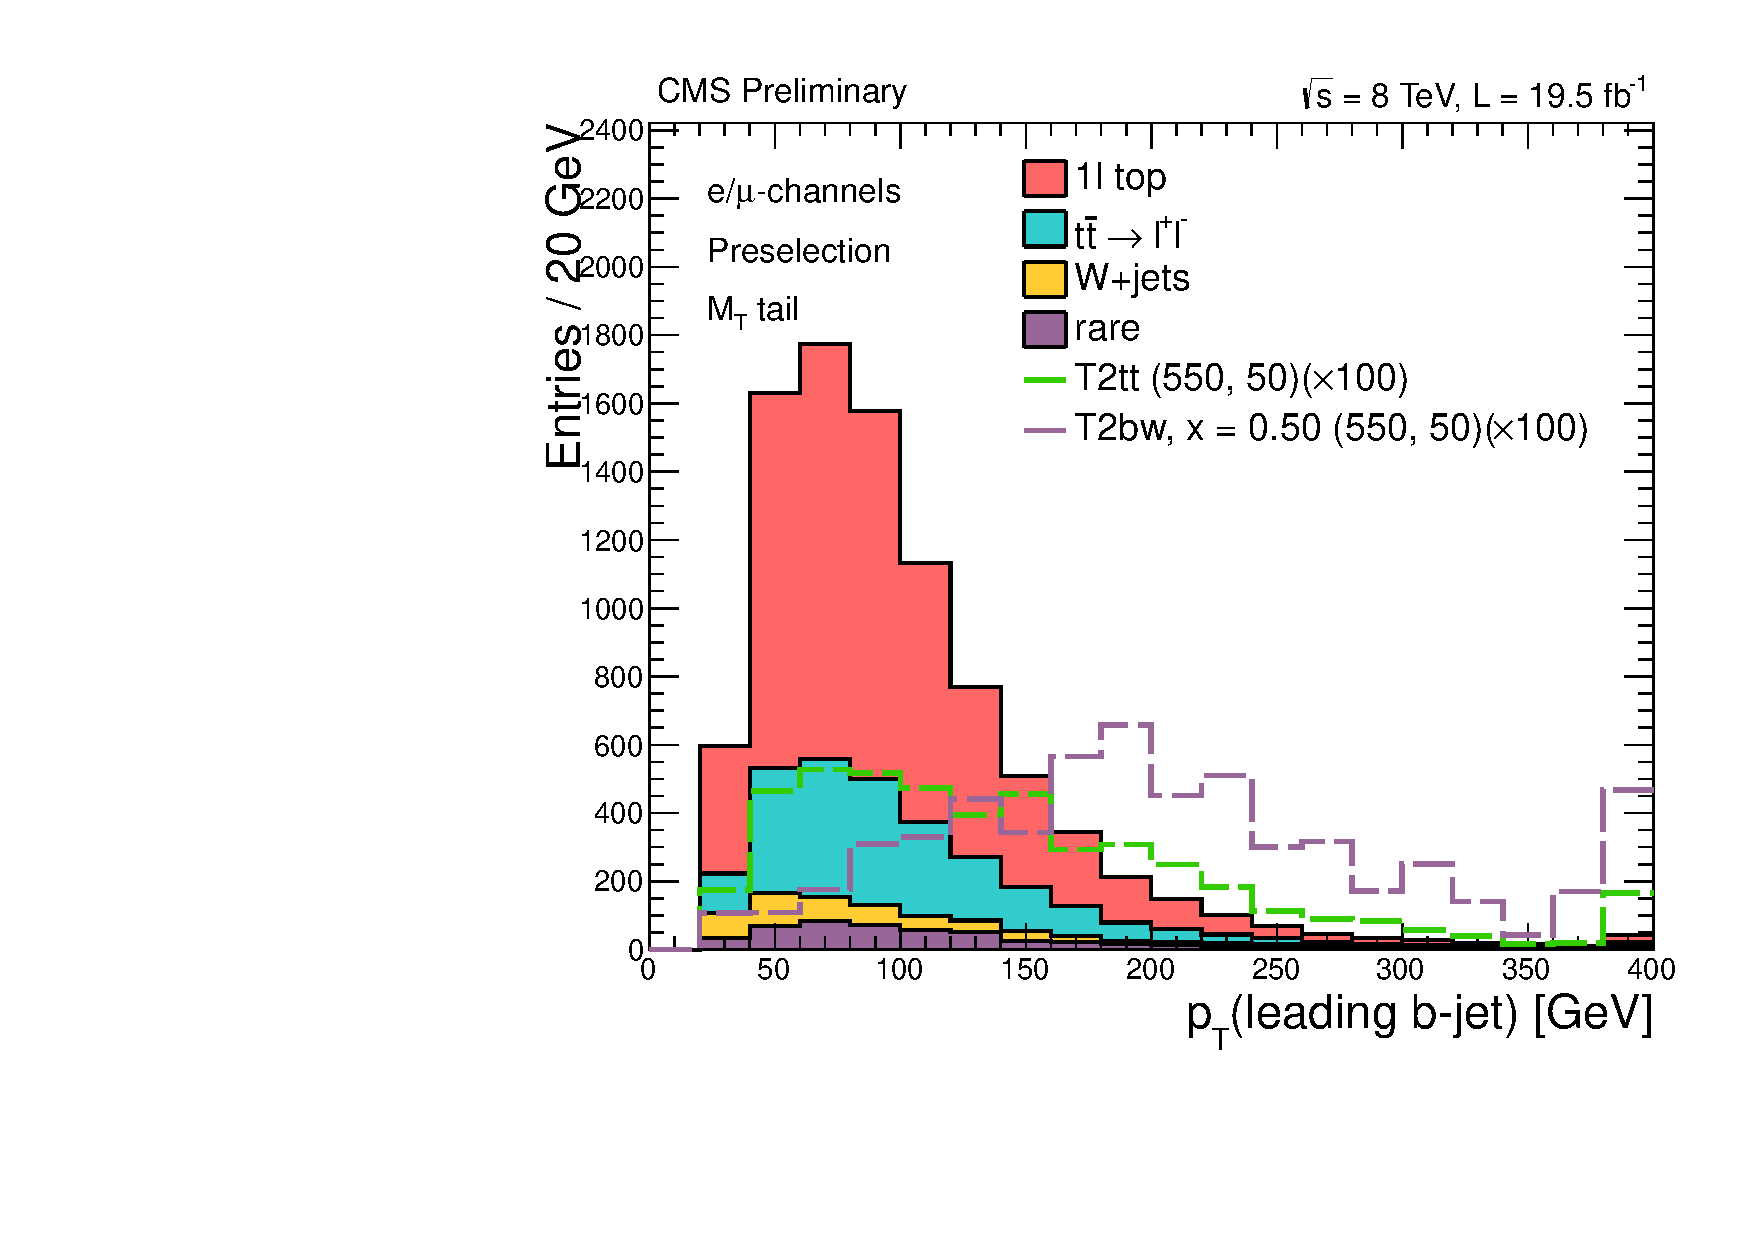
\includegraphics[width=0.32\textwidth]{variables/leadingBPt}
                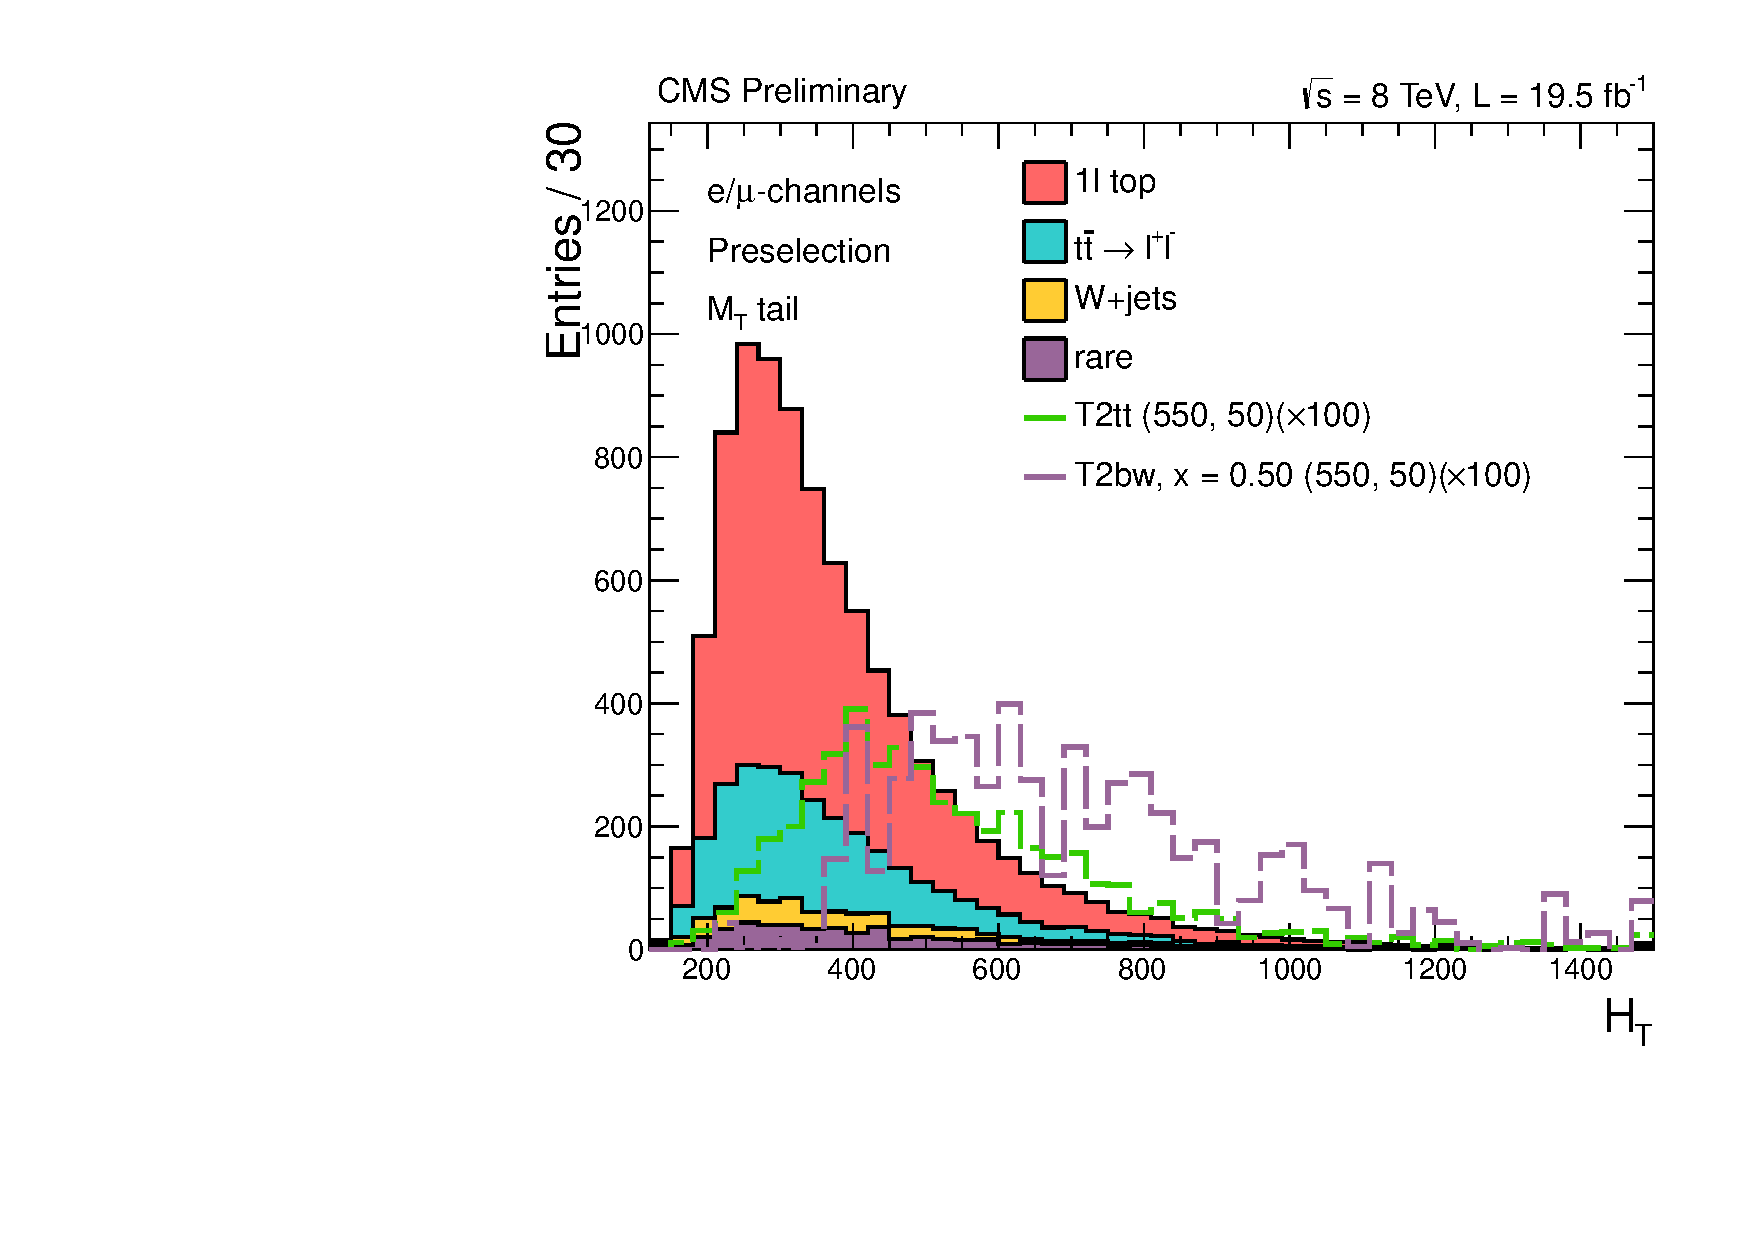
\includegraphics[width=0.32\textwidth]{variables/HT}
                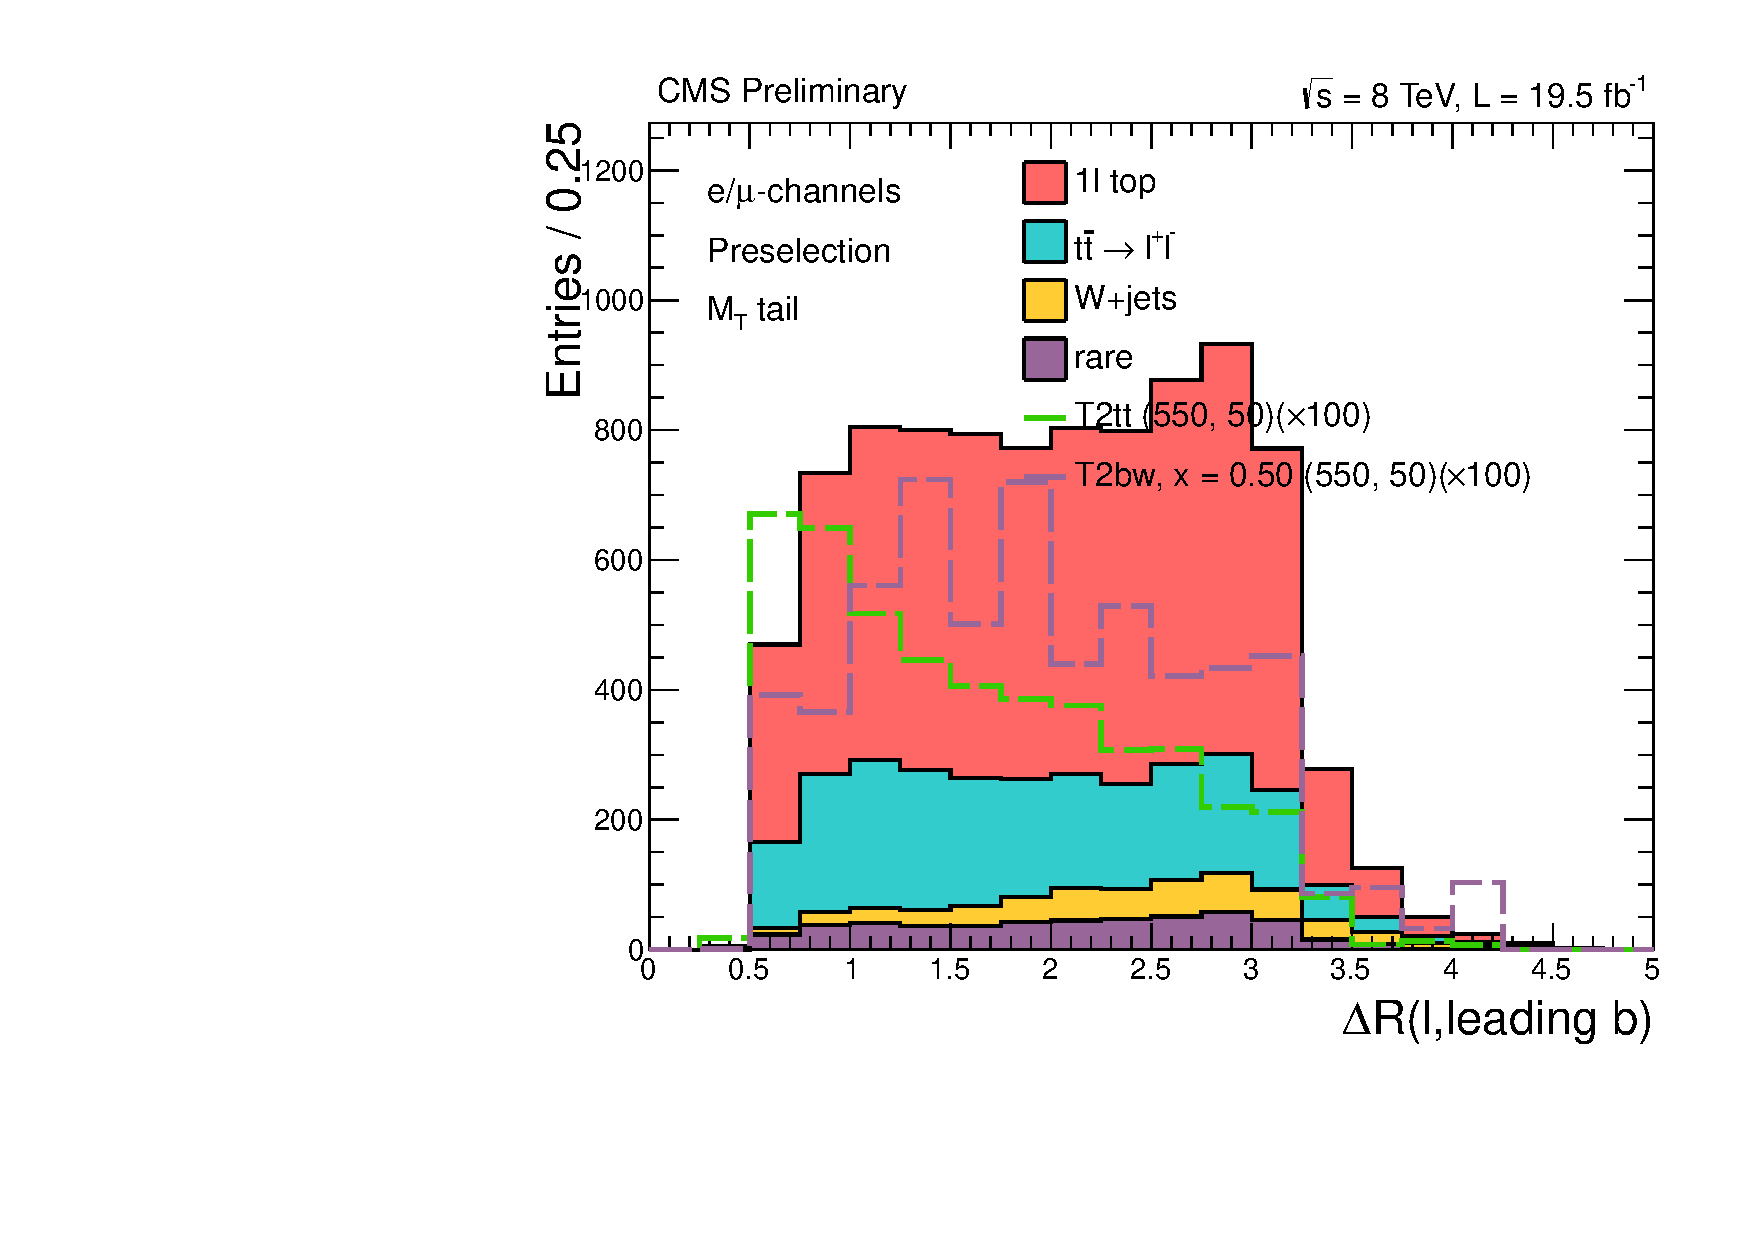
\includegraphics[width=0.32\textwidth]{variables/deltaRLeptonB}\\
                \includegraphics[width=0.32\textwidth]{variables/MET}
                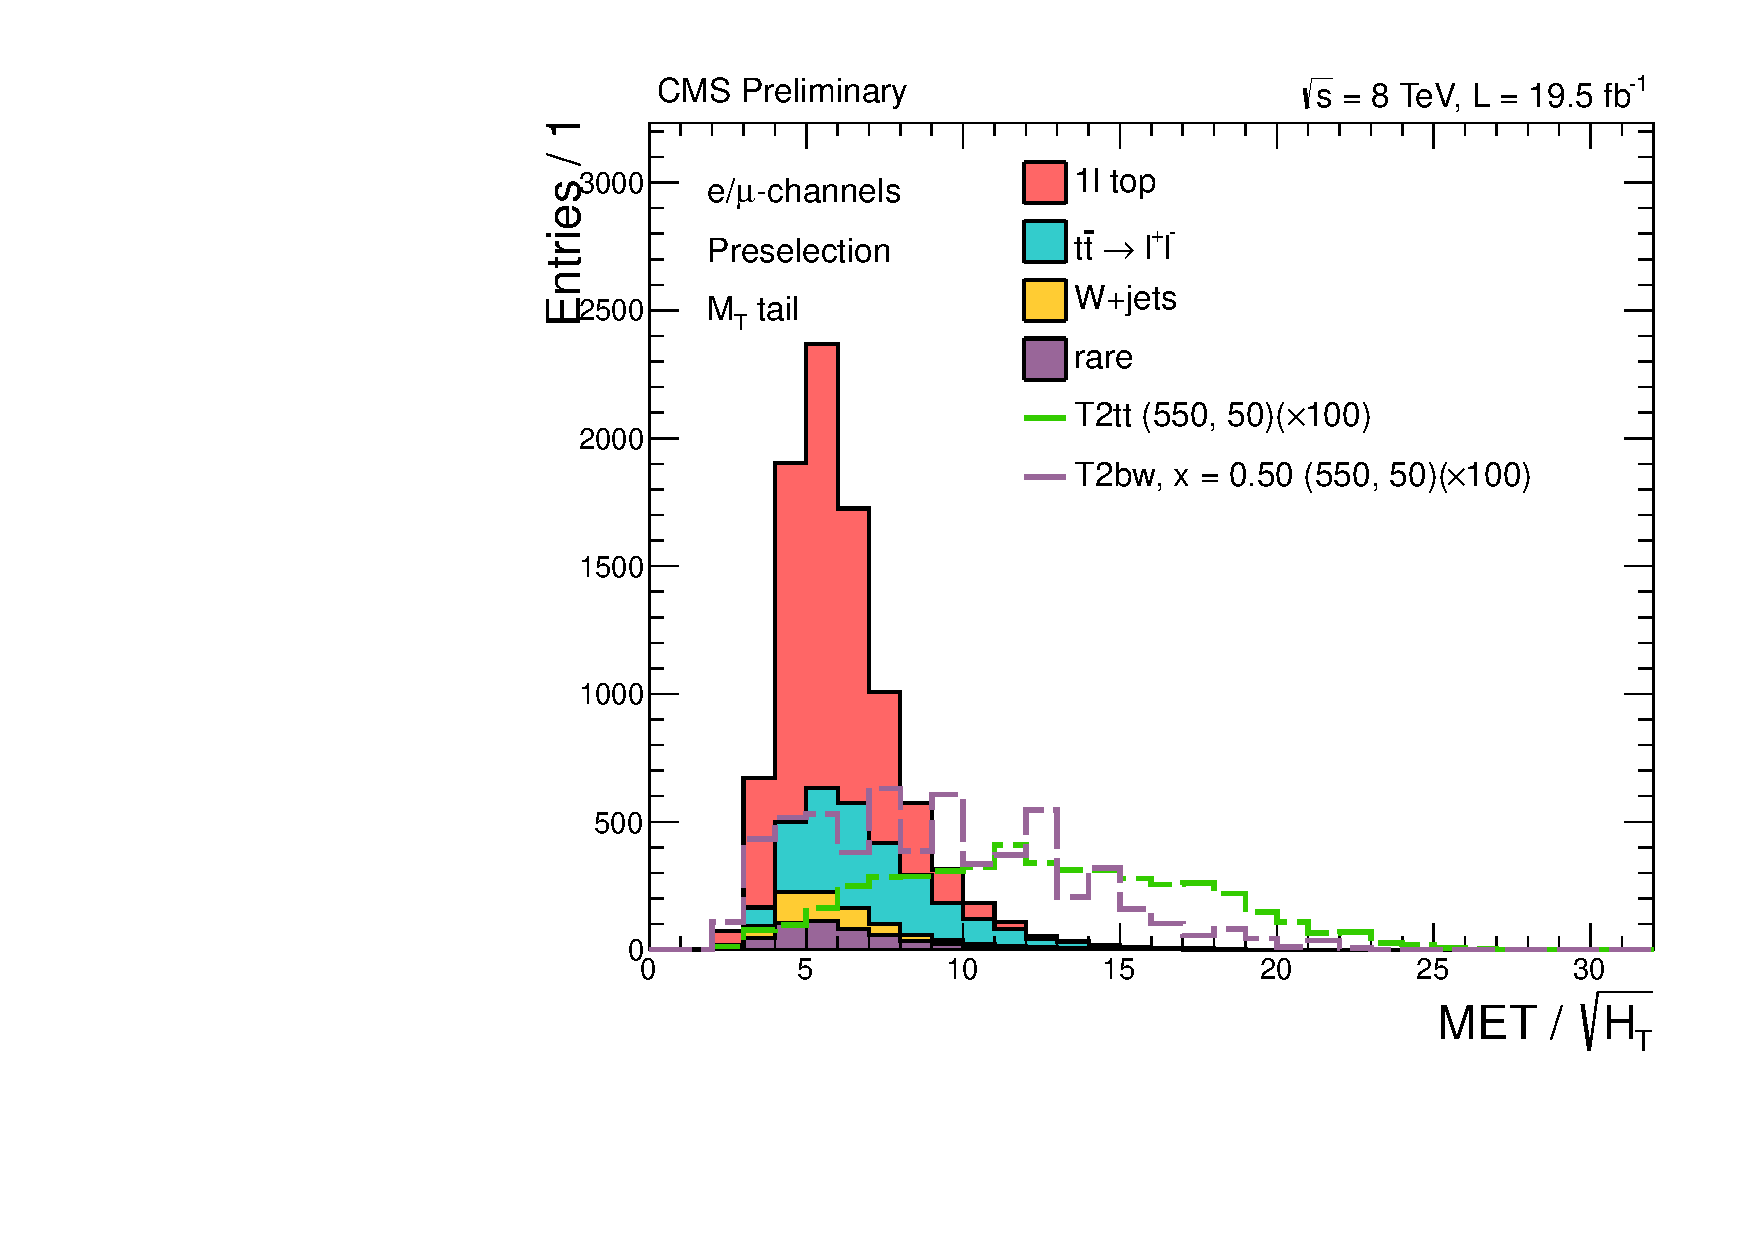
\includegraphics[width=0.32\textwidth]{variables/METoverSqrtHT}
                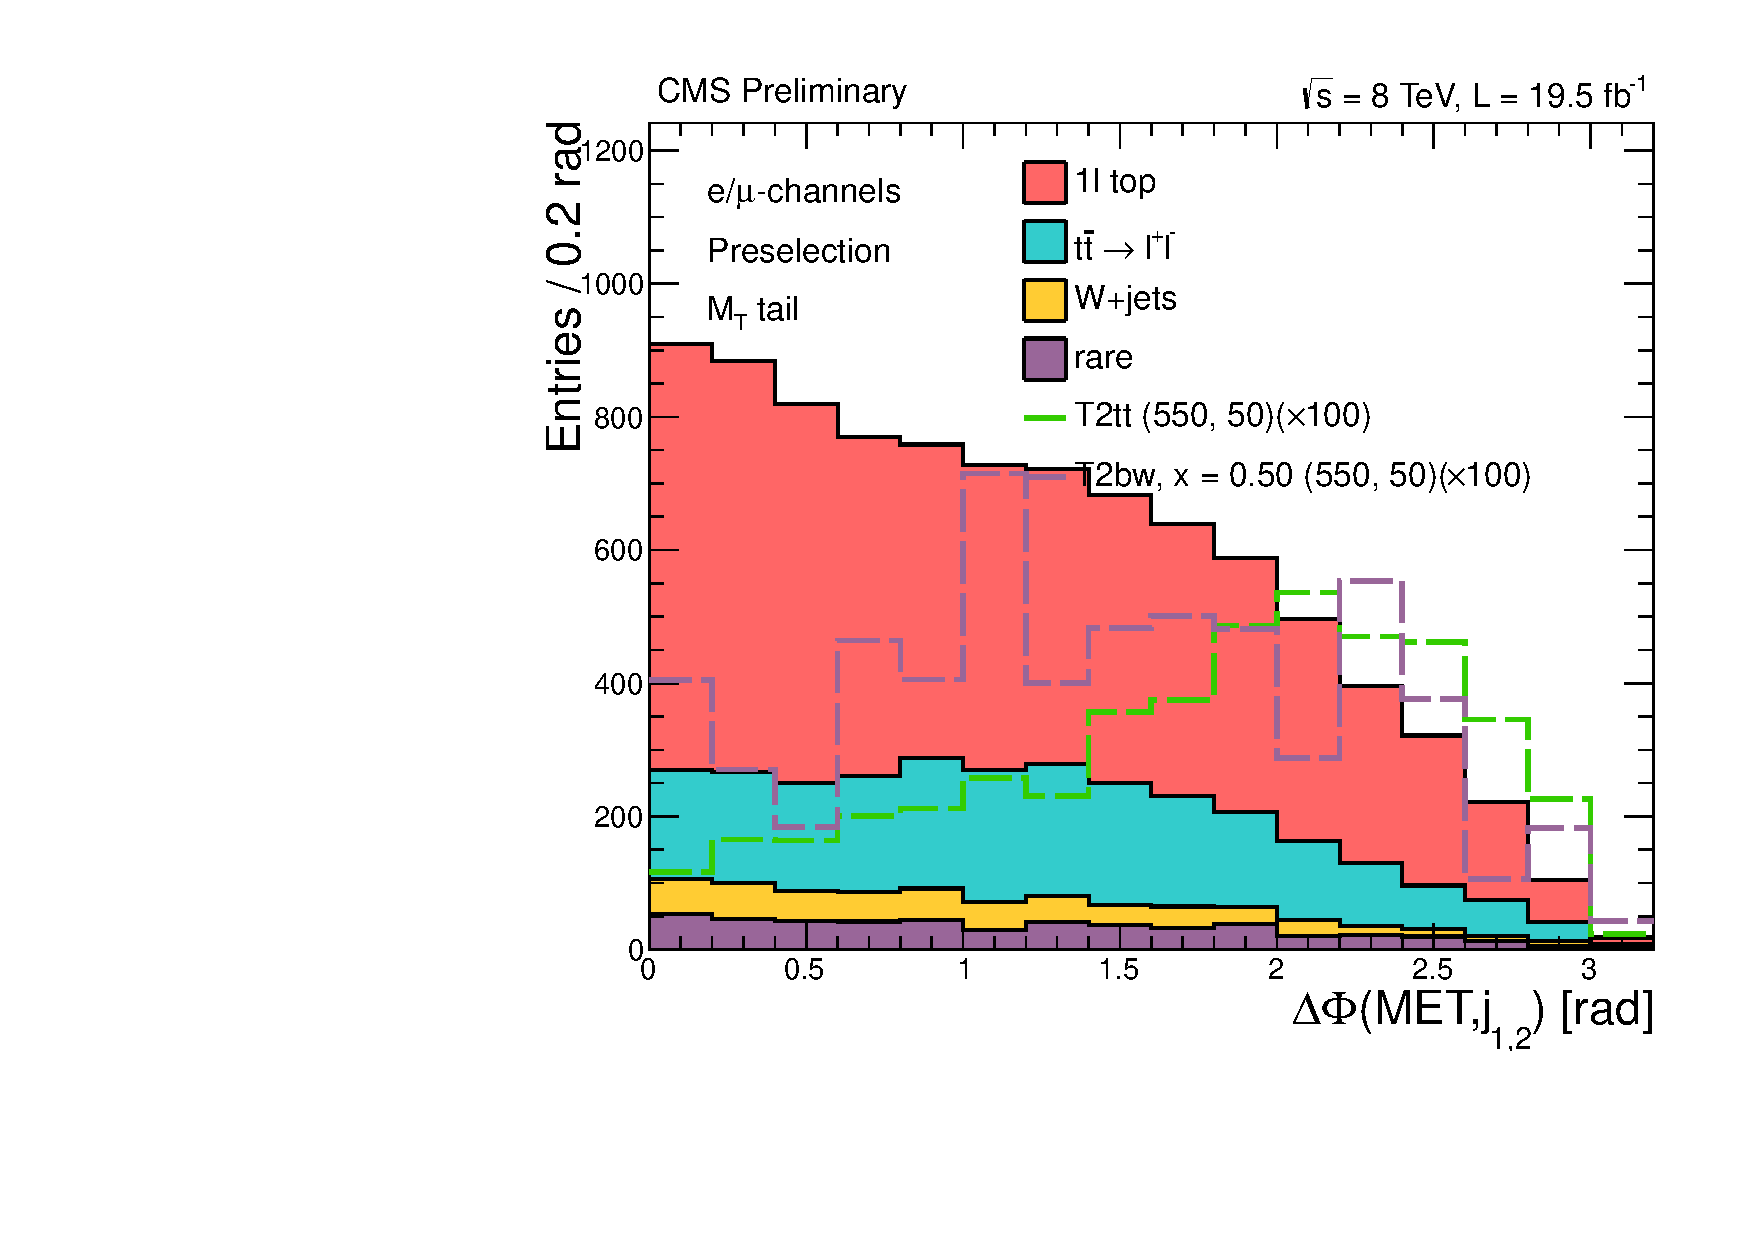
\includegraphics[width=0.32\textwidth]{variables/deltaPhiMETJets}\\
                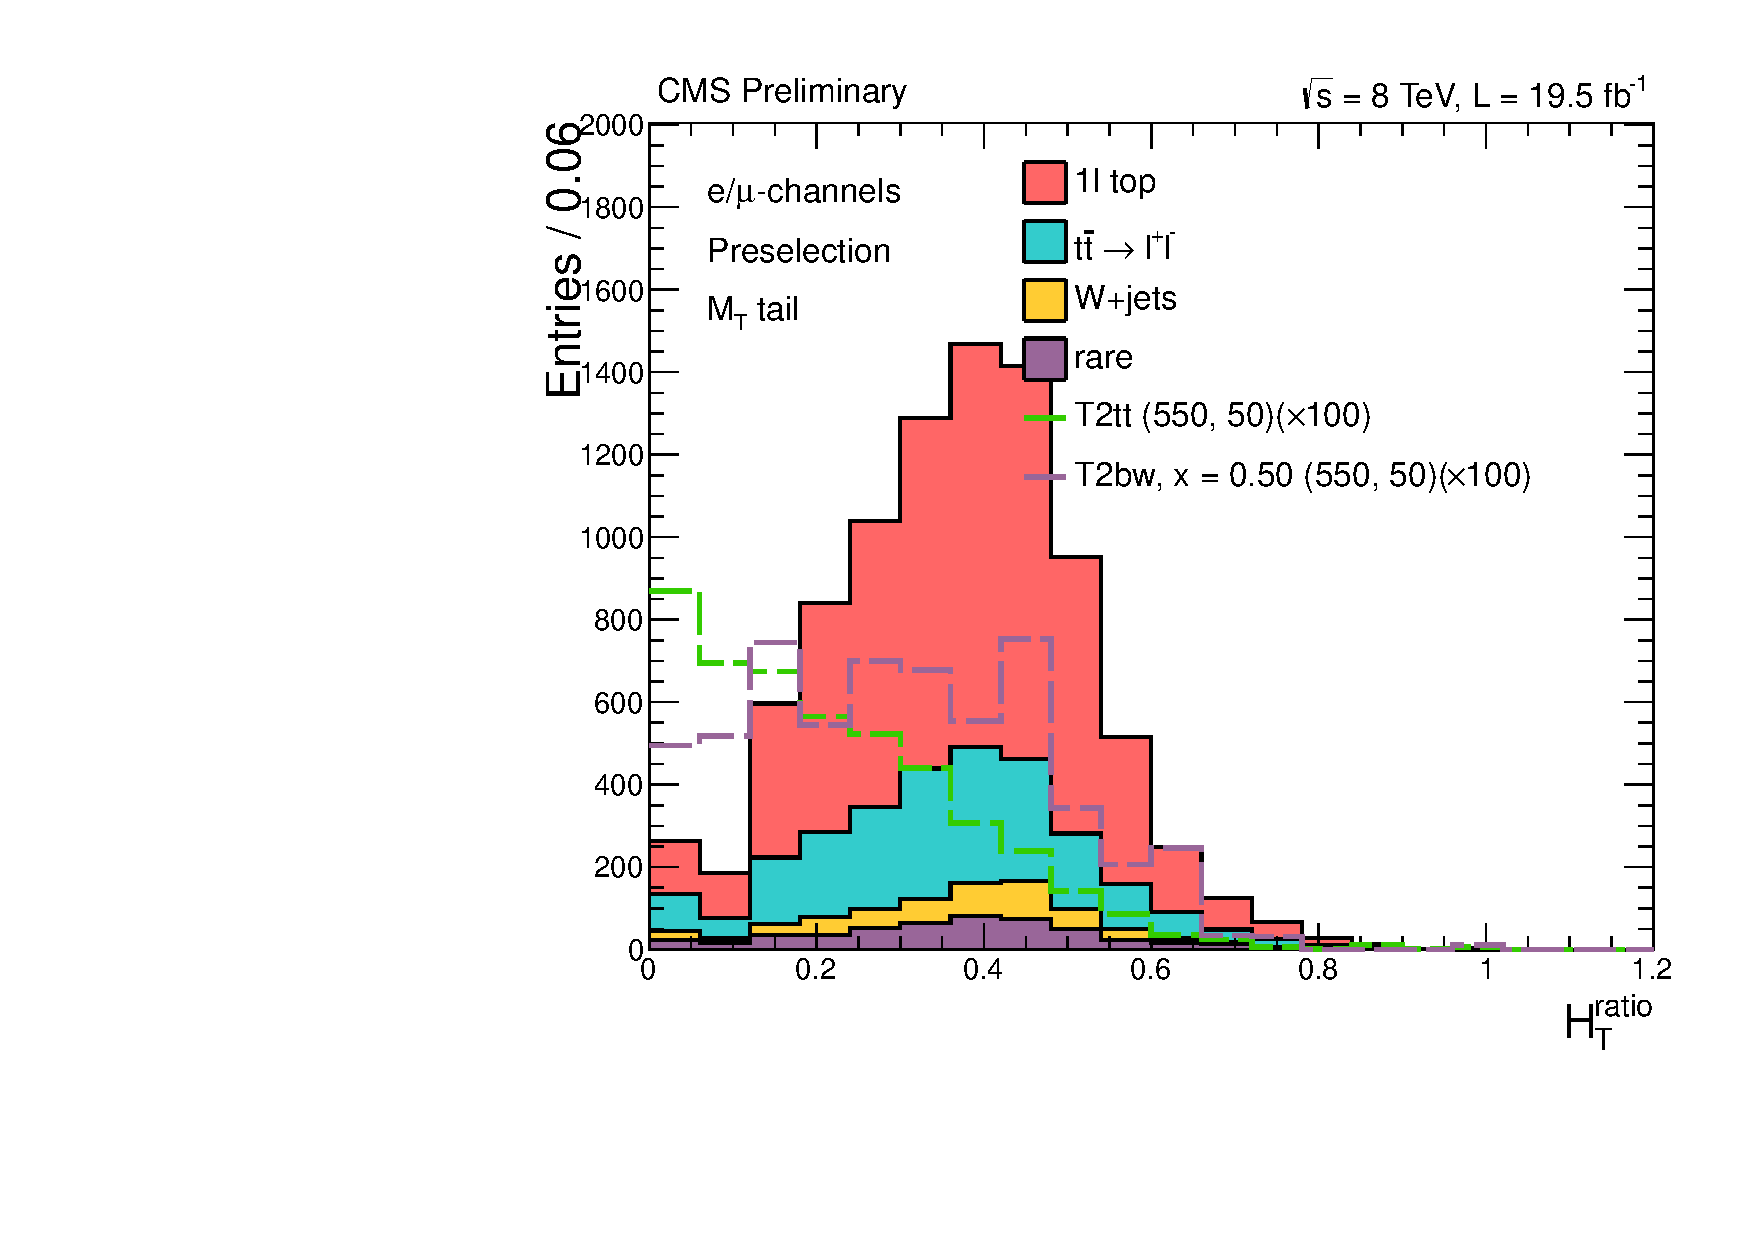
\includegraphics[width=0.32\textwidth]{variables/HTratio}
                \includegraphics[width=0.32\textwidth]{variables/MT2W}
                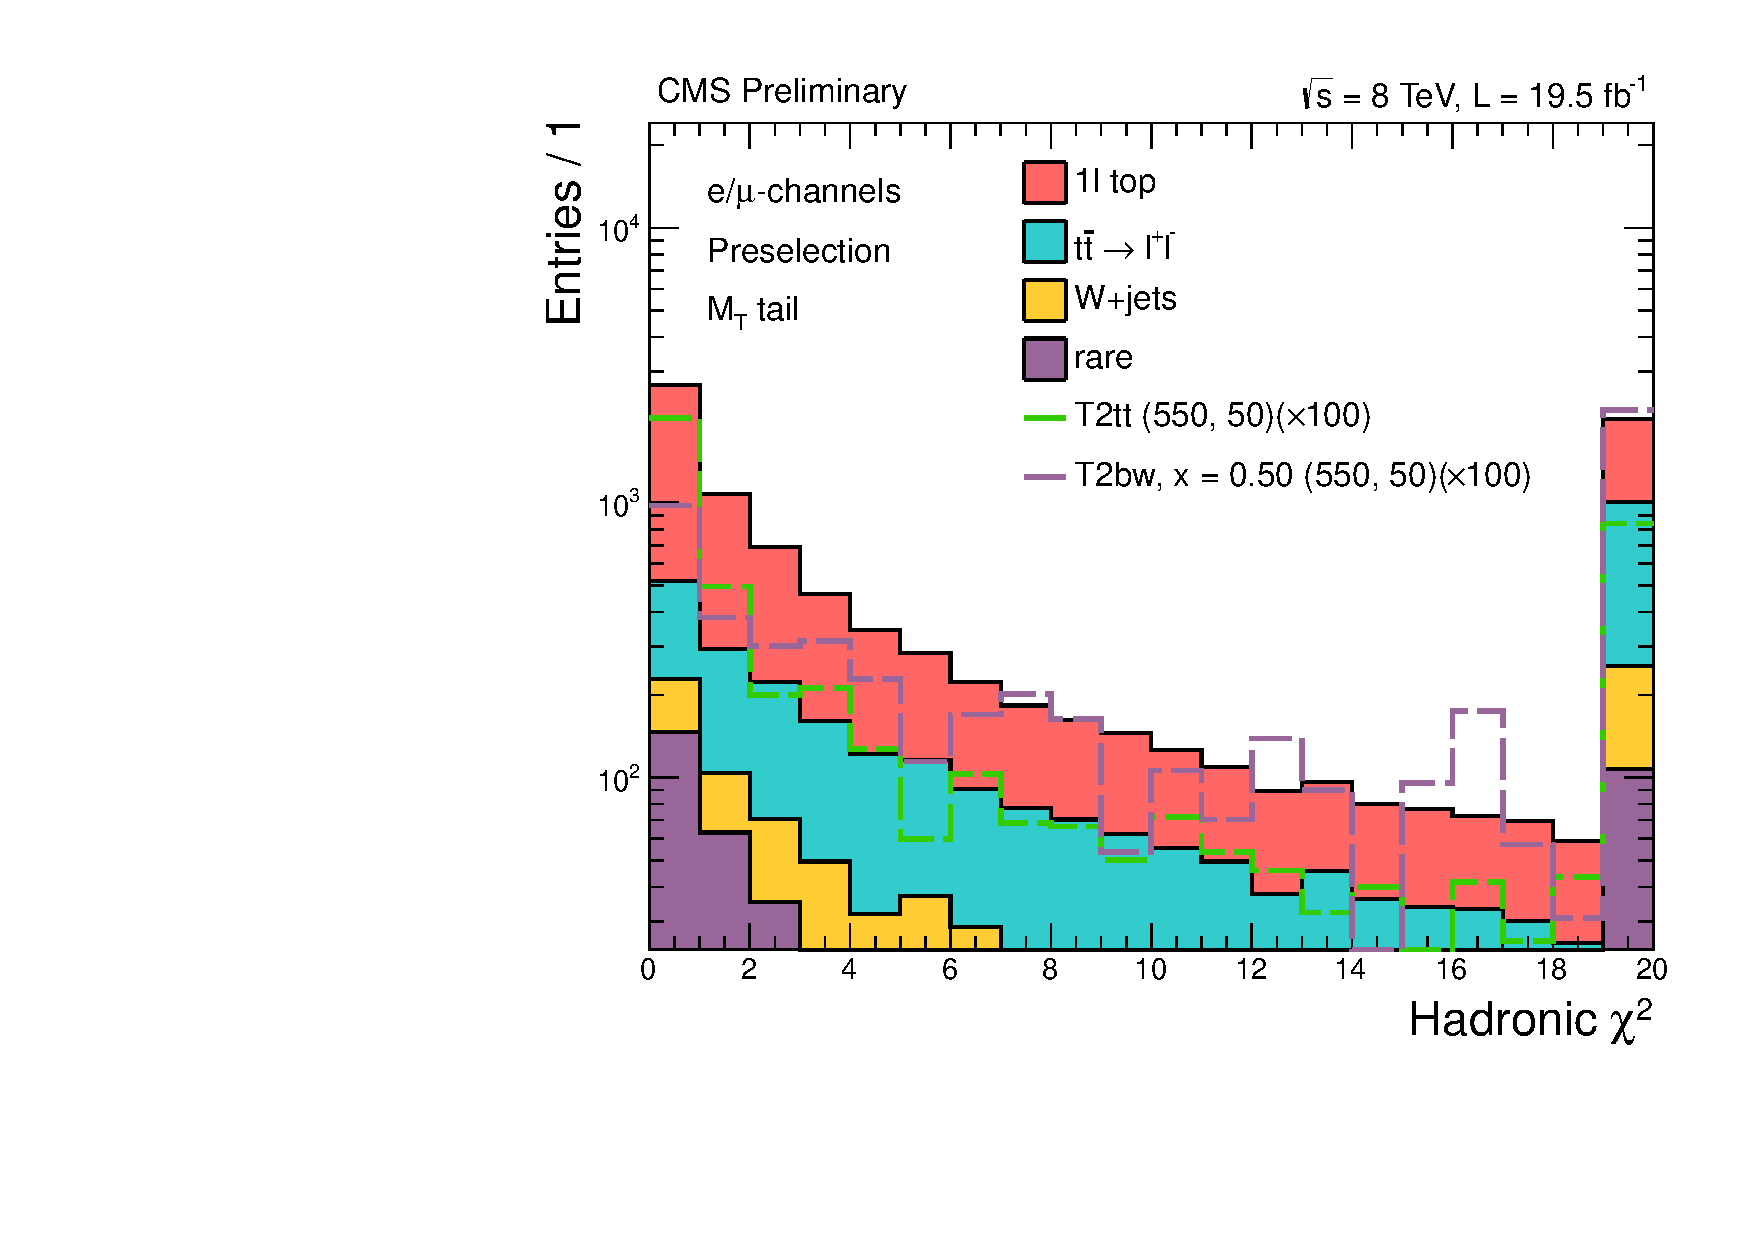
\includegraphics[width=0.32\textwidth]{variables/HadronicChi2}\\
                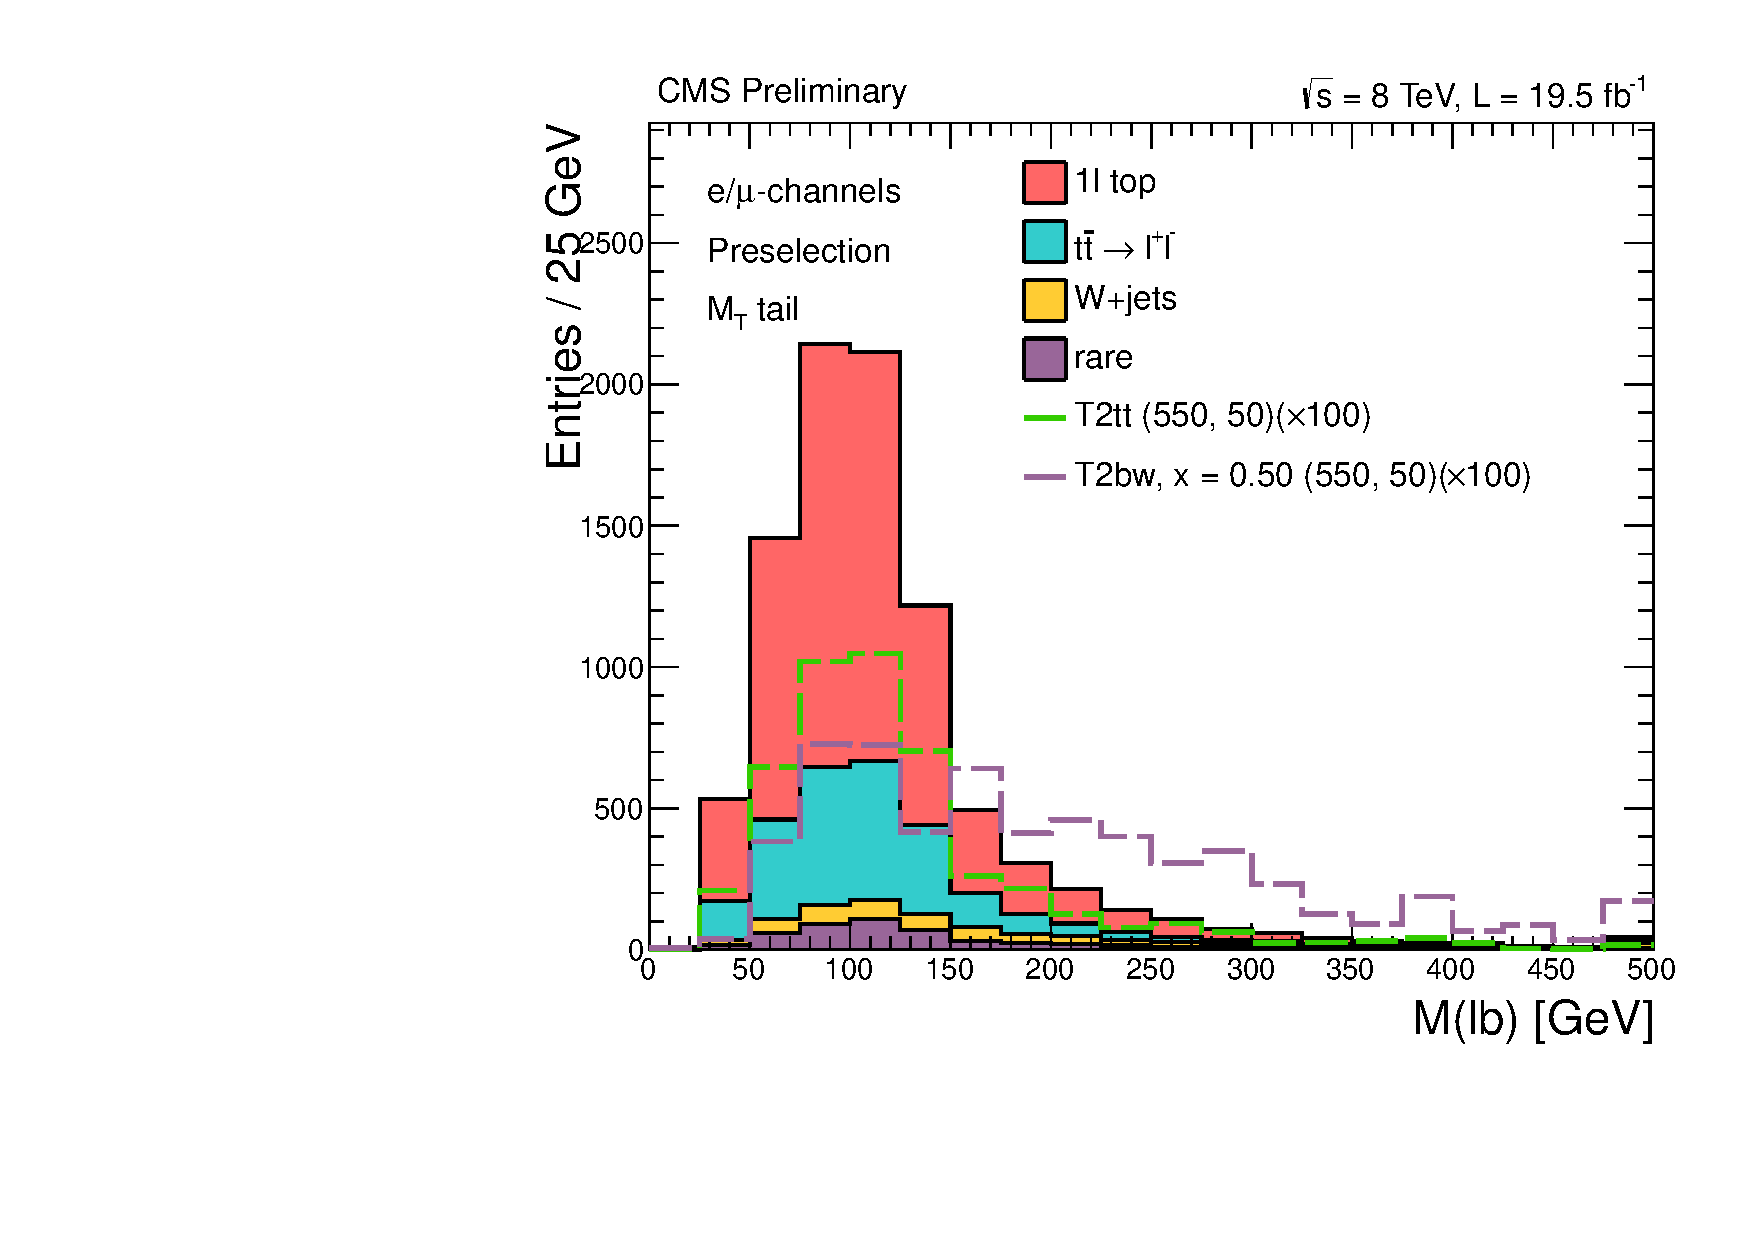
\includegraphics[width=0.32\textwidth]{variables/Mlb_hemi}
                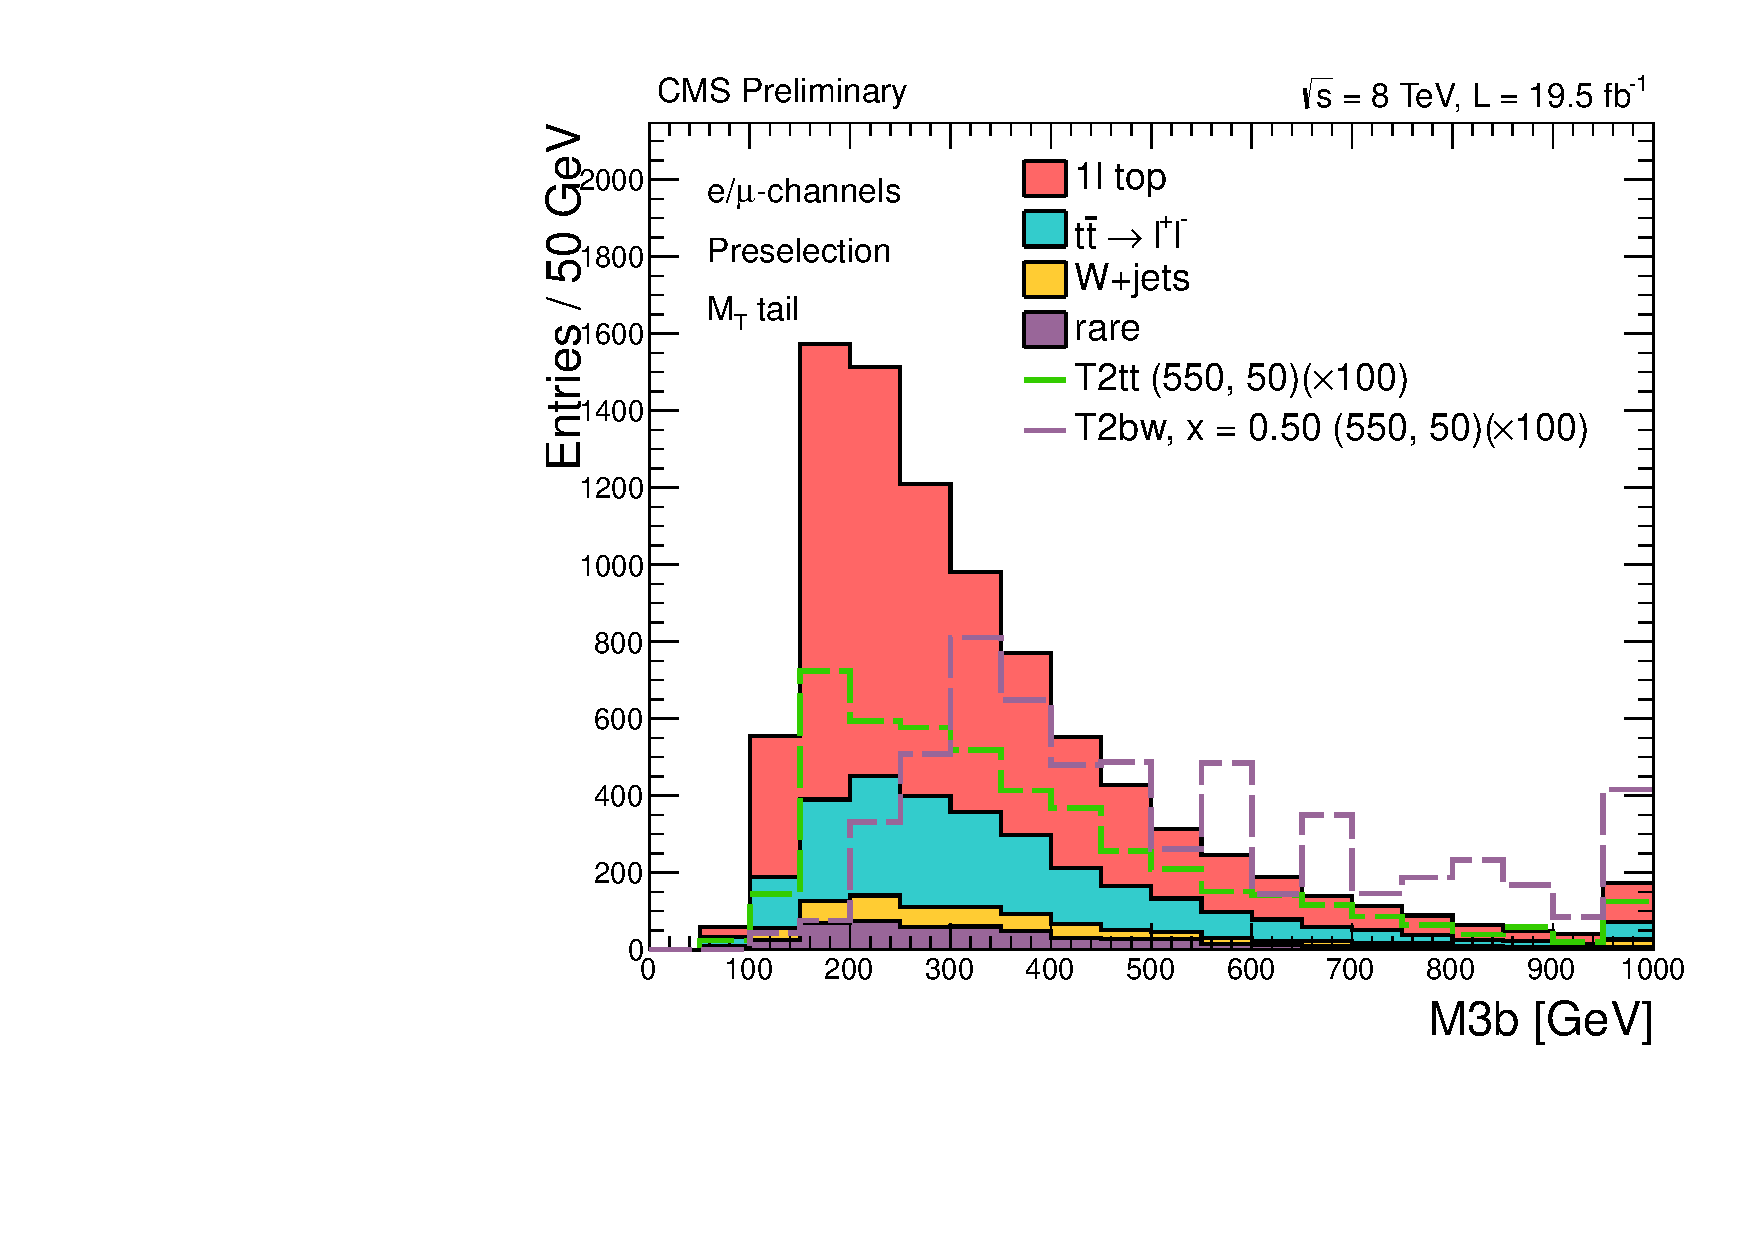
\includegraphics[width=0.32\textwidth]{variables/M3b}
                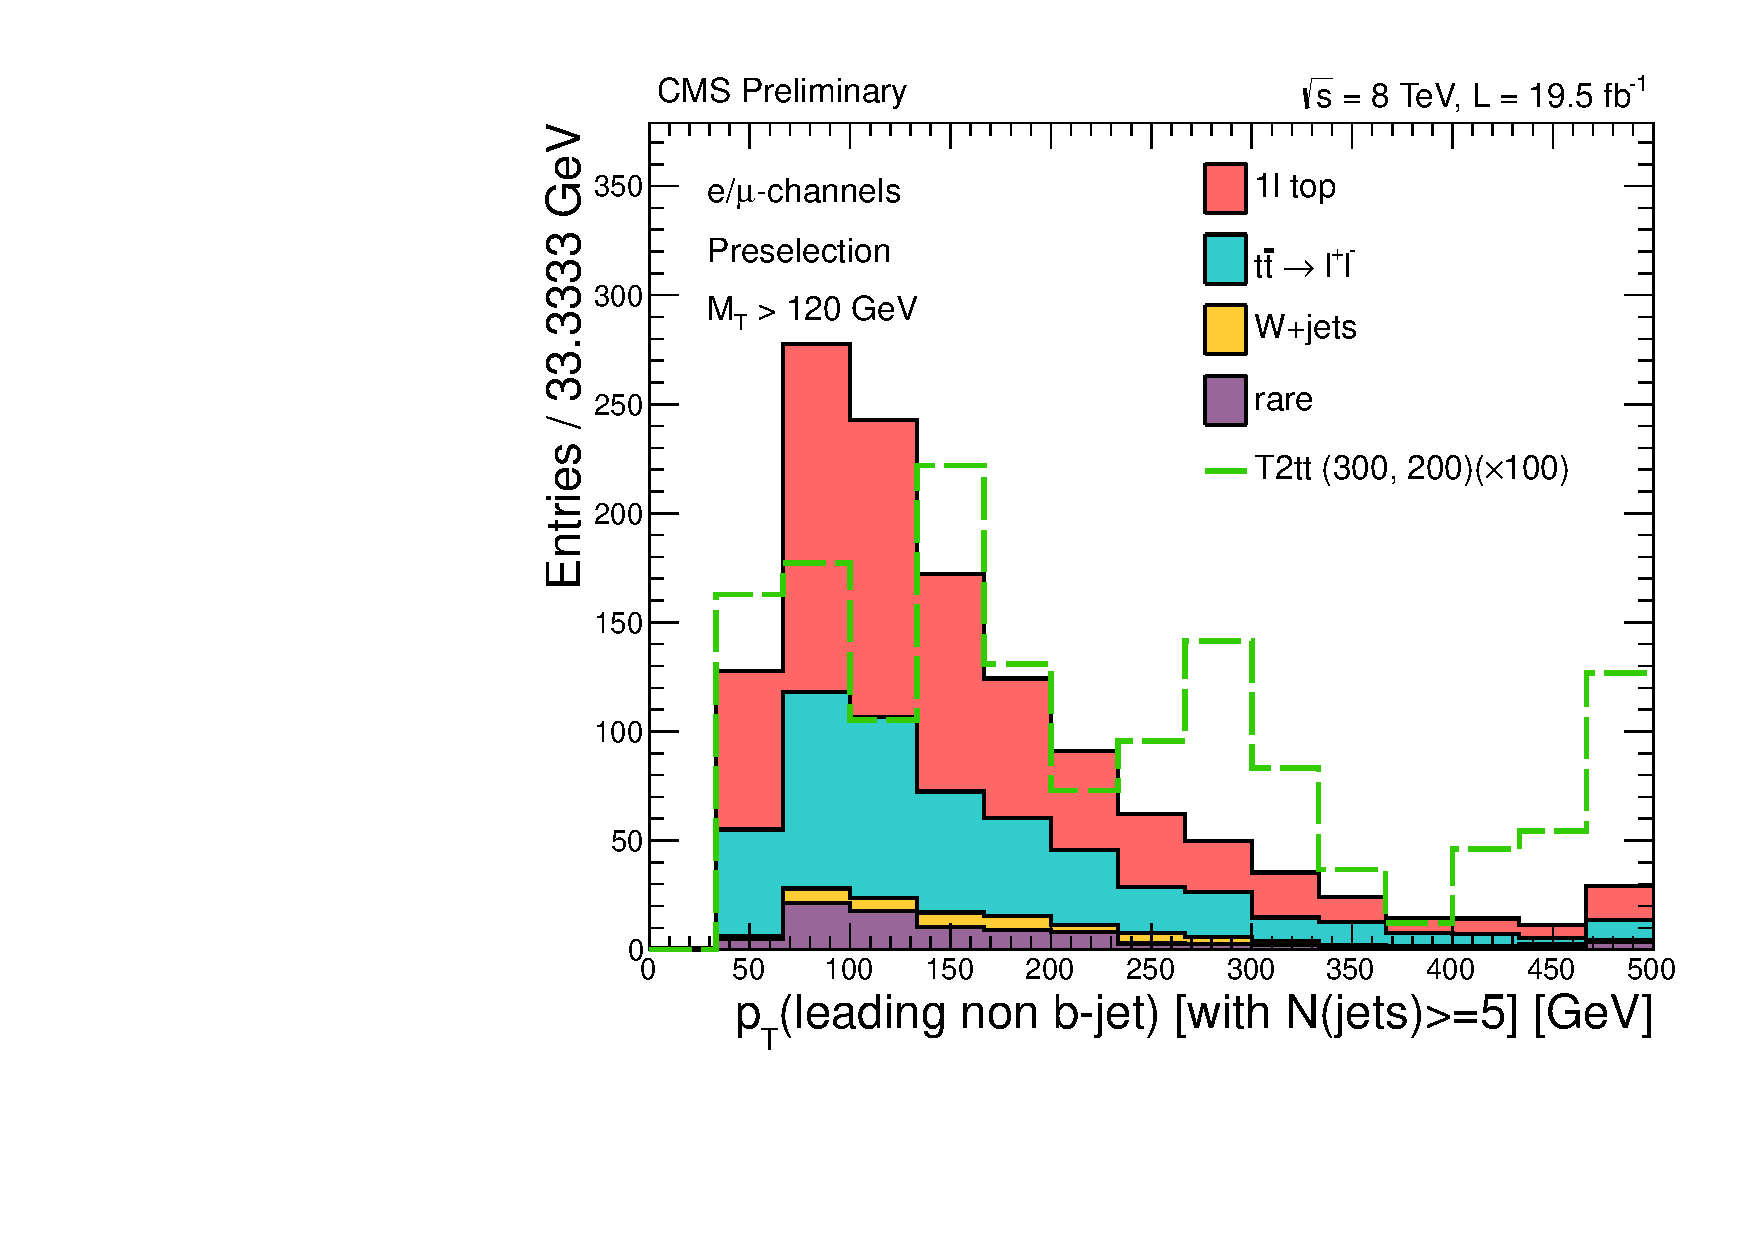
\includegraphics[width=0.32\textwidth]{variables/leadingNonBPtN5}
                \caption{Stacked plots representing the different discriminating variables used to design the signal region, for background and two signal examples after preselection and cut on $M_T > 100 \GeV$.
                \todo{update plot with missing variables and/or use same benchmark as previously, ie 450/50}}
                \label{fig:variables}
            \end{figure}

            \subsection{Figure of merit and sensitivity estimation}
            %==============================================================

    Before going into the details of the signal region optimization, we first need to
    introduce the metric used to do so. The problem of defining cuts to be applied on a
    variable can be summarized as knowing how to compromise between the quantity of
    selected signal, $S(\text{cut})$, versus selected background, $B(\text{cut})$, such
    that the sensitivity of the analysis is maximized. Ideally, one would run the full
    statistical interpretation which, in the context of the LHC experiments, is based
    on the $CL_S$ approach \refNeeded. However, such a procedure is CPU intensive as it is
    requires toy-data generation, and not suitable for a highly iterative process such
    as scanning possible cuts. In the case of a single-bin counting experiment, a more
    flexible way is to use analytical formula, called figure of merit (FoM) that gives an
    immediate estimation of the senstivity of the counting experiment.

    Let's consider the background only hypothesis $H_0$, also called null hypothesis,
    and the signal hypothesis $H_1$. These hypothesis are modeled by a probability density
    function (pdf), describing the probability to observe $N$ events in the data, as
    sketched on Figure \ref{fig:interpretation}.

    \insertFigure{interpretation}{0.7}
                 {Illustration of the modelization of the hypothesis $H_0$ and $H_1$ with
                 Poisson distributions of means and standard deviations being respectively
                 $(B,\sqrt{B})$ and $(S+B,\sqrt{S+B})$. \todo{fix plot}}

    From the point of view of excluding the signal hypothesis, a statistical hypothesis
    test consists in computing the probability $p$ to observe less than $D$ events in the
    data under $H_1$, $p(N < D|H_1)$. If this probability is lower than a treshold
    $\beta$, one may exclude the signal hypothesis with a confidence level $1-\beta$. A
    common practice is to use a confidence level of 95\%, or $\beta = 5\%$. The exclusion
    potential of a counting experiment can be defined via the probability $p(N < E[H_0]|H_1)$,
    i.e. the probability to observe a background-like realization in the data, if the
    signal exist. It is sometimes more pratical to express this potential in term of a
    significance $\mathcal{S}$, that is to say by expressing the distance $E[H_0] -
    E[H_1]$ in terms of standard deviations $\sigma[H_1]$ :

    $$ \mathcal{S}_\text{exclu.} = \frac{E[H_0] - E[H_1]}{\sigma[H_1]}$$

    If $H_1$ follows a gaussian distribution, then one can reinterpret $\mathcal{S}$ in terms
    of gaussian probabilities, for instance $\mathcal{S} = 2$ as a probability $p\approx5\%$
    using the so-called 68-95-99.7 rule of thumb in statistics. Considering that $H_0$ and
    $H_1$ have means and standard deviations being respectively $(B,\sqrt{B})$ and
    $(S+B,\sqrt{S+B})$ as in Figure \ref{fig:interpretation}, one ends up with

    $$ \mathcal{S}_\text{exclu.} = \frac{S}{\sqrt{S+B}}$$

    The same reasonning can be applied to the point of view of a discovery claim, where
    one is interested in $p(N > E[H_1]|H_0)$, i.e. the probability to observe a
    signal-like realization in the data, if the signal doesn't exist. Assuming the situation
    sketched in \ref{fig:interpretation}, one obtains a significance

    $$ \mathcal{S}_\text{disc.} = \frac{S}{\sqrt{B}}$$

    This significance definition can be easily used as a figure of merit when optimizing
    cuts. The picture may be completed by incoporating systematic uncertainties on the
    background to $\sigma[H_0]$ and $\sigma[H_1]$, leading to :

    \begin{equation}
       \mathcal{S}_\text{disc.} = \frac{S}{\sqrt{B+f^2 \cdot B^2}}
       \hspace*{2cm}
       \mathcal{S}_\text{exclu.} = \frac{S}{\sqrt{S+B+f^2 \cdot B^2}}
       \label{FoM}
   \end{equation}

    where $f$ represents an estimate of the relative systematic uncertainty on the background.

    While this figure of merit sometimes gives a reasonnable estimate of the true
    sensitivity of a counting experiment, one should remane conscious of its caveats
    \cite{Punzi} :

    \begin{enumerate}
        \item The intepretation of it is not straightfoward as it does not tell the
              physicist what can be expected to be excluded or discovered
              for a given counting experiment. It remains a 'number of sigmas', not an
              expected excluded cross-section.
        \item The formula \ref{FoM} does not contain any constrain regarding the fact that
              the observed number of events will be an integer. It will favorize a situation
              with $0.1$ signal events and expected background of $10^{-5}$ over a
              situation with 10 signal events and 1 background event, despite the fact that
              the later will definetely bring more information.
        \item It ultimately relies on a gaussian approximation which can cause significant
              discrepancies with respect to an accurate computation of $p(N|H)$. For instance,
              The Poisson and Gaussian tail integrals are significantly different at low
              means. More specifically, $\mathcal{S}_\text{disc.}$ is known to overestimate
              the true significance while $\mathcal{S}_\text{exclu.}$ underestimates it.
              Figure \ref{fig:} shows a comparison of $S/\sqrt{B}$ versus an exact
              computation.
    \end{enumerate}

    Caveat \#1 can be adressed by reinterpreting $\mathcal{S}$ in terms of excludable
    (or discoverable) signal strength $\mu$ or cross-section $\sigma$. Replacing
    $S$ with $\epsilon \times \sigma \times \mathcal{L}$, and introducing the discovery
    and exclusion treshold $a$ and $b$ (typically set to 5 and 2) yields :

    \begin{equation}
        \mathcal{\sigma}_\text{disc.} = a \cdot \frac{\sqrt{B+f^2B^2}}{\epsilon \cdot \mathcal{L}}
       \hspace*{2cm}
       \mathcal{\sigma}_\text{exclu.} = \frac{b}{2} \times \frac{b + \sqrt{b^2 + 4 (B + f^2B^2)}}{\epsilon \cdot \mathcal{L}}
       \label{FoM2}
    \end{equation}

    where $\epsilon$ and $\mathcal{L}$ are the selection efficiency and luminosity.

    Caveat \#2 can be worked around by imposing a minimum number of background and signal
    events when computing the figure of merit, for replacing $B$ with $\text{max}(B,1)$
    and ignoring cases with a too low expected signal yields.

    Finally, to address \#3, Ref. \cite{Punzi}, proposes an empirical fit to adjust the
    shape of the FoM with the accurate computation, as function of the parameters
    of the FoM. Alternative significances based on other approaches of the problem also
    exist and are discussed and compared in \todo{arXiv:physics/0702156v4 and arXiv:physics/0312059}.
    Figure \ref{fig:FOMcomparison} shows one of them, sometimes reffered to as Asimov Z and based on a
    likelihood approach, compared to the exact computation.

    \insertFigure{FOMcomparison}
                 {0.5}
                 {(From \todo{arXiv:1007:1727}, comparison of $S/\sqrt{B}$,
                 Asimov Z significance (denoted $\sqrt{q_{0,A}}$) and the exact significance computation
                 as function of $B$ and for $S = 2$, $5$ and $10$.}

        \subsection{Cut-based signal regions}
        %==============================================================

            \subsubsection{Optimization procedure}
            %==============================================================

    To design the cut-based signal regions on the analysis, the variables are first
    classified by their individual discriminating power, estimated by taking the
    maximum FoM achievable on a few signal benchmarks when scanning the possible
    cuts. The most discriminating variables are found to be $\MT$, $\MET$,
    $\MET/\sqrt{H_T}$ and $M_{T2}^{W}$. The variables $\Delta \phi(j_{1,2},\vec{\MET})$,
    hadronic top $\chi^2$, $\pT(\text{lead. } b)$ and the 5th, ISR jet requirement are
    also found to be helpful in particular cases or after cutting on the more discriminant
    variables. However we found that variables such as $H_T^\text{ratio}$, $M_{3b}$ and
    $M_{\ell b}$ offer lower potential.

    On a few signal benchmarks, we then proceed to a $n$-dimensionnal optimization of the
    cuts on these variables. We however impose some constrain in the use of the variables.
    First, either $\MET$ or $\MET/\sqrt{H_T}$ should be used, but not both at the same time.
    We allow tighter cuts on $\MT$ compared to the starting point $> 120\GeV$, but not
    tighter than $> 140\GeV$ especially to keep enough statistics for the background
    estimation related aspects.

    The optimization of the cuts is done with respect to the exclusion-oriented figure of
    merit defined in formula \ref{FoM}. To work around cases with very low background or signal leading,
    i.e. caveat \#2, we use $\tilde{B} \definedAs \text{max}(B,1)$ and set the FoM to 0
    if $S < 3$. The relative systematic uncertainty on the background is set to vary between
    15 and 30\% depending on the tightness of the cuts. We also incorporate some feedback
    of the background estimation that will be described later, by rescaling the $\oneLeptonTop$
    and $\Wjets$ contributions with a factor 1.3. This has for effect to favorize the
    rejection of these backgrounds over the $\diLeptonTop$ and rare components.

    After optimizing on a limited bunch of benchmarks, we inject all the sets of cuts found
    and map across the whole $(\mass{\lstop},\mass{\lneutralino)}$ space which is the one
    most performing set for each benchmark. As at this stage the number of set of cuts is
    large, and for the sake of keeping things manageable, we aim to reduce this number by
    manually clustering similar sets while keeping sure to not significantly loose in
    terms of performances.

            \subsubsection{Results and performances}
            %==============================================================

    The resulting signal regions definitions are presented on Table \ref{tab:cutAndCountCuts}.
    As announced in section \ref{sec:analysis_variables}, $\MET/\sqrt{H_T}$ tends to be
    preferred at low $\deltam$ compared to $\MET$. In the off-shell and stealthy regime,
    the ISR jet requirement plays an important role to gain sensitivity, despite the
    fact that this leaves little room for other cuts given the already low preselection
    efficiency and the tightness of requiring a 5th jet at high $p_T$.
    In the medium and high $\deltam$ regime, cutting on $M_{T2}^W$ provides a good gain
    in sensitivity because the large $\MET$ of the signal is less likely to decomposable
    in such a way that it fits the constrains while style yielding a light $m_Y$ mass.
    At low and medium $\deltam$ regimes for the $\lstop \rightarrow t \lneutralino$, the
    hadronic top $\chi^2$ provides a good alternative or complementary approach to $M_{T2}$
    for rejecting the $\diLeptonTop$ background. For $\lstop \rightarrow b \lchargino$,
    at low and medium $x$, the $\pT$ of the leading $b$ is an important feature, related
    to the high $\lstop-\lchargino$ gap. Finally, in almost all signal regions,
    $\Delta\phi(j_{1,2},\vec{\MET})$ proves to be useful by providing a way to reject the
    $\oneLeptonTop$ component where $\vec{\MET}$ is expected to be close to a ($b$-)jet.

    Figure \ref{fig:cutAndCountPerformances} shows the best performing set accross the
    $(\mass{\lstop},\mass{\lneutralino})$ plane as well as the corresponding FoM. While
    these results are purely based on the FoM, the final choice of the signal region to
    be used for each benchmark later done by choosing the minimum expected cross-section
    upper limit from the $CL_s$ computation.

\begin{table}[!ht]
{\footnotesize
\begin{center}
\hspace*{-0.8cm}
    \begin{tabular}{|l|ccccccc|}
    \hline
    $\lstop \rightarrow t\lneutralino$ & $\MT$   & $\MET$    & $\MET/\sqrt{H_T}$  & $M_{T2}^W$ & Hadronic top $\chi^2$ & $\Delta\phi(j_{1,2},\vec{\MET})$      &   5th, ISR jet \\
    \hline
    1) off-shell (loose)       & $>$ 125 & -       &   $>$ 8            &     -     & -             &          - &    yes        \\
    2) off-shell (tight)       & $>$ 130 & $>$ 300 &   -                &     -     & -        	    &          - &    yes        \\
    3) low    $\mass{\lstop}$  & $>$ 140 & -       &   $>$ 8            &     -     &  $<$ 5        &  $>$ 0.8   &    -          \\
    4) medium $\deltam$        & $>$ 140 & $>$ 200 &   -                &  $>$ 180  &  $<$ 3        &  $>$ 0.8   &    -          \\
    5) high   $\deltam$        & $>$ 130 & $>$ 350 &   -                &  $>$ 190  & -             &          - &    -          \\
        \hline
    \end{tabular}
    \hspace*{-0.5cm}
    \begin{tabular}{|l|ccccccc|}
    \hline
    $\lstop \rightarrow b\lchargino, x=0.25$   & $\MT$     & $\MET$    & $\MET/\sqrt{H_T}$ & $M_{T2}^W$ & $\pT(\text{lead. }b)$ & $\Delta\phi(j_{1,2},\vec{\MET})$ & 5th, ISR jet  \\
    \hline
    1) off-shell        & $>$ 120   &  -       &    $>$  9       &     -      &   -                   &  $>$ 0.2      & yes           \\
    2) low    $\deltam$ & $>$ 120   &  -       &    $>$  6       &  $>$ 200   & $>$ 180               &  $>$ 0.8      & -             \\
    3) high   $\deltam$ & $>$ 120   & $>$ 300  &     -           &  $>$ 200   & $>$ 180               &  $>$ 0.8      & -             \\
    \hline
    $\lstop \rightarrow b\lchargino, x=0.50$     & $\MT$     & $\MET$    & $\MET/\sqrt{H_T}$ & $M_{T2}^W$ & $\pT(\text{lead. }b)$ & $\Delta\phi(j_{1,2},\vec{\MET})$ & 5th, ISR jet  \\
    \hline
    1) off-shell        &  $>$ 120  &   -      &  $>$  9         &    -       & -                     &  $>$ 0.2      & yes           \\
    2) low masses       &  $>$ 135  &   -      &  $>$  6         & $>$ 180    & -                     &  $>$ 0.8      & -             \\
    3) medium $\deltam$ &  $>$ 140  &   -      &  $>$  7         & $>$ 190    & $>$ 100               &  $>$ 0.8      & -             \\
    4) high   $\deltam$ &  $>$ 120  & $>$ 300  &   -             & $>$ 200    & $>$ 100               &  $>$ 0.8      & -             \\
    \hline
    $\lstop \rightarrow b\lchargino, x=0.75$   & $\MT$     & $\MET$    & $\MET/\sqrt{H_T}$ & $M_{T2}^W$ & $\pT(\text{lead. }b)$ & $\Delta\phi(j_{1,2},\vec{\MET})$ & 5th, ISR jet  \\
    \hline
    1) low    $\deltam$ &  $>$ 120  &   -      &  $>$  12        &     -      &      -                &  $>$ 0.8      & yes           \\
    2) medium $\deltam$ &  $>$ 130  &   -      &  $>$  10        &  $>$ 180   &      -                &  $>$ 0.8      & -             \\
    3) high   $\deltam$ &  $>$ 140  & $>$ 300  &    -            &  $>$ 200   &      -                &  $>$ 0.8      & -             \\
    \hline
    \end{tabular}
\caption{Description of the signal regions defined and optimized for the cut-based approach. \label{tab:cutAndCountCuts}}
\end{center}}
\end{table}


            \begin{figure}[h!]
                \centering
                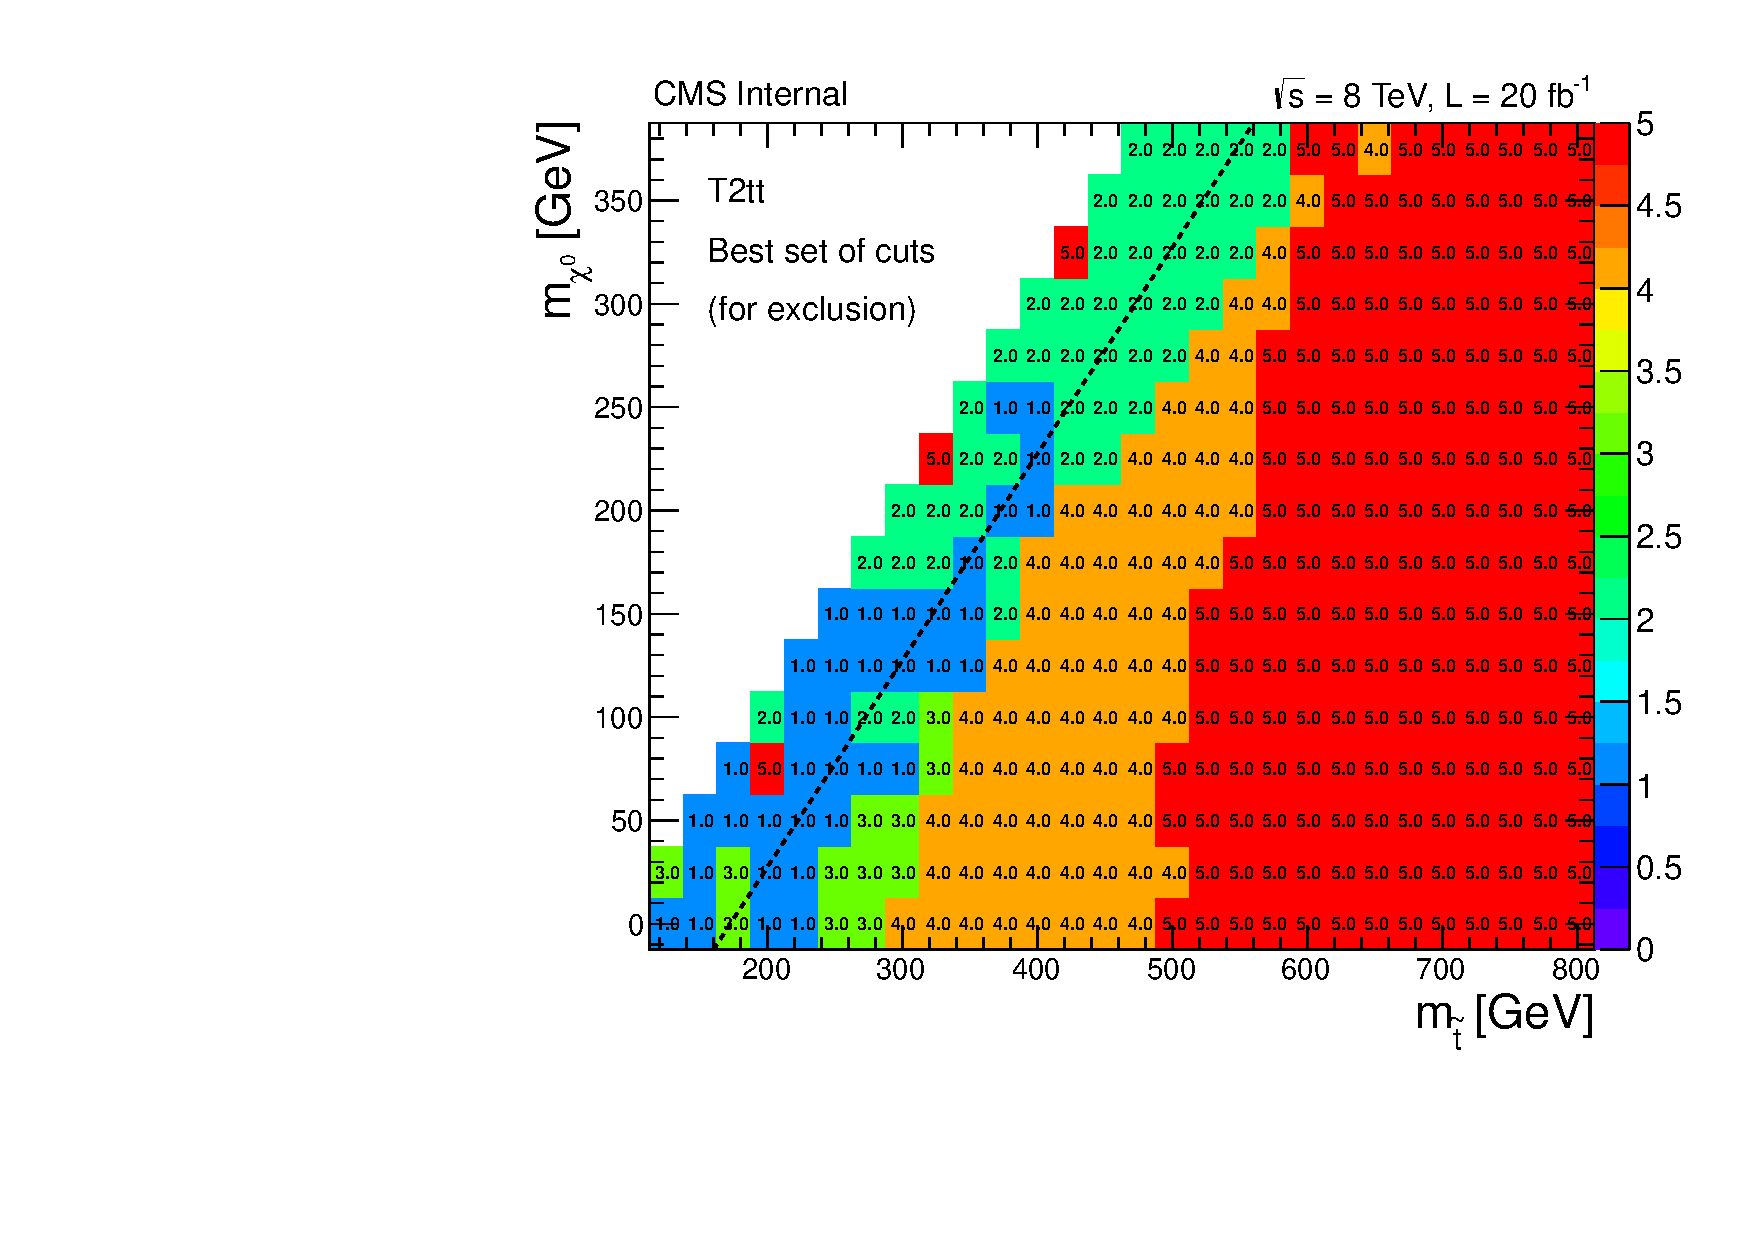
\includegraphics[width=0.37\textwidth]{cutAndCountPerformances/bestSet_T2tt}
                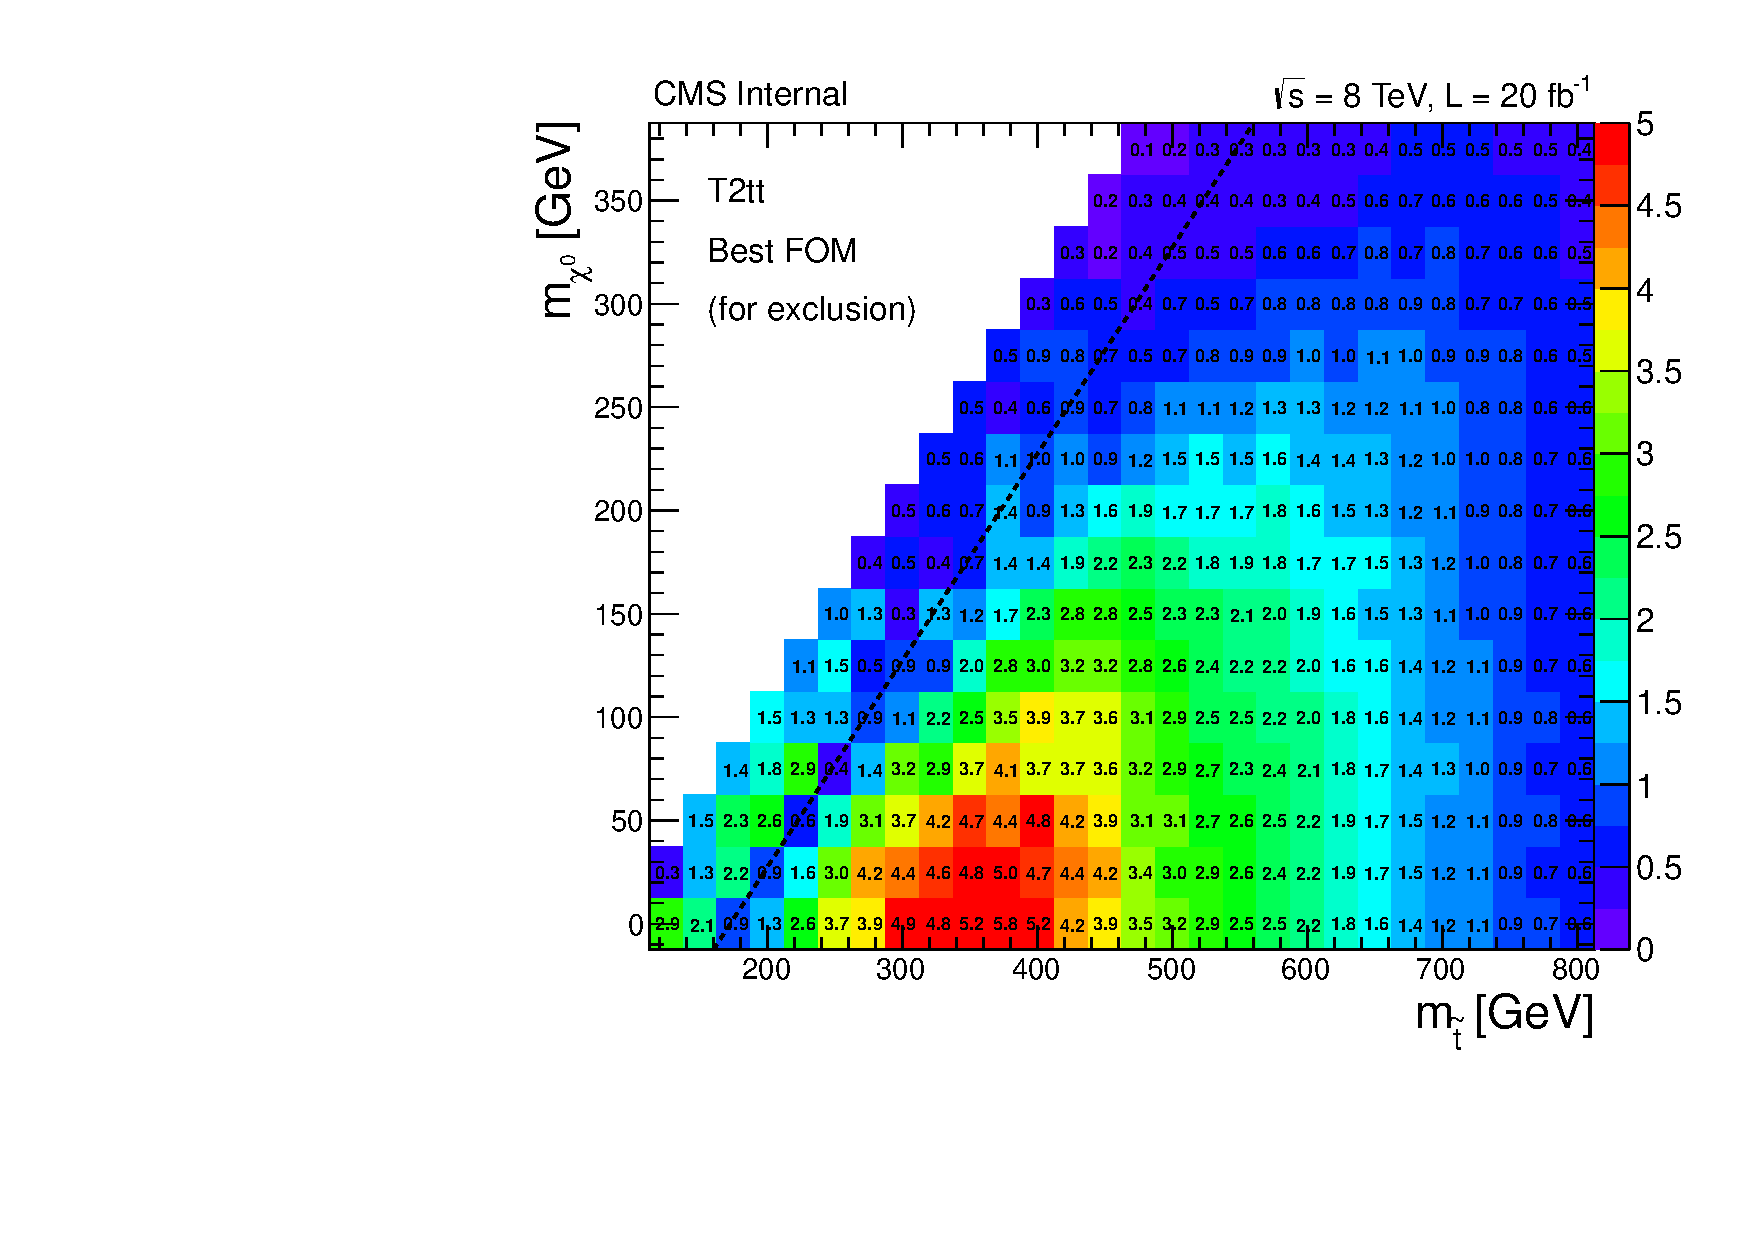
\includegraphics[width=0.37\textwidth]{cutAndCountPerformances/bestFOM_T2tt}\\
                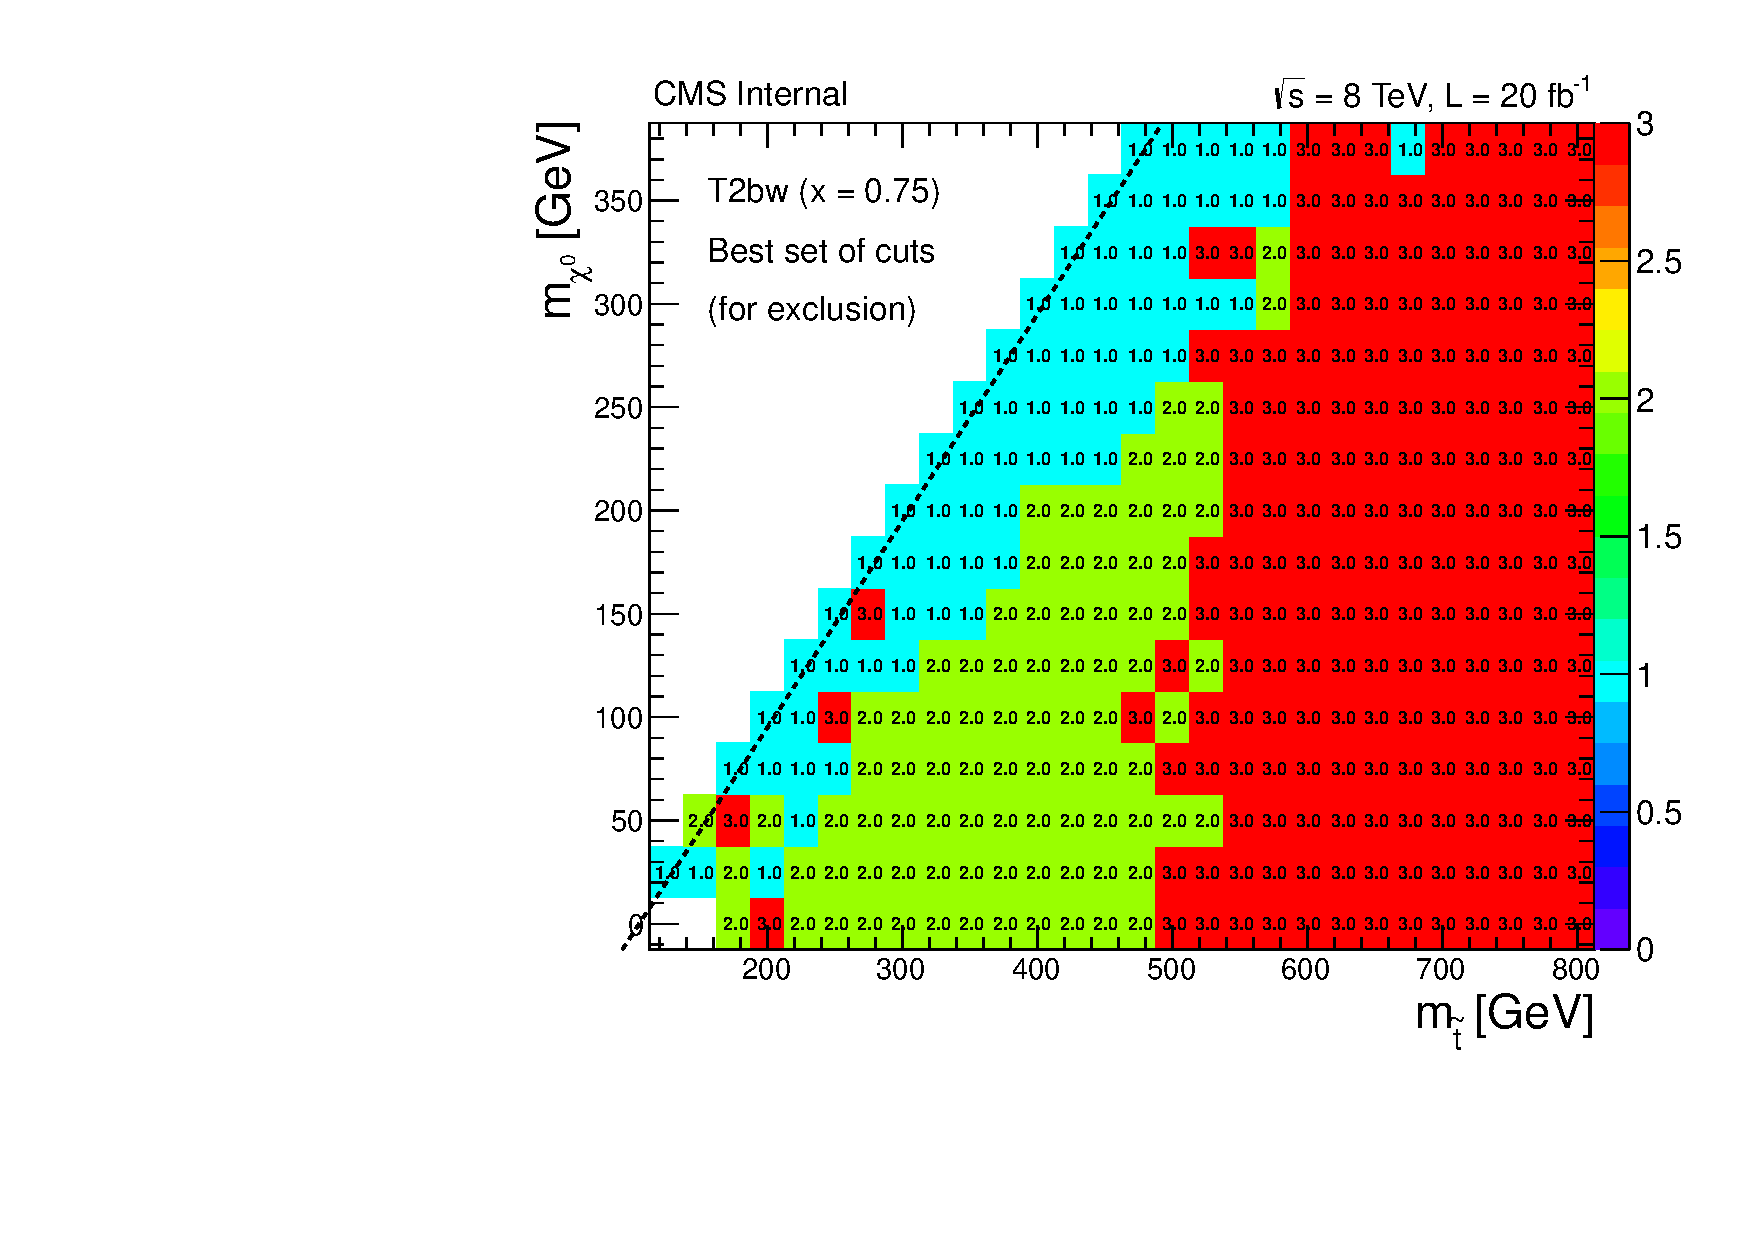
\includegraphics[width=0.37\textwidth]{cutAndCountPerformances/bestSet_T2bw075}
                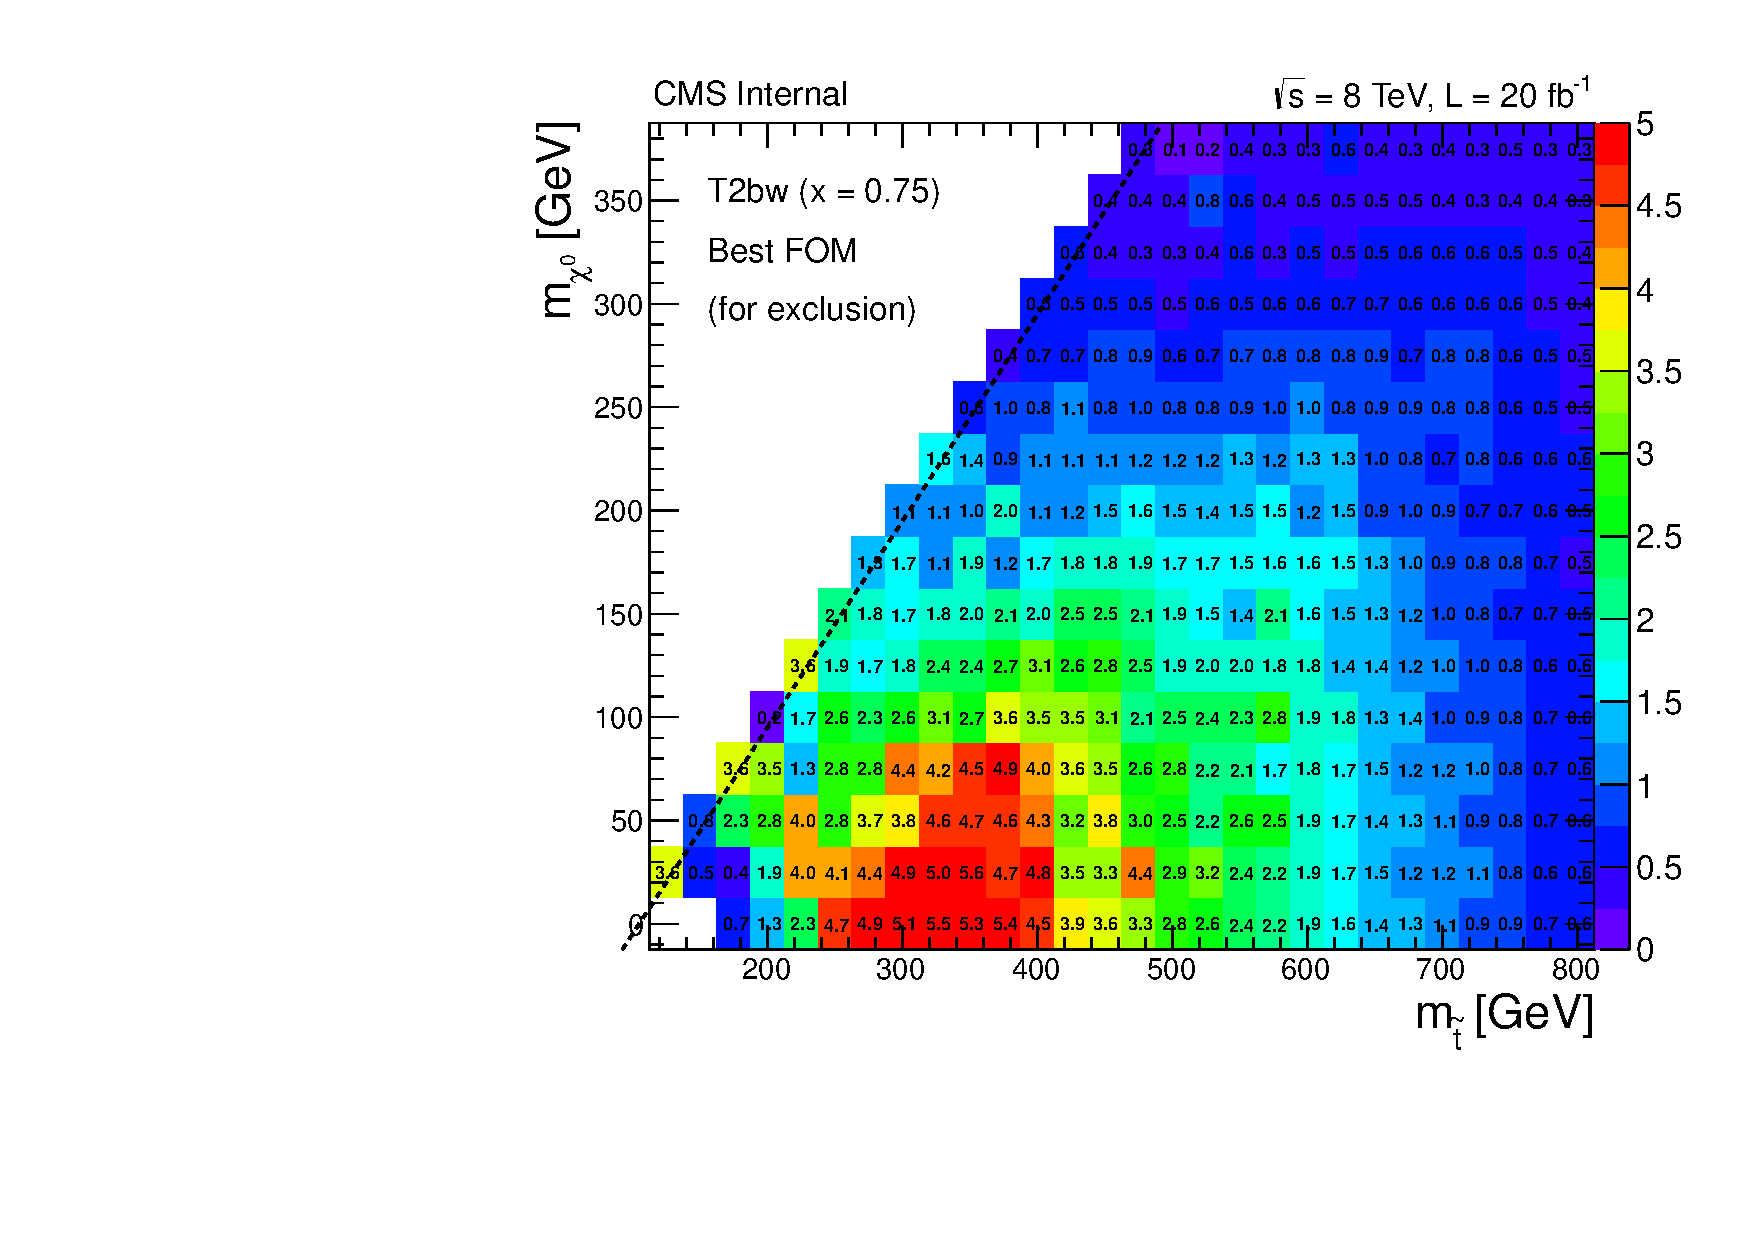
\includegraphics[width=0.37\textwidth]{cutAndCountPerformances/bestFOM_T2bw075}\\
                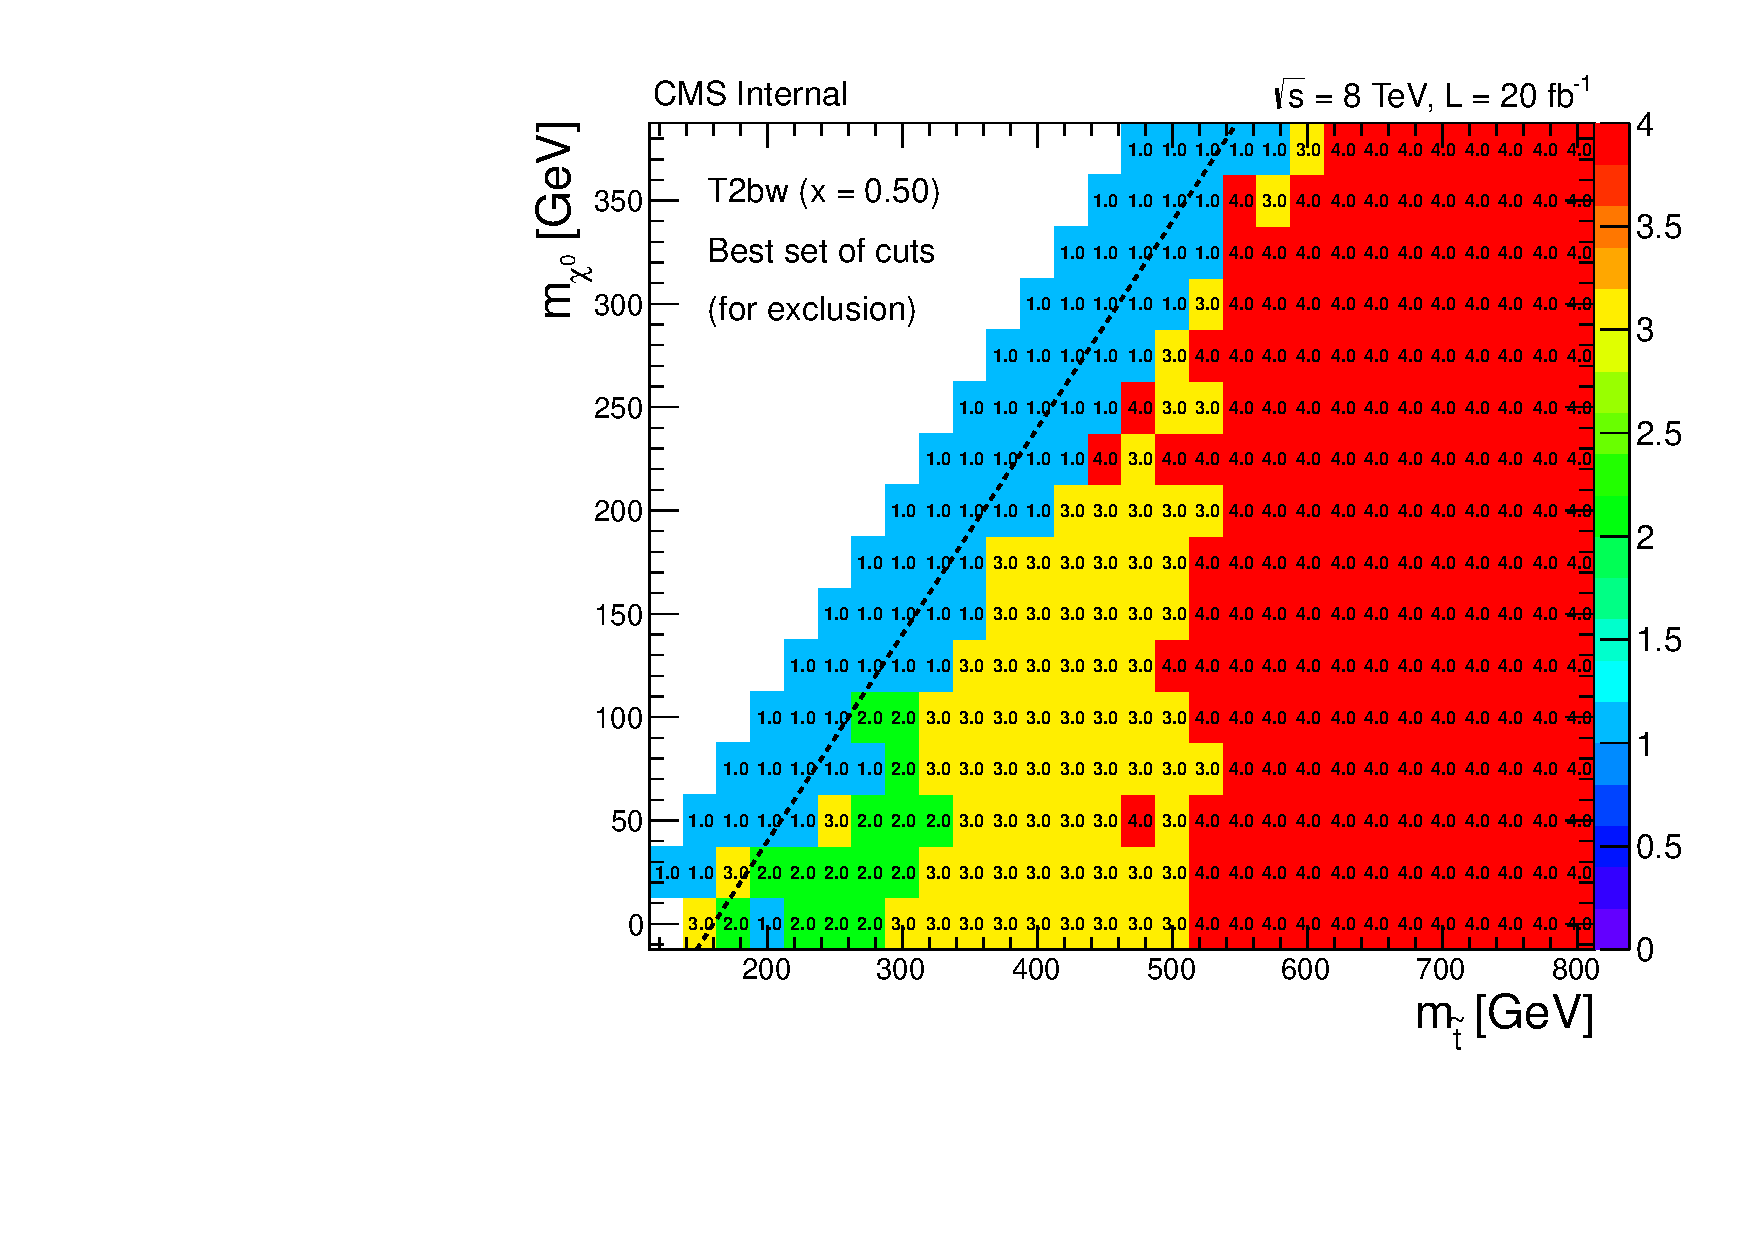
\includegraphics[width=0.37\textwidth]{cutAndCountPerformances/bestSet_T2bw050}
                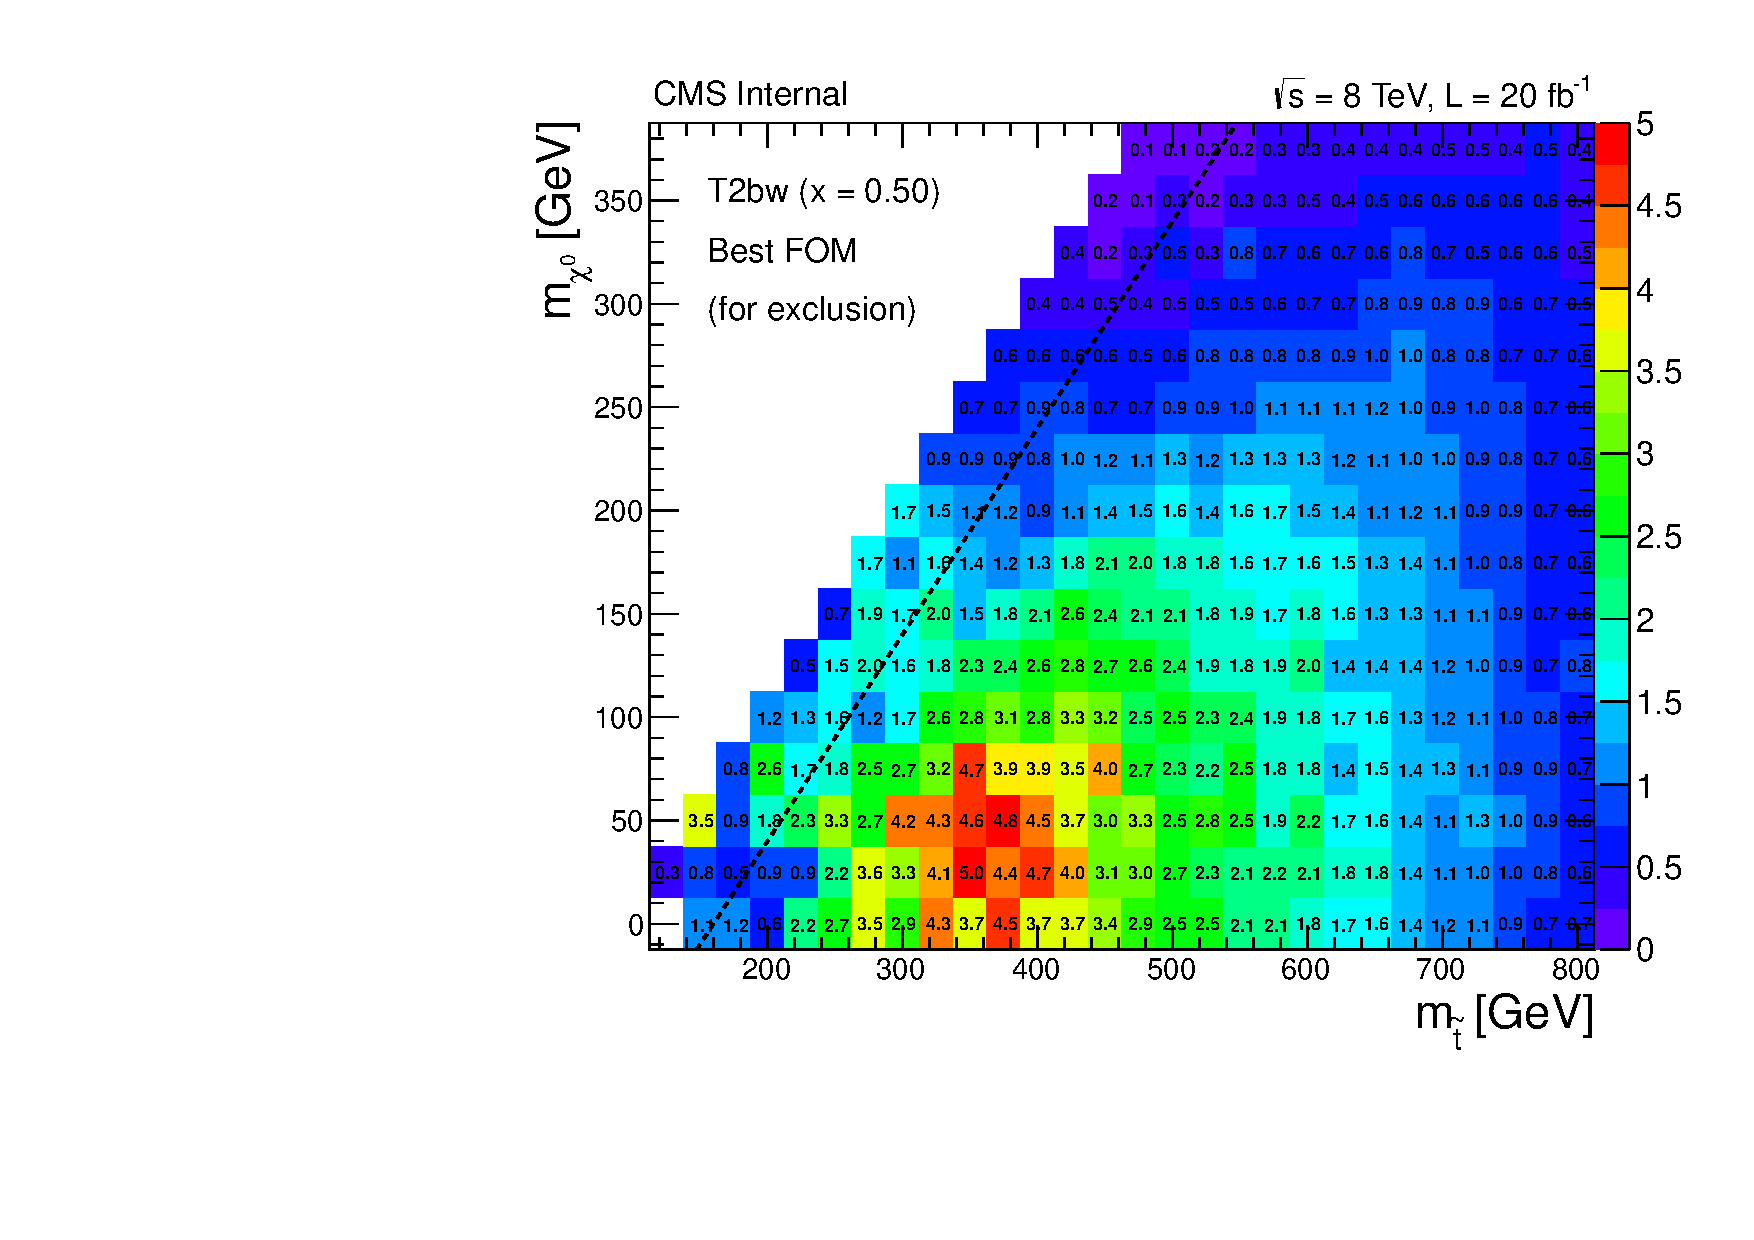
\includegraphics[width=0.37\textwidth]{cutAndCountPerformances/bestFOM_T2bw050}\\
                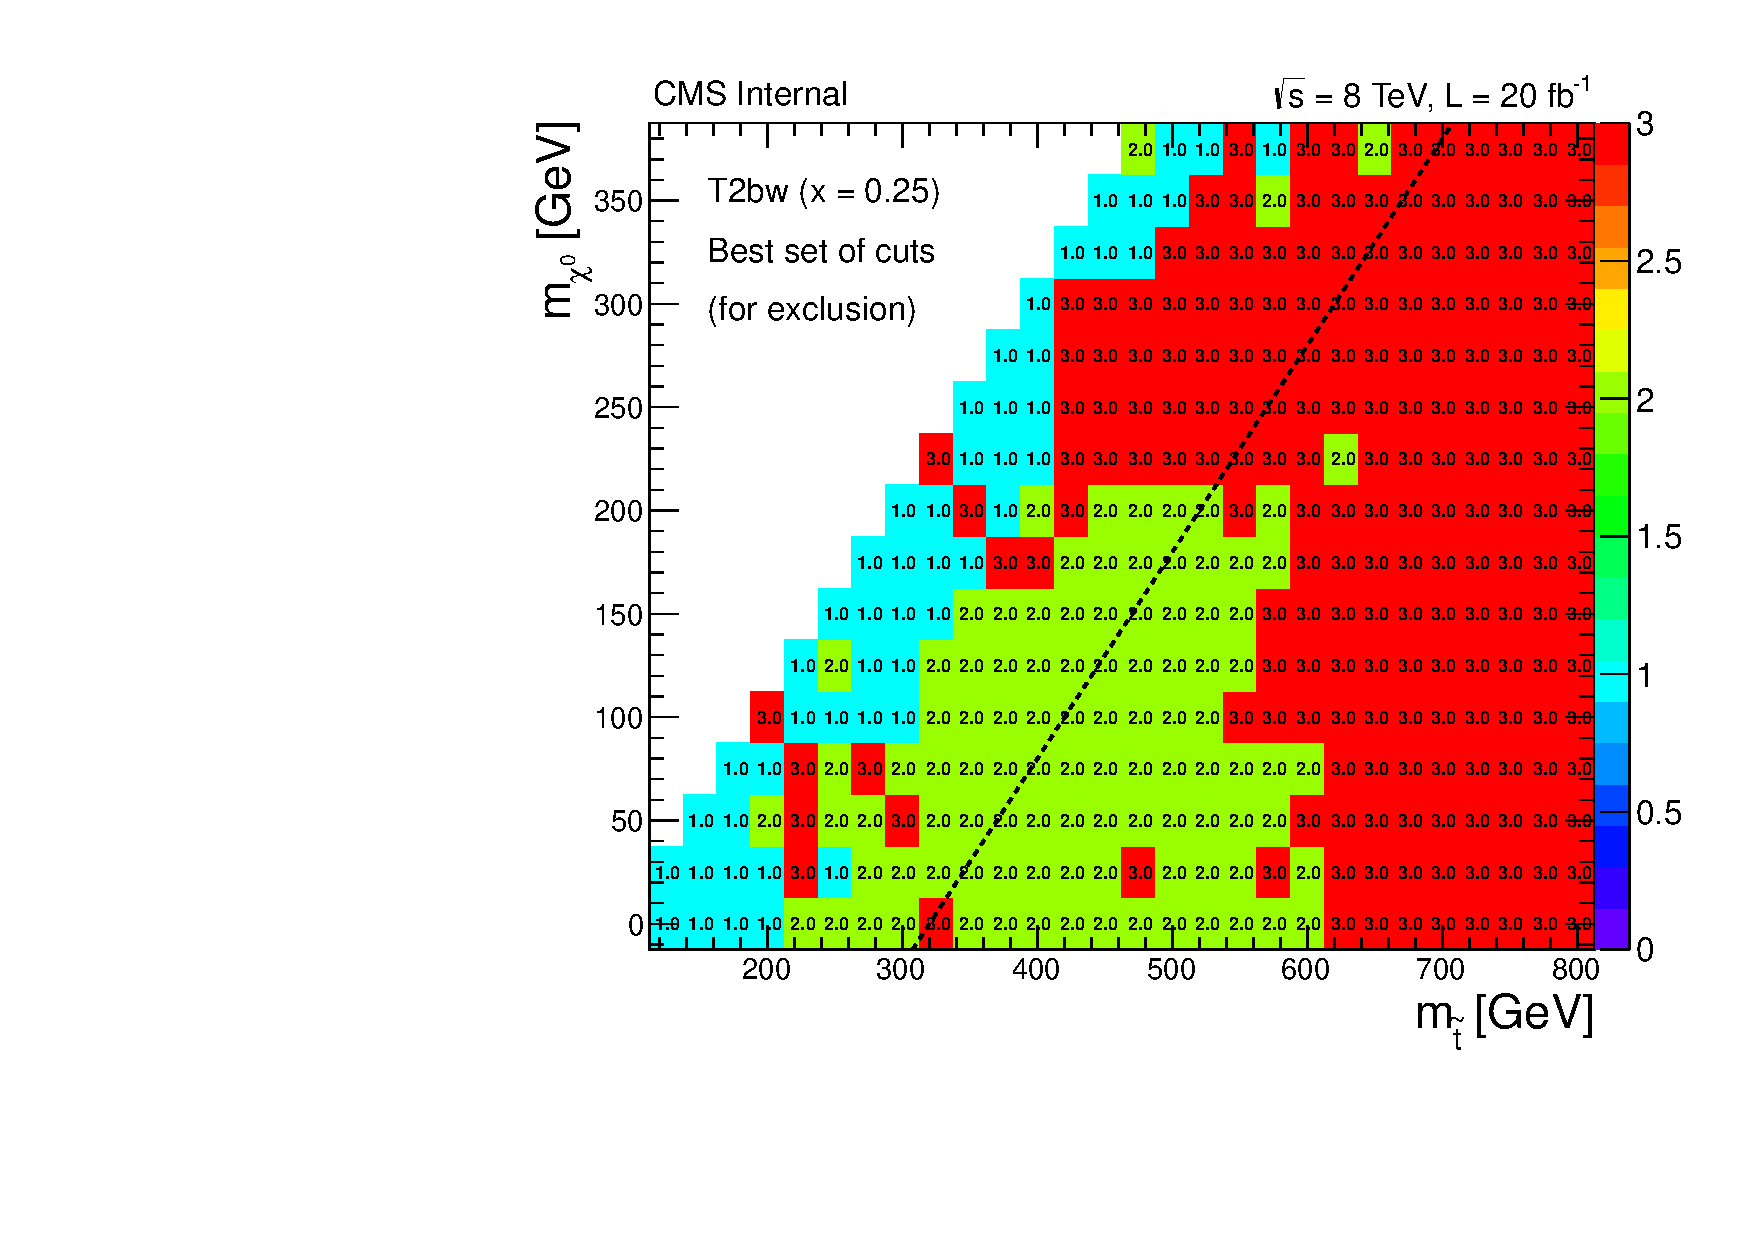
\includegraphics[width=0.37\textwidth]{cutAndCountPerformances/bestSet_T2bw025}
                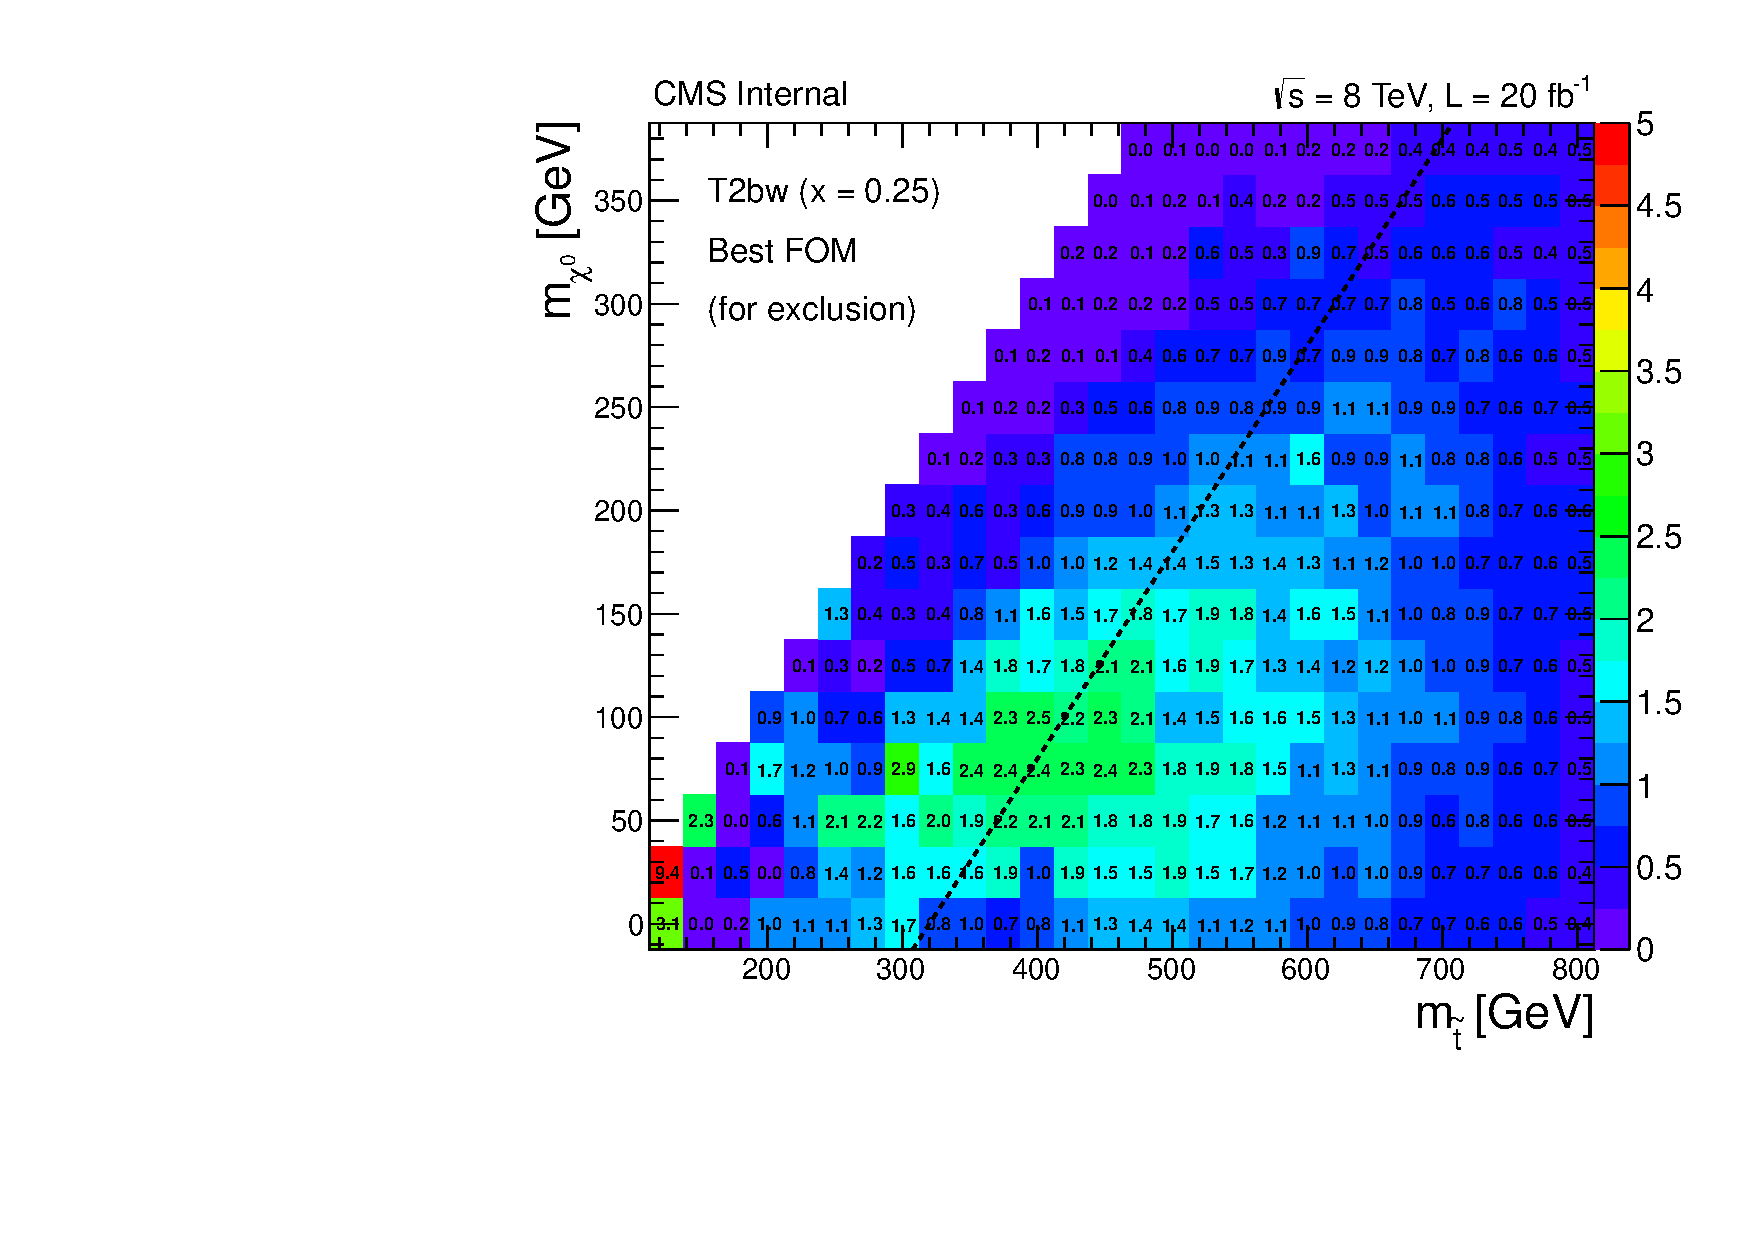
\includegraphics[width=0.37\textwidth]{cutAndCountPerformances/bestFOM_T2bw025}
                \caption{Best set of cuts (on the left) and performances in term of
                FoM$_\text{exclusion}$ (on the right) for the $\lstop \rightarrow t
                \lneutralino$ decay mode (first row) and $\lstop \rightarrow b \lchargino$
                decay mode with x = 0.75 (second row), 0.50 (third row) and 0.25 (last row).
                \todo{Maybe redo performance plot using the excluded signal strength formula+ contour at mu = 1, or if not show contour at FoM=2}}
                \label{fig:cutAndCountPerformances}
            \end{figure}

        \subsection{BDT-based signal regions}
        %==============================================================

        For the multivariate approach, several BDT are trained on slices of $\deltam$ in the $(\mass{\lstop},\mass{\lneutralino})$
        space against the $t\bar{t}$ background only. The choice of the variable is driven by an iterative method where variables
        are added to BDT and kept if the performances are overall significantly improved across different slices of $\deltam$. The
        performances of the BDTs are quantified by optimizing the cut on the BDT output with respect to a discovery-oriented
        FoM, considering all the backgrounds and assuming a relative systematic uncertainty of 15\%.

        The set of variables used are presented on Table \ref{tab:BDTVariableUsage} as function of the decay mode. The definition
        of the training region in the $(\mass{\lstop},\mass{\lneutralino})$ is then being looked at, noticing that some of the
        $\deltam$ slices can be merged together as the performances of the training are similar, essentially because the kinematic
        is not strongly different when moving from one slice to the other. The optimization of the cut on the BDT output is then
        performed by iteratively looking at the excluded cross-section after the full procedure explained in the following sections.
        The cuts are tuned manually to optimize the sensitivity accordingly. Here, because of the cross-section regimes leading to
        different amount of signal statistics, it is noticed that there is sometimes a significant gain in loosening or tightening
        the cut inside a same training region.

        The final definition of the training regions is presented on Figure \ref{fig:BDTTrainingRegions}. Each number represents a
        different BDT training. The dashed lines represent the cases when one training region leads to several cuts applied to define
        signal regions.

        \begin{table}[h!]
            \begin{center}
                \begin{tabular}{|c|cc|}

                    \hline
                    Variable                            & T2tt      & T2tt      \\
                                                        & off-shell & on-shell  \\
                    \hline
                    $\MET$                              & $\times$  & $\times$  \\
                    $H_{T}^\text{ratio}$                & $\times$  & $\times$  \\
                    $\pT(\text{lead. } \ell)$           & $\times$  & $\times$  \\
                    $\Delta\phi(j_{1,2},\vec{\MET})$    & $\times$  & $\times$  \\
                    $N_\text{jets}$                     & $\times$  & $\times$  \\
                    \hline
                    $\pT(\text{lead. jet})$             &           & $\times$  \\
                    $\Delta R( \ell, \text{lead. } b)$  &           & $\times$  \\
                    hadronic top $\chi^2$               &           & $\times$  \\
                    $M_{T2}^W$                          &           & $\times$  \\
                    $M_{\ell b}$                        & $\times$  &           \\
                    $\pT(\text{lead. } b)$              & $\times$  &           \\
                    \hline
                \end{tabular}
                \begin{tabular}{|c|ccc|}

                    \hline
                    Variable                            & T2bw      & T2bw      & T2bw      \\
                                                        & $x=0.25$  & $x=0.50$  & $x=0.75$  \\
                    \hline
                    $\MET$                              & $\times$  & $\times$  & $\times$  \\
                    $M_{T2}^W$                          & $\times$  & $\times$  & $\times$  \\
                    $M_{\ell b}$                        & $\times$  & $\times$  & $\times$  \\
                    $M_{3 b}$                           & $\times$  & $\times$  & $\times$  \\
                    $\pT(\text{lead. } \ell)$           & $\times$  & $\times$  & $\times$  \\
                    $\Delta\phi(j_{1,2},\vec{\MET})$    & $\times$  & $\times$  & $\times$  \\
                    $N_\text{jets}$                     & $\times$  & $\times$  & $\times$  \\
                    \hline
                    $\pT(\text{lead. } b)$              & $\times$  & $\times$  &           \\
                    $\Delta R( \ell, \text{lead. } b)$  &           & $\times$  &           \\
                    $H_{T}$                             &           &           & $\times$  \\
                    $\pT(\text{lead. jet})$             &           &           & $\times$  \\
                    \hline
                \end{tabular}
                \caption{List of variables considered for the training of the BDT
                as function of the decay mode. A $\times$ mark indicate that the variable
                is used in the final trainings.}
                \label{tab:BDTVariableUsage}
            \end{center}
        \end{table}

            \insertFourFigures{BDTTrainingRegions}
                              {BDT/training_T2tt}
                              {BDT/training_T2bw075}
                              {BDT/training_T2bw050}
                              {BDT/training_T2bw025}
                              {0.49}
                              {Slicing of the $(\mass{\lstop},\mass{\lneutralino})$ space
                              to define the training region of the BDTs. Some training
                              regions are subdivised into subregions where different cuts
                              are applied on the BDT output in order to adapt the sensitivity
                              to the local cross-section. \todo{Fix printability of plots}}

    \section{Background estimation \label{sec:analysis_backgroundEstimation}}
    %==============================================================

        \subsection{Overview}
        %==============================================================

    In this section, we focus on the estimation of the different background contributions.
    Four kinds of control regions are defined by inverting some of the requirements of the
    preselection and signal regions, as illustrated on Figure \ref{fig:backgroundEstimationOverview}.
    Each of these aim to provide signal-free sectors in which to check how good is the
    modeling of the backgrounds by the Monte-Carlo and perform data-driven estimations.

        \insertFigure{backgroundEstimationOverview}{0.7}
                     {Overview of the control regions used in the background estimation method. \todo{Fix printability of this sketch?}}

    The $\MT$-peak control region is defined by looking at events satisfying $50 < \MT <
    80\GeV$ instead of the signal region $\MT$ requirement. This control region is enriched
    in $\oneLeptonTop$ and is used as a well-controlled region in which to normalize the
    $\oneLeptonTop$, $\Wjets$ and $\diLeptonTop$ as documented in \ref{sec:MTpeakNormalization}.

    The $0\, b\text{-tag}$ control region is defined by requiring no $b$-tagged jet in the
    event. This region is enriched in $\Wjets$ and $\oneLeptonTop$ and is used to control
    and correct the tail of $\MT$ for these two components as described in \ref{sec:MTtailCorrection}.

    The $2\ell$ control region is defined by requiring exactly two selected leptons instead
    of one, at least one jet, and lowering the $\MET$ cut to $50 \GeV$. Additionnally, to limit the
    contribution from Drell-Yan, we veto events where the invariant mass of the dilepton
    system, $\mass{\ell\ell}$, is such that $\left|\mass{\ell\ell} - m_{Z}\right| < 15 \GeV$.
    Finally, the reversed veto control region is defined by requiring exactly one selected
    lepton and reversing the second lepton veto, effectively asking for an isolated track
    or $\tau$ as defined in \ref{sec:vetoLeptons}. This region  is intended to control
    the modeling of the second lepton veto. Both the $2\ell$ and reversed veto are being
    looked at on the whole $\MT$ range and are not used to derive scale factors but only
    systematic uncertainties on the background as detailed in \ref{sec:background_systematics}.

    Table \ref{tab:cutflowControlRegions} shows a breakdown of the background contributions
    in the different control regions at the preselection level.

\begin{table}[h!]
    \centering
\begin{tabular}{|c|cccc|}
    \hline
                     & $\MT$-peak       & $0\, b\text{-tag}$ ($M_T$ tail) & reversed veto    & 2 leptons             \\
    \hline
     $\oneLeptonTop$ & 18523 $\pm$ 55   &  1213 $\pm$ 14        &  7030 $\pm$ 34   &   41 $\pm$ 2.7  \\
     $\diLeptonTop$  &   656 $\pm$ 10   &   382 $\pm$ 8         &  7066 $\pm$ 34   & 9211 $\pm$ 39   \\
     $\Wjets$        &  1470 $\pm$ 24   &  2669 $\pm$ 33        &   331 $\pm$ 11   &  2.1 $\pm$ 0.9  \\
     rare            &  1209 $\pm$ 23   &   198 $\pm$ 7         &  1093 $\pm$ 20   &  626 $\pm$ 15   \\
    \hline
     total SM        & 21859 $\pm$ 66   &  4462 $\pm$ 38        & 15521 $\pm$ 53   & 9882 $\pm$ 42   \\
    \hline
\end{tabular}
    \caption{Breakdown of the yield of the different background categories in the four
    control regions without applying any signal region cuts. Uncertainties are statistical only.}
    \label{tab:cutflowControlRegions}
\end{table}

        \subsection{Background normalization in $\MT$-peak \label{sec:MTpeakNormalization}}
        %==============================================================

    The $\MT$-peak control region, defined as $50 < \MT < 80 \GeV$ is the first step of the
    background estimation method. It is used to normalize the $\oneLeptonTop$, $\Wjets$ and
    $\diLeptonTop$ components while the rare component is taken directly from Monte-Carlo.
    It is important to note that this normalization is done for each signal region individually,
    effectively allowing to absorb disagreements caused by cuts on not-so-well modeled
    variables and uncertainty on the jet energy scale, the trigger efficiency, the lepton
    identification efficiency and the luminosity.

    To separate the effect of the second lepton veto, the  normalization is done in two
    steps : first, a scale factor $\SFpre$ is computed before the application of the
    second lepton veto, substracting the rare component :

    \begin{equation}
        \SFpre \definedAs \left( \frac{N(\text{data}) - N(\text{rare})}{N(\oneLeptonTop) + N(\Wjets) + N(\diLeptonTop)} \right)
        \label{eq:SFpreDefinition}
    \end{equation}

    $\SFpre$ is used to normalize only the $\diLeptonTop$ component. Another scale factor,
    $\SFpost$ is used after application of the second lepton veto, substracting the rare
    and the corrected $\diLeptonTop$ component :

    \begin{equation}
        \SFpost \definedAs \left( \frac{N(\text{data}) - N(\text{rare}) - \SFpre \times N(\diLeptonTop)}{N(\oneLeptonTop) + N(\Wjets)} \right)
        \label{eq:SFpostDefinition}
    \end{equation}

     When applying no signal region cuts, $\SFpre$ and $\SFpost$ are equal to
     $(1.06 \pm 0.01)$ and $(1.05 \pm 0.01)$ respectively. This values, while not
     being compatible with 1, can be interpreted as a relatively small disagreement
     which is attributed to the misknowledge of the previously listed effects. Across the
     different cut-based signal regions, these scale factors range from $0.8$ to $1.4$,
     sometimes only compatible with unity at 3 standard deviations. The magnitude of this
     effect is attributed to bad modelization of the far tail of some variables in the
     Monte-Carlo.

        \subsection{$\MT$-tail correction in the $0\, b\text{-tag}$ region \label{sec:MTtailCorrection}}
        %==============================================================

    The $0\, b\text{-tag}$ control region allows to control the tail of $\MT$ for the $\Wjets$ and
    $\oneLeptonTop$ components. Before looking at the tail, however, we start by normalizing
    the background in the $\MT$ peak of this control region, in a similar fashion to what
    is done in \ref{sec:MTpeakNormalization}. This is done by introducing $\SFnobtag$,
    used to normalize the $\Wjets$ and $\oneLeptonTop$ contributions :

    \begin{equation}
        \SFnobtag \definedAs \left( \frac{N(\text{data}) - N(\text{rare}) - N(\diLeptonTop)}{N(\oneLeptonTop) + N(\Wjets)} \right)
        \label{eq:SF0btagDefinition}
    \end{equation}

    Without applying any signal cuts, $\SFnobtag$ is found to be $(0.99 \pm 0.01)$.
    After normalization to the peak, a clear disagreement in the tail of $\MT$ is observed
    for $\MT > 100 \GeV$ between the data and Monte-Carlo, as shown on Figure
    \ref{fig:templateFit/MT_notCorrected}. This is an important point of the analysis as
    it means that the Monte-Carlo needs to be corrected to have a reliable prediction of
    the $\oneLeptonTop$ and $\Wjets$ in the $\MT$ tail. \todo{Is it really a 'known'
    disagreement ... ? SMP-14-020, AN-2014/279 and AN-2014/114  see a disagreement
    for Wjets, but B2G-14-004 doesn't see anything for ttbar...}\todo{MTW sensitivity
    to MET also discussed in AN-15-013}.

    \insertFigure{templateFit/MT_notCorrected}{0.55}
                 {Data/MC comparison on the full $M_T$ distribution in the $0\, b\text{-tag}$ control
                 region at preselection level, after propagation of $\SFnobtag$. A clear
                 discrepancy is visible for $\MT > 100 \GeV$.}

    One can investigate the cause of the disagreement by first getting a better idea from
    the Monte-Carlo simulation of what is causing $\oneLeptonTop$ and $\Wjets$ events
    to each the tail of $\MT$. The resolution of $\MT$ is strongly related to both the
    resolution in $\pT$ of $\vec{\MET}$ and $\Delta\phi$ with the lepton. The relative
    resolution of $\MET$ and $\Delta \phi$ is investigated, defined as the ratio of the
    reconstructed quantity versus the generated quantity using only the generated
    neutrinos from the $W$ in the event. \todo{Maybe fix misleading 'resolution' name as here gen MET
    is only gen neutrino-MET...}. Figure \ref{fig:MTtailResolution} shows the distribution of the relative
    resolution of $\MET$ and $\Delta \phi$ as function of $\MT$ for the $\oneLeptonTop$
    background and its mean for each background.

    \insertFourFigures{MTtailResolution}
                      {MTtailResolution/MTvsMETReso}
                      {MTtailResolution/MTvsDeltaPhiReso}
                      {MTtailResolution/MTvsMeanMETReso}
                      {MTtailResolution/MTvsMeanDeltaPhiReso}
                      {0.45}
                      {$\MET$ and $\Delta \phi$ relative resolution as function of $\MT$,
                      using the generated $MET$ from neutrinos coming from a $W$, on top
                      showing the full 2 dimensional distribution and on bottom showing
                      the evolution of the mean resolution for each background. Error
                      bars corresponds to the uncertainties on the mean.}

    The results of this small investigation tends to point out that the $\MT$ tail for
    the $\oneLeptonTop$, $\Wjets$ and rare backgrounds originates more from the
    misreconstruction of the magnitude of the $\MET$ rather than it's direction. Small
    features are however observed in the $\Delta \phi$ spectra which can originate from
    other sources of $\MET$ in the event such as neutrinos inside $b$-jets.
    \todo{Complete this part later with results from Master students ?}

    %So far, the understanding of this disagreement comes from two source : first, the
    %off-shell contributions of $\Wjets$ is underestimated by the simulation, and second,
    %detector effects leads to a larger tail for the $\oneLeptonTop$ events.
    So far, the method used to correct the discrepancy is to compute ad-hoc scale factors
    using a template fit that estimate separately the contribution of $\oneLeptonTop$ and
    $\Wjets$ from the data. To do this, we use $\MlbPrime$ which was found to have a good
    discriminating power between the two process categories and being well discribed in
    the peak of $\MT$, as shown on Figure \ref{fig:MlbPrimeForTemplateFit}.

        \insertFourFigures{MlbPrimeForTemplateFit}
                          {templateFit/Mlb_0b_peak}
                          {templateFit/Mlb_0b_tail}
                          {templateFit/preselection_Mlb_noFit}
                          {templateFit/preselection_Mlb_withFit}
                          {0.45}
                          {Distribution of $\MlbPrime$ in the $0\, b\text{-tag}$ control region, data/MC comparison in the $M_T$ peak (top left), superimposed and normalized $\oneLeptonTop$ and $\Wjets$ components in the $M_T$ tail (top right), data/MC comparison in the $M_T$ tail before correction of the Monte-Carlo (bottom left) and after correction (bottom right). On the bottom right, the uncertainty of the scale factors are propagated in the ratio.}

    The method is implemented using the \textsc{RooFit} toolbox \refNeeded with the Minuit2
    implementation of the \textsc{Migrad} minimizer algorithm \refNeeded. The normalization
    of the $\oneLeptonTop$ and $\Wjets$ components are free parameters translated in term
    of scale factors, $SF_{\oneLeptonTop}$ and $SF_{\Wjets}$, while the normalization of
    the $\diLeptonTop$ and rare components are taken from the Monte-Carlo and constrained
    with a 20\% uncertainty during the fit process. To validate the method, a closure test
    is performed by generating toy data from the Monte-Carlo where arbitrary scale factors
    where injected. The estimated scale factors are then compared to the input scale factors.
    A very good linearity is found for scale factors varying from 0.10 to 3. The fit is
    performed both in the $\MT$ peak and tail regions and we extract $SFR = SF^{\text{tail}}
    / SF^{\text{peak}}$ for both processes, representing the discrepancy in the tail
    independently from the peak normalization. Different sources of systematic uncertainty
    are considered : the jet energy scale, the normalization of the rare background, the
    Monte-Carlo statistics, the choice of the minimizer algorithm, the choice of the
    initial fit conditions, the generator setup for $t\bar{t}$ (using \textsc{Powheg} or
    \textsc{MadGraph}, varying the matching parameters, RGE scale, top mass, applying or
    not the top $\pT$ reweighting). The most important sources are the Monte-Carlo statistics
    (leading to 11\% of relative uncertainty on SFR), the generator scale (9\%) and the jet
    energy scale. A conservative 20\% is used as relative systematic uncertainty.

    Without applying any signal region cuts, $\SFRoneLeptonTop$ and $\SFRWjets$ are found
    to be $(1.04 \pm 0.16 (\text{stat.}) \pm 0.21 (\text{syst.}))$ and $(1.33 \pm 0.10
    (\text{stat.}) \pm 0.27 (\text{syst.}) )$ respectively. The plot on Figure \ref{fig:MlbPrimeForTemplateFit}
    illustrate the impact on the $\MlbPrime$ data/MC comparison after propagating the scale
    factors. For the cut-based signal regions, we use the scale factors derived from a
    single $M_T$ cut associated to the signal region as shown on Figure \ref{fig:templateFit/CnC_MTcuts}.
    To cover possible correlation between the $SFR$ and $\MET$, the uncertainty from the
    single $\MET$ or $\MET/\sqrt{H_T}$ cut associated to the signal region is also
    quadratically added to the scale factor. These scale factors are shown on Figure \ref{fig:templateFitCnCResultsMET}.

    For the BDT signal regions, to be as close as possible to the kinematic of the BDT tails,
    we choose cuts on each BDT outputs such as at least 25\% of the background is still
    selected and apply the template fit method in that region. Two common scale factors
    to be applied to each BDT are then computed by averaging across all the trainings.
    The values found are $\SFRoneLeptonTop = (1.38 \pm 0.61)$ and $\SFRWjets = (1.21 \pm 0.36)$.

        \insertFigure{templateFit/CnC_MTcuts}
                     {0.6}
                     {Template fit results for individual cuts on $\MT$ after
                     preselection. The uncertainties shown are statistical only.}

        \insertTwoFigures{templateFitCnCResultsMET}
                         {templateFit/CnC_METcuts}
                         {templateFit/CnC_METoverSqrtHTcuts}
                         {0.45}
                         {Template fit results for invidiviual cuts on $\MET$ (left)
                         and $\MET/\sqrt{H_T}$ (right) after preselection + $\MT > 100\GeV$.
                         The uncertainties shown are statistical only.}

        \subsection{Control of $\diLeptonTop$ component and second lepton veto \label{sec:analysis_controlDileptonTop}}
        %==============================================================

        The 2-lepton and reversed veto control regions allow to check for the good modeling
        of the $\diLeptonTop$ background and the veto lepton definition. For the
        2 lepton control region, $\MT$ is defined using the leading lepton and ignoring
        the second one. The $\MT$-peak of the reversed veto control region is dominated by
        $\oneLeptonTop$ where a fake second lepton was reconstructed while the $\MT$-tail
        is dominated by $\diLeptonTop$ with a true second lepton. As for the $\MT$-peak
        normalization, we introduce scale factors to normalize the backgrounds in the peak
        of $\MT$ and quantify the agreement in the tail.

        In the reversed veto region, we define $\SFveto$ in a similar fashion as $\SFpost$,
        to control the fake-dominated region, and $\SFvetoTail$ to control the true second
        lepton dominated region after propagation of all the relevant scale factors including
        $\SFRoneLeptonTop$.

        Without applying any signal region cuts, we find $\SFveto = (1.18 \pm 0.03)$ and
        $\SFvetoTail = (1.07 \pm 0.02)$. The relatively large value of $\SFveto$ is
        interpreted as a mismodeling of the fake rate of the veto lepton by the Monte-Carlo
        and, despite being not compatible with unity, is not used to compute the prediction
        in the signal region because its effect is already included in $\SFpost$. The
        value of $\SFvetoTail$ also manifest a discrepancy in the veto lepton selection
        efficiency. Despite the fact that this scale factor is not propagated to the
        signal region, a systematic is later introduced to cover this effect.

        In the 2 leptons control region, we define $\SFtwoLep$ and $\SFtwoLepTail$ to
        control respectivelly the whole $\MT$ distribution and the tail of it.
        Without applying any signal region cuts, we find $\SFtwoLep = (0.96 \pm 0.01)$
        and $\SFtwoLepTail = (1.01 \pm 0.02)$ showing therefore a good modeling of $\MT$
        for this background.

        Another important check in the 2 leptons control region is the jet multiplicity
        modeling of $\diLeptonTop$ as the four jets requirements corresponds to two
        additional jets coming from radiations or pile-up for this background.
        Figure \ref{fig:} presents the distribution of the number of selected jets after
        application of $\MT>100$, which is found in good agreement.

        Figure \ref{fig:preselMT2leptonAndLepPlusVeto} presents the full $\MT$
        distributions for the reversed veto and two leptons control region.

        \begin{figure}[h!]
            \centering
            \includegraphics[width=0.45\textwidth]{controlPlots/reversedVeto_noMTCut/MT}
            \includegraphics[width=0.45\textwidth]{controlPlots/2leptons_noMTCut/MT}
            \caption{Full $\MT$ distributions for the reversed veto control region (on the left) and two leptons control region (on the right). On the left, $\SFpre$, $\SFveto$, $\SFRoneLeptonTop$ and $\SFRWjets$ are propagated. On the right, no scale factors is applied.}
                    \label{fig:preselMT2leptonAndLepPlusVeto}
        \end{figure}

        \insertFigure{controlPlots/2leptons/nJets}
                     {0.5}
                     {Distribution of the number of selected jets in the two leptons control region after applying $\MT > 100$.}

        \subsection{Control plots at preselection level}
        %==============================================================

        Figure \ref{fig:preselControlPlots} shows control plots for $\MT$, $\MET$ and $M_{T2}^W$ in the different control regions at the preselection level. \todo{Add comments here but I don't know what to say :/}

            \begin{figure}[h!]
                \centering
                \includegraphics[width=0.325\textwidth]{controlPlots/MTpeak/MT}
                \includegraphics[width=0.325\textwidth]{controlPlots/MTpeak/MET}
                \includegraphics[width=0.325\textwidth]{controlPlots/MTpeak/MT2W}\\
                \includegraphics[width=0.325\textwidth]{controlPlots/0btag/MT}
                \includegraphics[width=0.325\textwidth]{controlPlots/0btag/MET}
                \includegraphics[width=0.325\textwidth]{controlPlots/0btag/MT2W}\\
                \includegraphics[width=0.325\textwidth]{controlPlots/reversedVeto_noMTCut/MT}
                \includegraphics[width=0.325\textwidth]{controlPlots/reversedVeto_noMTCut/MET}
                \includegraphics[width=0.325\textwidth]{controlPlots/reversedVeto_noMTCut/MT2W}\\
                \includegraphics[width=0.325\textwidth]{controlPlots/2leptons_noMTCut/MT}
                \includegraphics[width=0.325\textwidth]{controlPlots/2leptons_noMTCut/MET}
                \includegraphics[width=0.325\textwidth]{controlPlots/2leptons_noMTCut/MT2W}\\
                \caption{A few control plots, showing the data/MC comparison for $\MT$ (left column),
                        $\MET$ (middle column) and $M_{T2}^W$ (right column) in the different control
                        regions : $\MT$-peak (first row), $0\, b\text{-tag}$ (second row), reversed veto (third
                        row) and 2 leptons (fourth row). The $\MT$-peak normalization and $\MT$-tail
                        correction scale factors are propagated where relevant.}
                        \label{fig:preselControlPlots}
            \end{figure}

        \subsection{Background prediction}
        %==============================================================

        The background prediction is obtained by taking the Monte-Carlo yield in the
        $\MT$-tail and propagating $\SFpre$ to the $\diLeptonTop$ component and $\SFpost$
        to the $\oneLeptonTop$ and $\Wjets$ component. The $\oneLeptonTop$ and $\Wjets$
        are also corrected with $\SFRoneLeptonTop$ and $\SFRWjets$ respectively. The
        prediction for the rare component is directly the Monte-Carlo yield in $\MT$-tail.
        The formula \ref{eq:prediction1ltop} to \ref{eq:predictionrare} below summarize
        the computation of the prediction. The procedure is repeated for each signal
        region as all the scale factors involved are signal-region dependent. As an
        illustration, Table \ref{tab:predictionPreselection} shows the comparison between
        the raw Monte-Carlo and the prediction obtained at preselection level.

        \begin{eqnarray}
            N^\text{pred}_\text{tail}(\oneLeptonTop) & = & N^\text{MC}_\text{tail}(\oneLeptonTop)  \times \SFpost \times \SFRoneLeptonTop \label{eq:prediction1ltop}  \\
            N^\text{pred}_\text{tail}(\Wjets)        & = & N^\text{MC}_\text{tail}(\Wjets)         \times \SFpost  \times \SFRWjets                             \\
            N^\text{pred}_\text{tail}(\diLeptonTop)  & = & N^\text{MC}_\text{tail}(\diLeptonTop)   \times \SFpre                                                \\
            N^\text{pred}_\text{tail}(\text{rare})   & = & N^\text{MC}_\text{tail}(\text{rare})                                           \label{eq:predictionrare}
        \end{eqnarray}

        \begin{table}[!h]
            \begin{center}
                \begin{tabular}{|l|c|c|}
                    \hline
                                             &  \textbf{Raw MC}    & \textbf{Prediction}       \\
                    \hline
                    \textbf{$\oneLeptonTop$} &  5970 $\pm$ 31      & 6526 $\pm$ 1632     \\
                    \textbf{$\diLeptonTop$}  &  2117 $\pm$ 18      & 2253 $\pm$  229     \\
                    \textbf{$\Wjets$}        &   477 $\pm$ 13      &  669 $\pm$  364     \\
                    \textbf{rare}            &   490 $\pm$ 13      &  490 $\pm$  245     \\
                    \hline
                    \textbf{Total SM}        &  9055 $\pm$ 41      & 9940 $\pm$ 1666     \\
                    \hline
                \end{tabular}
                \caption{ Background prediction at the preselection + $\MT > 100\GeV$ level.}
                \label{tab:predictionPreselection}
            \end{center}
        \end{table}

    \section{Systematic uncertainties \label{sec:analysis_systematics}}
    %==============================================================

        This section describes the sources of systematics uncertainties that are considered for the background and the signal.

        \subsection{Systematic uncertainties on the background \label{sec:background_systematics}}
        %==============================================================

            Several sources of systematic uncertainties are considered for the background,
            the most important ones being from the $\MT$-peak normalization, the $\MT$-tail
            correction and the $\diLeptonTop$ modeling of the $\MT$ tail.

            \subsubsection{Modeling of $\diLeptonTop$ in $\MT$ tail}

            As discussed in section \ref{sec:analysis_controlDileptonTop}, the modeling by
            the Monte-Carlo of the $\MT$ tail of the $\diLeptonTop$ background is found
            to be good in the 2 leptons and reversed veto control regions. As it is a
            major background of the analysis, a systematic uncertainty is nevertheless
            asserted to quantify the trust in the Monte-Carlo on a per-signal-region basis.

            To do this, one wants to probe the 2 leptons and reversed veto control regions
            as close as possible of the signal region. However, as the signal region cuts
            are sometimes quite tight, the remaining statistics in these control region is
            too low and doesn't allow a reasonnable check of the distributions. To work
            around this problem while still probing the tail of $\MT$ near the signal
            region, we define loosened cuts to check these scale factors with more
            statistics. These cuts are designed by requiring to have at least 30 events
            remaining in the tail of $\MT$ for the 2 lepton control region.

            For each of the relaxed control region, we compute the value of $\SFtwoLepTail$
            and $\SFvetoTail$ to quantify the agreement between data and the simulation in
            the tail of $\MT$. An enveloppe is then computed computed for each signal
            region to account for the spread of the scale factors for each of the
            associated control regions. For the cut-based signal regions, this lead to a
            relative uncertainty on the total yield varying from 1.5 to 35\%. For the
            BDT signal regions, this relative uncertainty is between 7 and 40\%.

            \subsubsection{Second lepton veto efficiency}
            %============================================

            The uncertainty on the efficiency of the second lepton veto is propagated to the
            fraction of $\diLeptonTop$ events that have a second lepton in the acceptance. For
            the isolated track veto lepton, this is defined as having a second generated
            $e/\mu$ or a one prong $\tau \rightarrow h$ with $\pT > 5 \text{ or } 10 \GeV$,
            respectively, with $\abseta < 2.4$. This fraction is between 50-70\% for all
            signal regions. The uncertainty for these events is 6\% and is obtained from
            tag-and-probe studies \refNeeded. Regarding the $\tau$ veto leptons, the
            events considered are those with a hadronic $\tau$ in the acceptance, with
            true visible transverse energy $> 20\GeV$ in $\abseta < 2.4$. This fraction is
            about $10 \sim 20 \%$ of the total. The uncertainty on the efficiency of the
            $\tau$-ID algorithm is 7\%, taken from $\tau$ group studies \refNeeded.

            \subsubsection{Uncertainty on $\SFRoneLeptonTop$ and $\SFRWjets$}
            %================================================================

            As described in section \label{sec:MTtailCorrection}, the $\MT$-tail correction
            scale factors for $\oneLeptonTop$ and $\Wjets$ are computed with an uncertainty
            coming from statistics in the $0\, b\text{-tag}$ control region and systematic effects
            from the template fit method itself, as well as . This uncertainty is propagated
            to the total background yield uncertainty and is one of the major contribution
            for the signal region with a large remaining fraction of $\oneLeptonTop$.
            For the cut-based signal regions, this corresponds to a relative uncertainty
            on the total background ranging from 0 to 15\% and up to 17\% for the BDT
            signal regions.

            \subsubsection{Statistic uncertainty in $\MT$ peak}
            %==============================================================

            The $\MT$-peak normalization scale factors are an important part of the background
            estimation procedure, but is nevertheless limited by the statistics available
            in the peak region. Therefore, the $\SFpre$ and $\SFpost$ scale factors come
            associated to an uncertainty, dominated by the event count of data. This
            uncertainty is propagated to the prediction in the tail. This lead to a
            relative uncertainty on the total background ranging from 2 to 15\% for the cut-based
            signal regions and between 3 and 40\% for the BDT signal regions.

            \subsubsection{Other sources of systematic uncertainties}
            %========================================================

            Other sources of uncertainties are taken into account though being small compared
            to the ones described in the previous subsections :
            \begin{itemize}
                \item To cover the modeling of of ISR and FSR jets, the $N_\text{jets}$
                      distribution is studied in the 2 leptons control region. An
                      uncertainty of 2\% is asserted on the $\diLeptonTop$ background
                      from this check.
                \item To account for possible mismodeling of the relative proportions of
                      the backgrounds, the $\oneLeptonTop$ component cross-section
                      is varied by 10\% while the $\Wjets$ cross-section is varied by 50\%
                      during the background estimation procedure.
                \item As the rare category is quite difficult to estimate because composed
                      of a large number of background, its contribution is taken directly
                      from MC. We however put a conservative 50\% uncertainty in the
                      rate of this category.
                \item The Monte-Carlo statistics available in the $\MT$ tail being limited,
                      it also contributes to the systematic uncertainty on the final prediction.
            \end{itemize}

            \subsubsection{Summary of background uncertainties at preselection}
            %==============================================================

            Table \ref{tab:systematicSummary} shows a breakdown of the different systematics
            uncertainties that are considered, at preselection level and the range of them
            for the two kinds of signal regions. The relative importance of the individual
            systematics varies depending on the signal regions as the composition of the
            background itself varies : at preselection level, the importance of the
            $\SFRoneLeptonTop$ uncertainty is high as the $\oneLeptonTop$ component is still large.
            However for some signal regions, the $\diLeptonTop$ is the dominant contributions and
            uncertainty from the $\MT$-tail modeling is the leading systematic source.

            % Add range of uncertainties in the signal regions

            \begin{table}[!ht]
                \begin{center}
                    \begin{tabular}{|l|c|cc|}
                        \hline
                                                                       & Preselection    & Cut-based      & BDT             \\
                                                                       & + $\MT>100\GeV$ & signal regions & signal regions  \\
                        \hline
                        \textbf{$\diLeptonTop$ ($\MT$-tail modeling)}  & 1.6                      & 2-35         & 7-40    \\
                        \textbf{$\diLeptonTop$ (jets modeling)}        & 1.1                      & 1-4          & 0.5-4   \\
                        \textbf{$\diLeptonTop$ (2nd lepton veto)}      & 1.2                      & 0-4          & 1-4     \\
                        \textbf{$\SFRWjets$ uncertainty}               & 1.4                      & 0-6          & 0-5     \\
                        \textbf{$\SFRoneLeptonTop$ uncertainty}        & 16.4                     & 0-15         & 0-17    \\
                        \textbf{$\MT$-peak SF uncertainties}           & 0.7                      & 2-15         & 3-40    \\
                        \textbf{Cross-sections and MC stat}            & 1.9                      & 7-48         & 7-47    \\
                        \hline
                        \textbf{total}                                 & 16.8                     & 12-50        & 25-60   \\
                        \hline
                    \end{tabular}
                    \caption{Summary of the relative uncertainties at preselection+$\MT>100\GeV$
                    and range of relative uncertainties with respect to the total predicted
                    background yield for cut-based signal regions and BDT signal regions.
                    \label{tab:systematicsSummary}}
                \end{center}
            \end{table}

        \subsection{Systematic uncertainties on the signal}
            %==============================================================

        While the background prediction is dominated by data-driven systematic
        uncertainties, the signal uncertainty sources are more related to the
        confidence in the different element of the construction of the Monte-Carlo
        samples and algorithm used.

        The limited available statistics of the signal sample leads to a 2\% maximal
        2\% uncertainty. The integrated luminosity is known with a precision of 2.2\%
        and is propagated to the uncertainty of the yield. The trigger efficiency
        used in the very first steps of the selection is known with a precision of 3\%.
        The lepton identification and isolation efficiency are observed to be consistent
        between data and Monte-Carlo within an envelope of 5\%.

        The jet energy scale uncertainty is studied by varying the jet energy corrections
        within their $\pm$1 sigma uncertainty before the jet selection. The variation is
        properly propagated into the $\MET$ value. During the process, we also assume a
        10\% uncertainty on the unclustered energy defined as $(\vec{\MET} + \sum_\text{jets}
        \vec{p} + \sum_\text{leptons} \vec{p})$ where jets and leptons are selected with looser
        $\pT$ and $\abseta$ requirements. This effect leads to a maximum 10\% uncertainty on
        the signal yields.

        The uncertainty on the reshaping of the $b$-tagging discriminator is also considered
        by varying the technique within $\pm$1 sigma uncertainy before the application of
        $b$-tagging requirements. This leads to a 3\% uncertainty on the signal yields.

        The uncertainty on the ISR jets reweighting applied on signal is taken from data/MC
        scale factors derived from the analysis of events with high $\diLeptonTop$ purity. The
        scale factors, function of the $\pT$ recoil of the system, are varied within their
        uncertainties and lead to a maximum variation of 8 and 10\% on the signal yield, depending
        of the decay mode.

        Finally, the uncertainty on PDF are calculated, following the PDF4LHC prescription,
        using the CT10, NNPDF 2.1, and MSTW2009 PDF sets. \refNeeded The impact on the
        signal efficiency range from 10 to 30\% depending on the signal mass point.

    \section{Signal contamination handling}
    %==============================================================

        Signal contamination occurs when a significant fraction of signal events is present in
        the control regons. While it doesn't affect the predicted yield for the background-only hypothesis
        ($H_0$), a significant contamination can bias the data-driven aspects of the background
        estimation when predicting the expected yield under the signal hypothesis ($H_1$). As a
        consequence, it leads to an overestimation of the expected background under the signal hypothesis
        therefore increasing the probability to incorrectly reject the signal hypothesis (type II error).

        The signal contamination level is studied across the $(\mass{\lstop},\mass{\lneutralino})$
        plane by computing the $C \definedAs S/B$ in the $\MT$-peak control region and 0 $b$-tag
        control region and comparing it to the signal purity, $P \definedAs S/B$, in the signal region :

        \begin{equation}
            R \definedAs \frac{C}{P} = \frac{(S/B)_\text{control region}}{(S/B)_\text{signal region}}
            \label{eq:contaminationRatio}
        \end{equation}

        This ratio $R$ is found to be sometimes higher than an arbitrary treshold value of 15$\sim$20\%.
        This is especially true when considering the the low $\deltam$ region of the $(\mass{\lstop},
        \mass{\lneutralino})$ plane, as the signal is likely to get smaller values of $\MT$ and the $b$-jets
        are less likely to be selected or correctly $b$-tagged as their momentum decrease. This is illustrated
        on Figure \ref{fig:signalContaminationIllustration} which shows the differences in shape of $\MT$ and
        $b$-tagged jet multiplicity for two benchmarks of the $\lstop \rightarrow t \lneutralino$ decay mode.

        \insertTwoFigures{signalContaminationIllustration}
                         {signalContamination/MT}{signalContamination/nBtag}{0.4}
                         {Illustration of the signal contamination evolution using two signal example :
                         T2tt (250/100) has 30\% of events with 0$b$-tag jets and a large fraction of events at low $\MT$.}

        It is concluded that the signal contamination can not be neglected. One needs to correct the modeling
        of the $H_1$ hypothesis by peforming a different background estimation $\tilde{B}$ compared to the
        $H_0$ hypothesis.

        The data-driven aspects are corrected by including the signal when computing the scale factors for the
        $\MT$-peak normalization and $\MT$-tail correction. In the case of $\SFpre$ and $\SFpost$, the scale factors
        are corrected by substracting both the rare and signal component to normalize the $\oneLeptonTop$, $\Wjets$
        and $\diLeptonTop$ components :

        \begin{equation}
            \SFpreTilde \definedAs \left( \frac{N(\text{data}) - N(\text{rare} - N(\text{signal}))}{N(\oneLeptonTop) + N(\Wjets) + N(\diLeptonTop)} \right)
        \end{equation}
        \begin{equation}
            \SFpostTilde \definedAs \left( \frac{N(\text{data}) - N(\text{rare}) - N(\text{signal}) - \SFpreTilde \times N(\diLeptonTop)}{N(\oneLeptonTop) + N(\Wjets)} \right)
        \end{equation}

        In the case of the $\MT$-tail correction scale factors, they are corrected by including the signal contribution
        to the rare category before fitting the $\oneLeptonTop$ and $\Wjets$ components to the data using the template
        fit method. We however constrain a posteriori to the fit $\SFRoneLeptonTopTilde$ to be $\geq 1$.

        The corrected background $\tilde{B}$ is computed the same way as described in equations \ref{eq:prediction1ltop} to \ref{eq:predictionrare}
        using the corrected scale factors. As the correction depends on the signal, it is shall be performed on a per-benchmark
        basis. However, as it is a CPU intensive task, it is done only with a setp of $50 \GeV$ instead of the $25 \GeV$
        of the signal samples. The background prediction for other benchmarks is corrected using an interpolation of
        the ration $\tilde{B}/B$ across the $(\mass{\lstop},\mass{\lneutralino})$ plane. Figure \ref{fig:signalContaminationSFmap} shows
        the obtained ratio $\tilde{B}/B$ for each signal type, showing an effect up to 25\% at low masses.

        \insertFourFigures{signalContaminationSFmap}
                          {signalContamination/globalSFmap_T2tt}
                          {signalContamination/globalSFmap_T2bw-075}
                          {signalContamination/globalSFmap_T2bw-050}
                          {signalContamination/globalSFmap_T2bw-025}
                          {0.4}
                          {Map of the ratio $\tilde{B}/B$, i.e. signal-contamination corrected background prediction versus uncorrected prediction, using the BDT signal regions and for the $\lstop \rightarrow t \lneutralino$ decay mode (top left) and $\lstop \rightarrow b \lchargino$ decay mode with $x=0.75$ (top right), $x=0.50$ (bottom left) and $x=0.25$ (bottom right).}

    \section{Results and interpretation \label{sec:analysis_results}}
    %==============================================================

    On the left of figures \ref{fig:resultsCnC} and \ref{fig:resultsBDT}, comparisons
    of the yield between data and background prediction under the null hypothesis
    for each signal regions of the cut-based approach and BDT approach are presented.
    A good compatibility is observed with the background-only expectation. The results
    are therefore interpreted in terms of upper limit on $\sigma{\lstop\lstop} \times BR$
    with a 95\% confidence level.  Comparing the upper limit with the theoretical
    expectation for a branching ratio of 1, one can derive limits in terms of excluded
    region of the $(\mass{\lstop}, \mass{\lneutralino})$ space, as reported on the right
    of figures \ref{fig:resultsCnC} and \ref{fig:resultsBDT}. During the interpretation,
    the signal hypothesis modeling is corrected to account for signal contamination.

    \begin{figure}[h!]
        \centering
        \includegraphics[width=0.33\textwidth]{results/CnC_T2tt/signalRegion_MTtail_yield}
        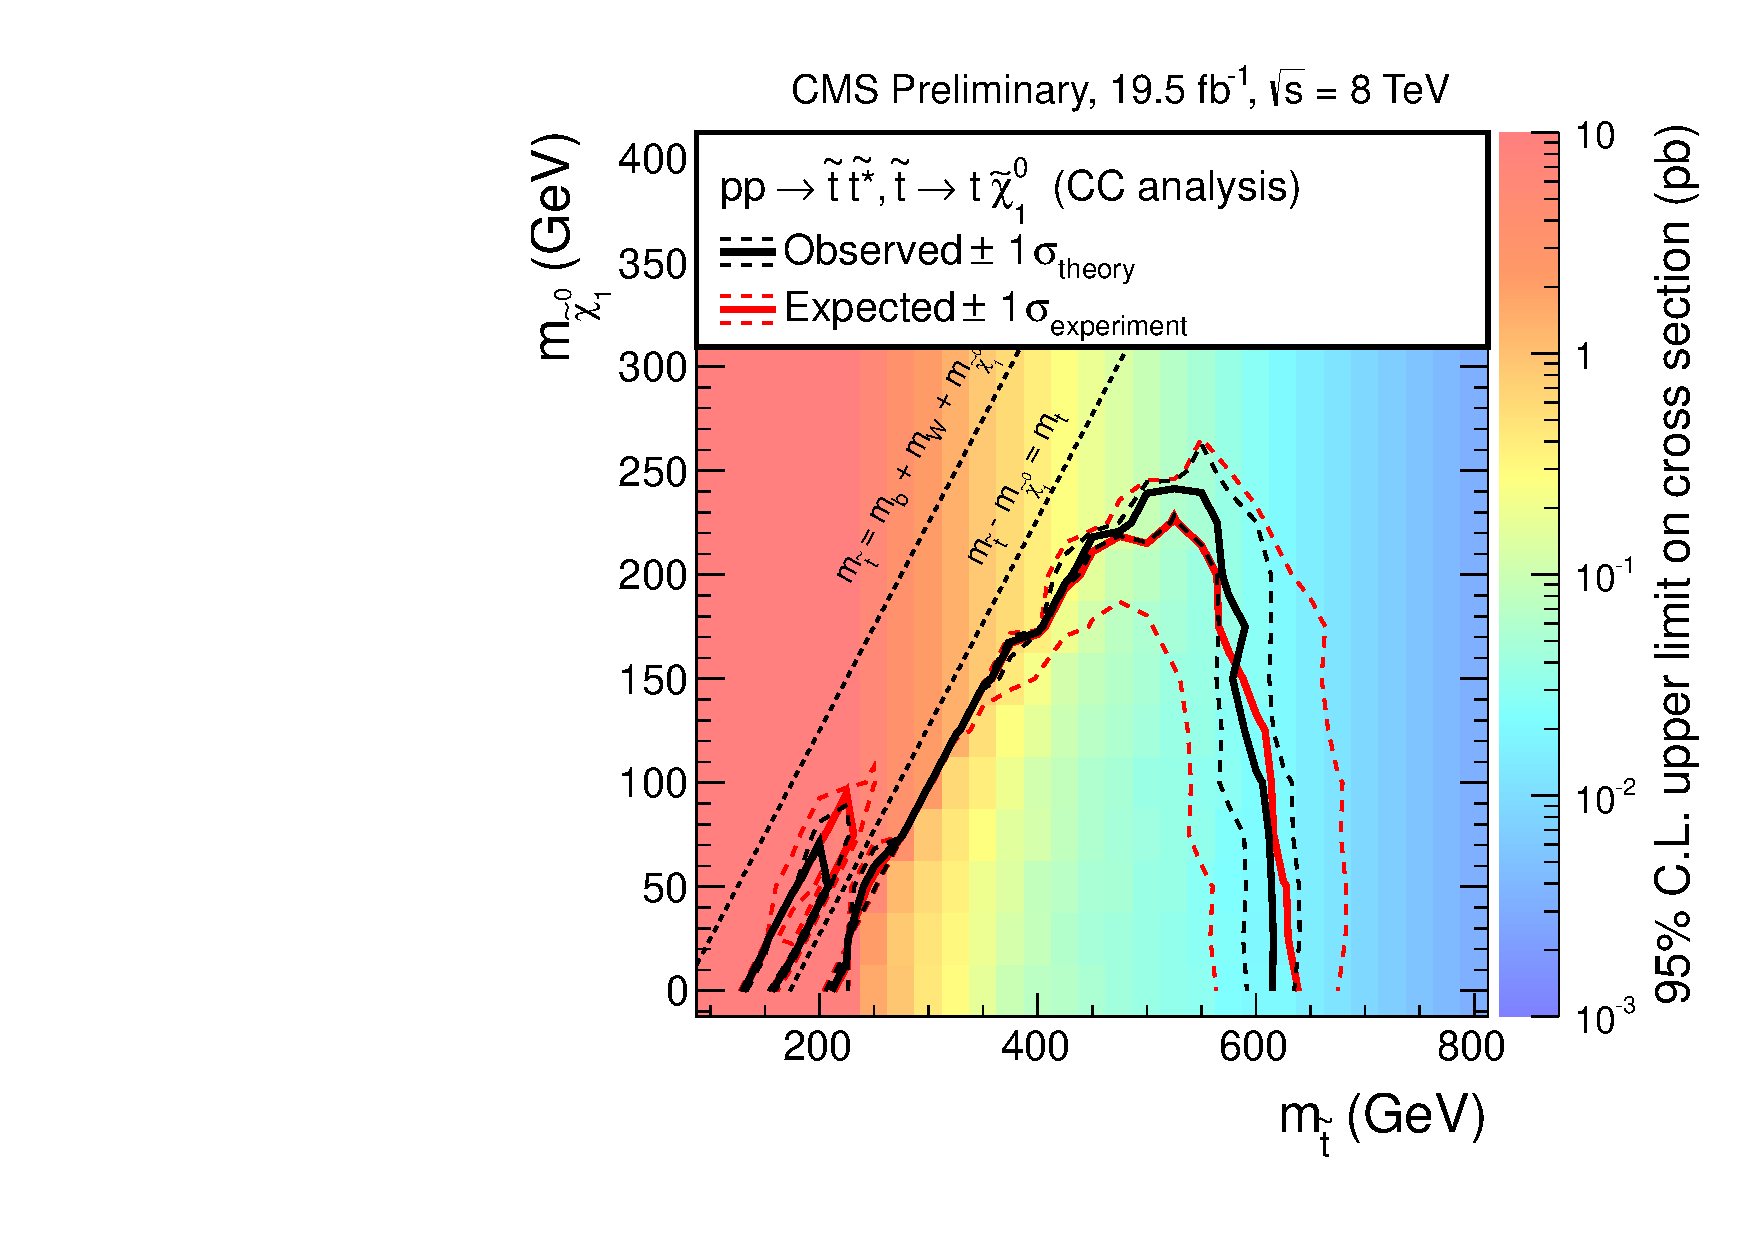
\includegraphics[width=0.31\textwidth]{limits/T2tt_CC}\\
        \includegraphics[width=0.33\textwidth]{results/CnC_T2bw075/signalRegion_MTtail_yield}
        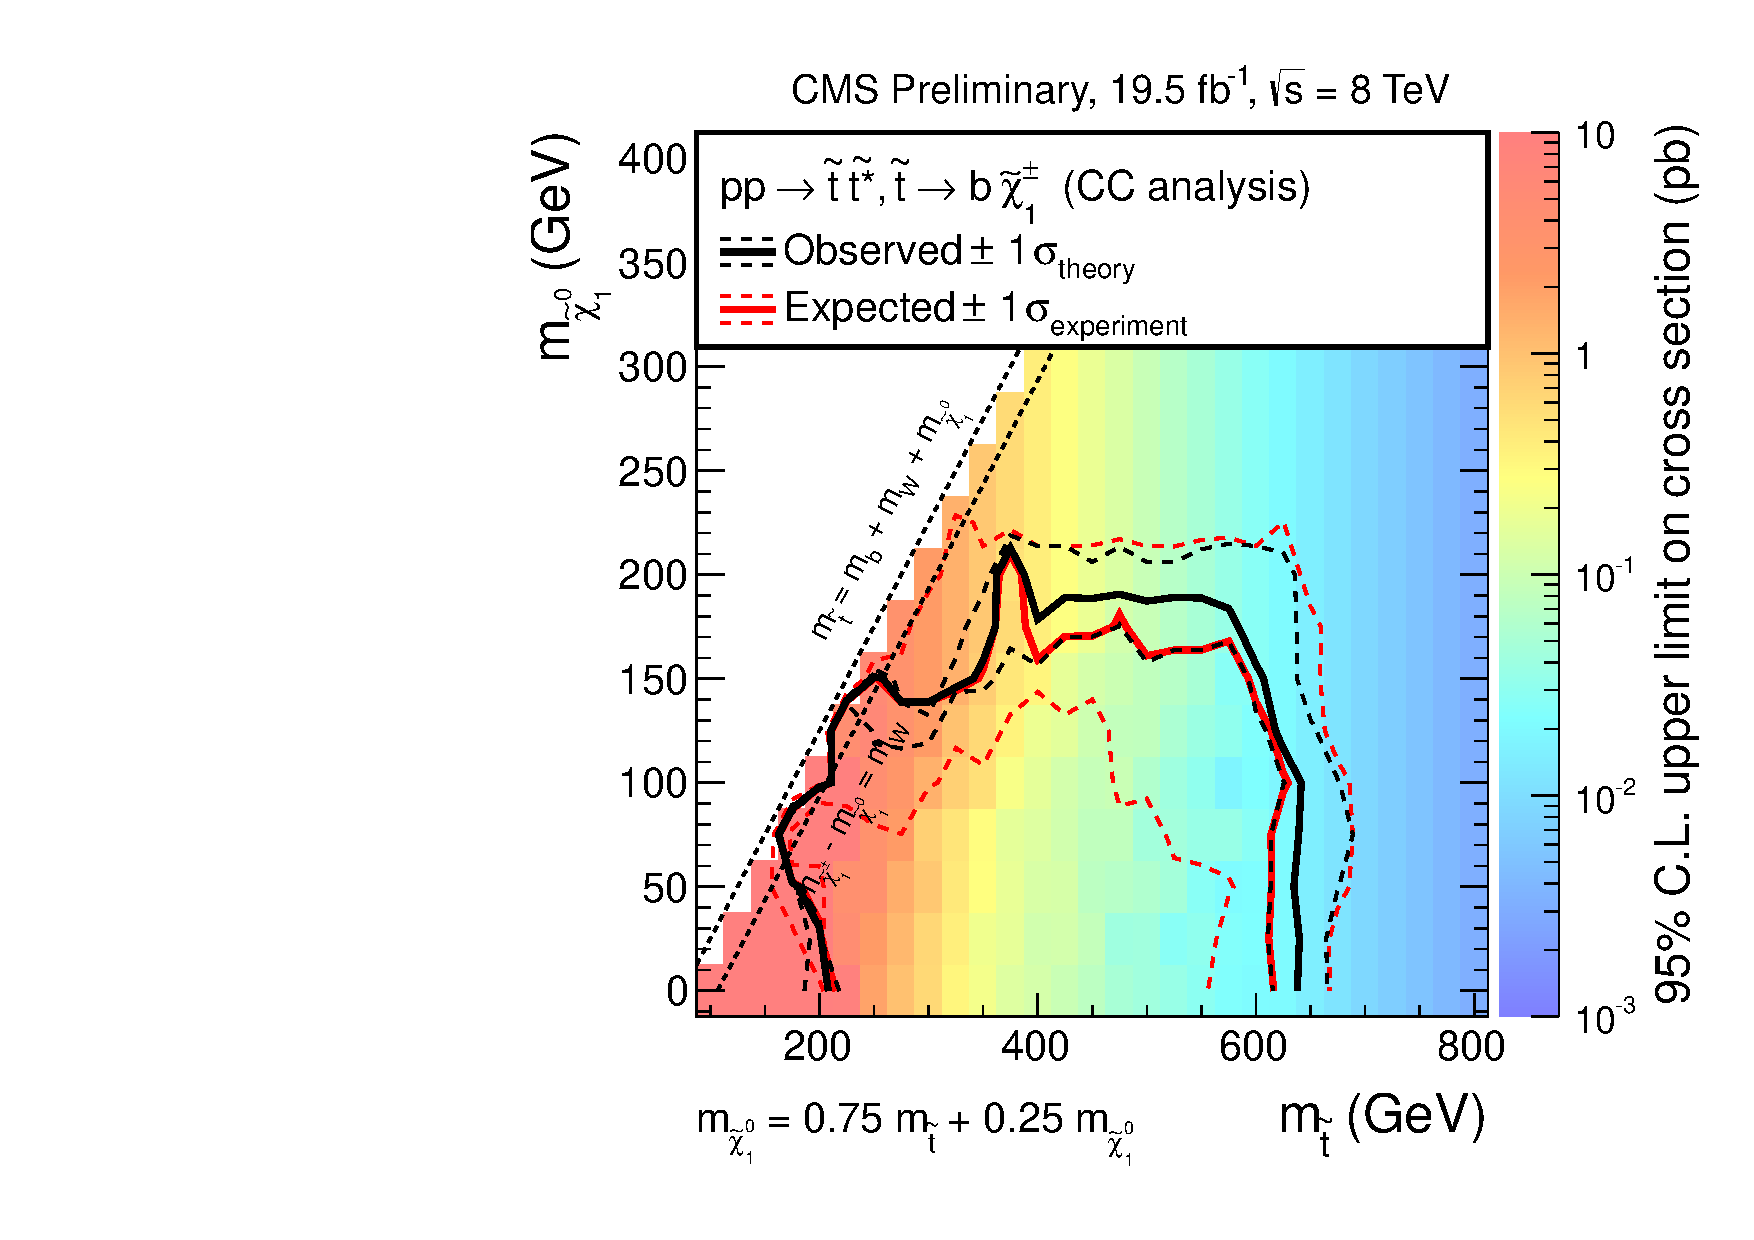
\includegraphics[width=0.31\textwidth]{limits/T2bw075_CC}\\
        \includegraphics[width=0.33\textwidth]{results/CnC_T2bw050/signalRegion_MTtail_yield}
        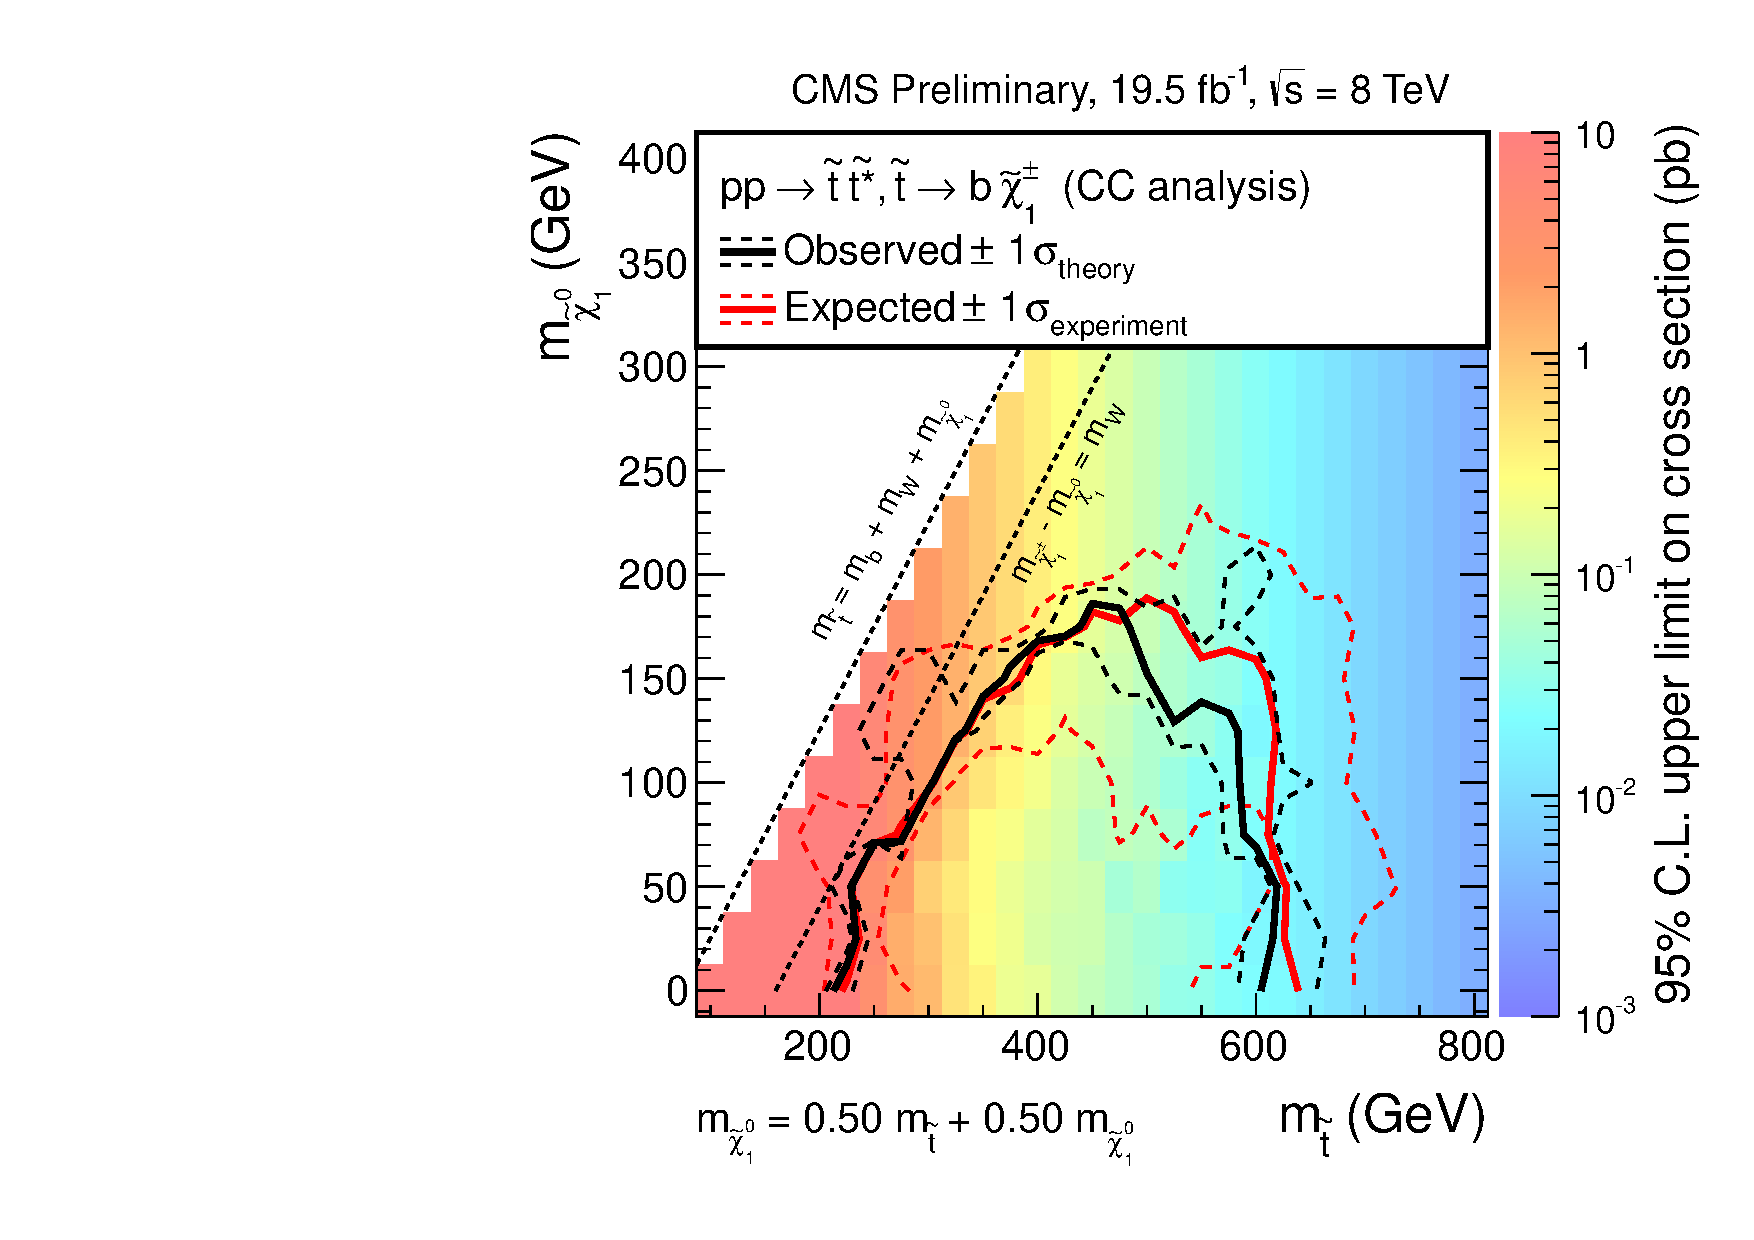
\includegraphics[width=0.31\textwidth]{limits/T2bw050_CC}\\
        \includegraphics[width=0.33\textwidth]{results/CnC_T2bw025/signalRegion_MTtail_yield}
        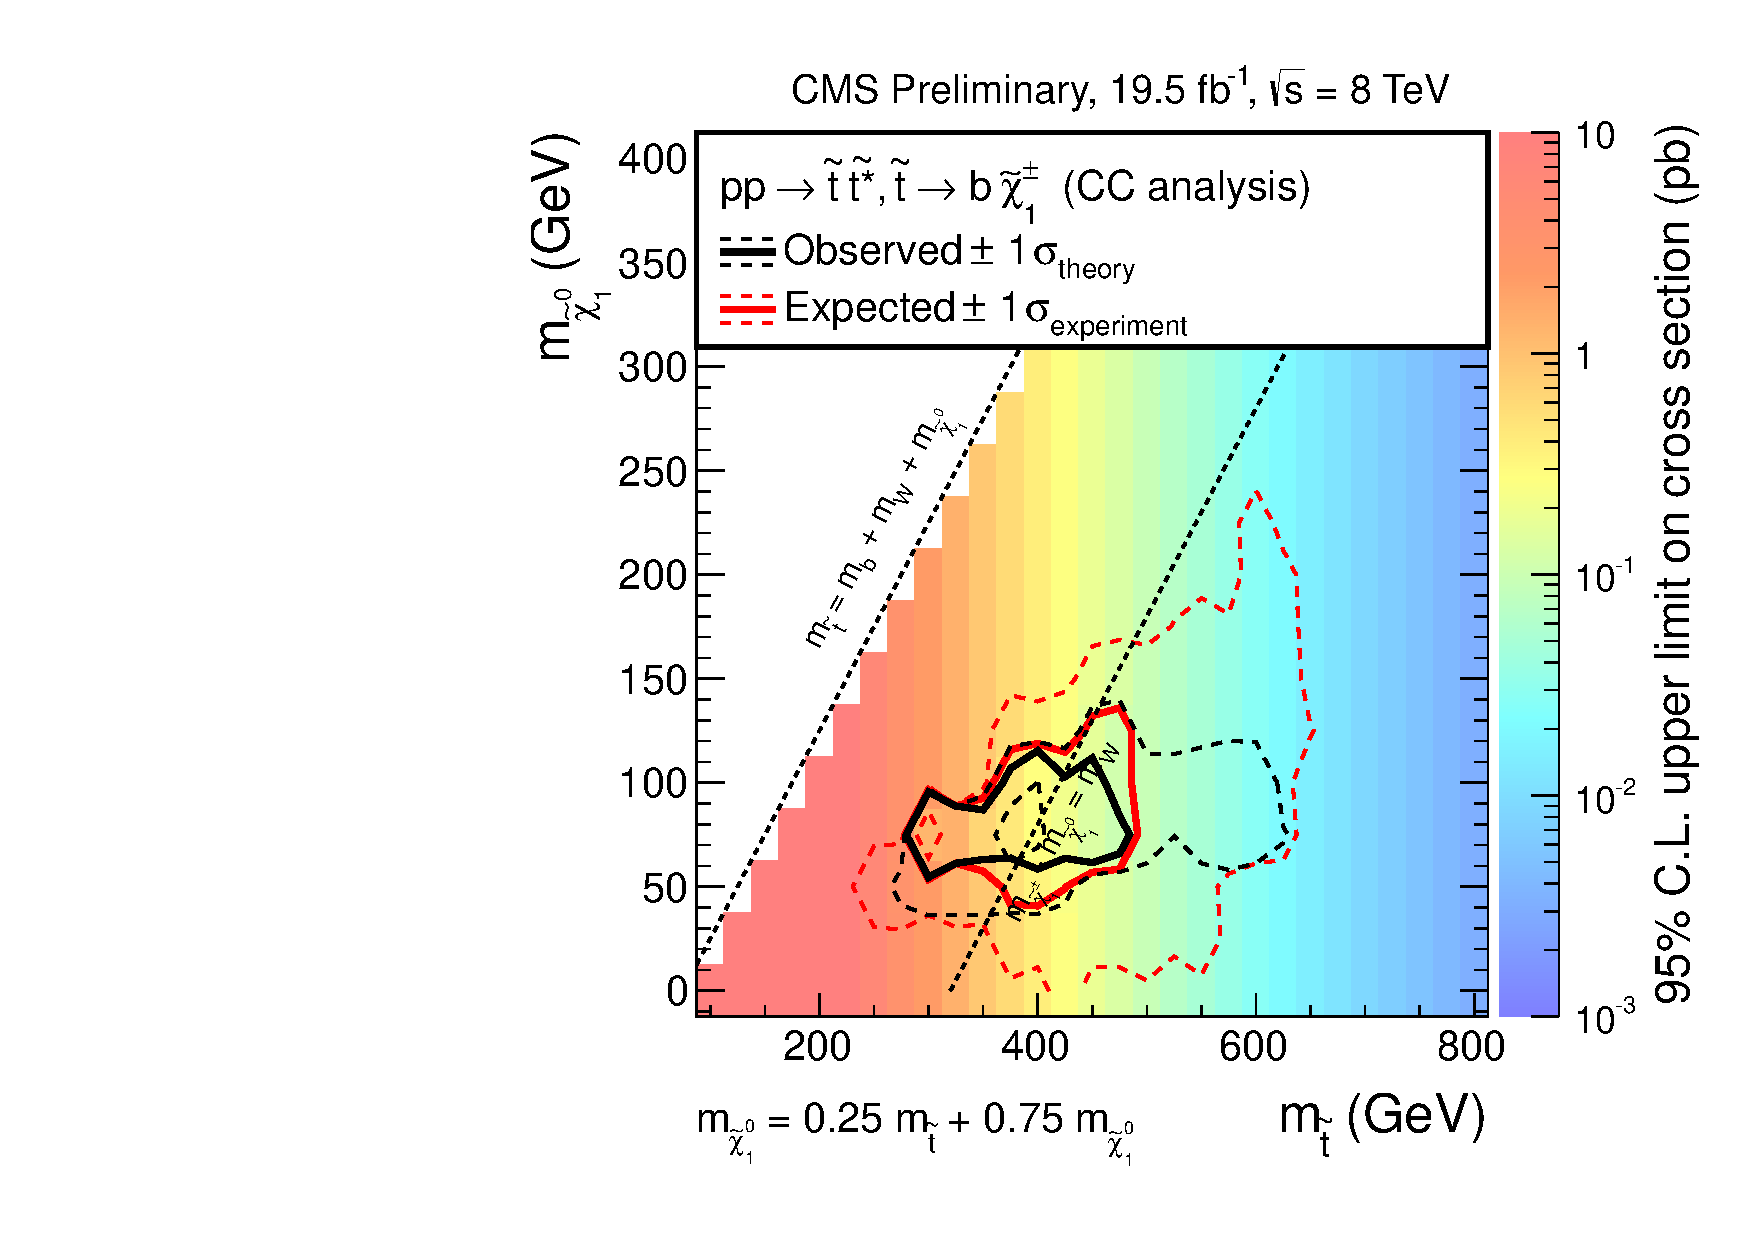
\includegraphics[width=0.31\textwidth]{limits/T2bw025_CC}\\
        \caption{On the left : comparison of the yield of the different cut-based signal
        regions between data and the background prediction under the null hypothesis. The
        grey hatching represents the systematic uncertainty, propagated on the ratio plot.
        On the right : upper limit at 95\% confidence level and exclusion in terms of
        $(\mass{\lstop},\mass{\lneutralino})$ after comparison to the theory, assuming
        $BR = 1$. On the first row, for $\lstop \rightarrow t \lneutralino$ decay mode on
        the second, third and last row for $\lstop \rightarrow b \lchargino$ decay mode
        with $x=0.75$, $0.50$ and $0.25$ respectively.}
        \label{fig:resultsCnC}
    \end{figure}

    \begin{figure}[h!]
        \centering
        \includegraphics[width=0.33\textwidth]{results/BDT_T2tt/signalRegion_MTtail_yield}
        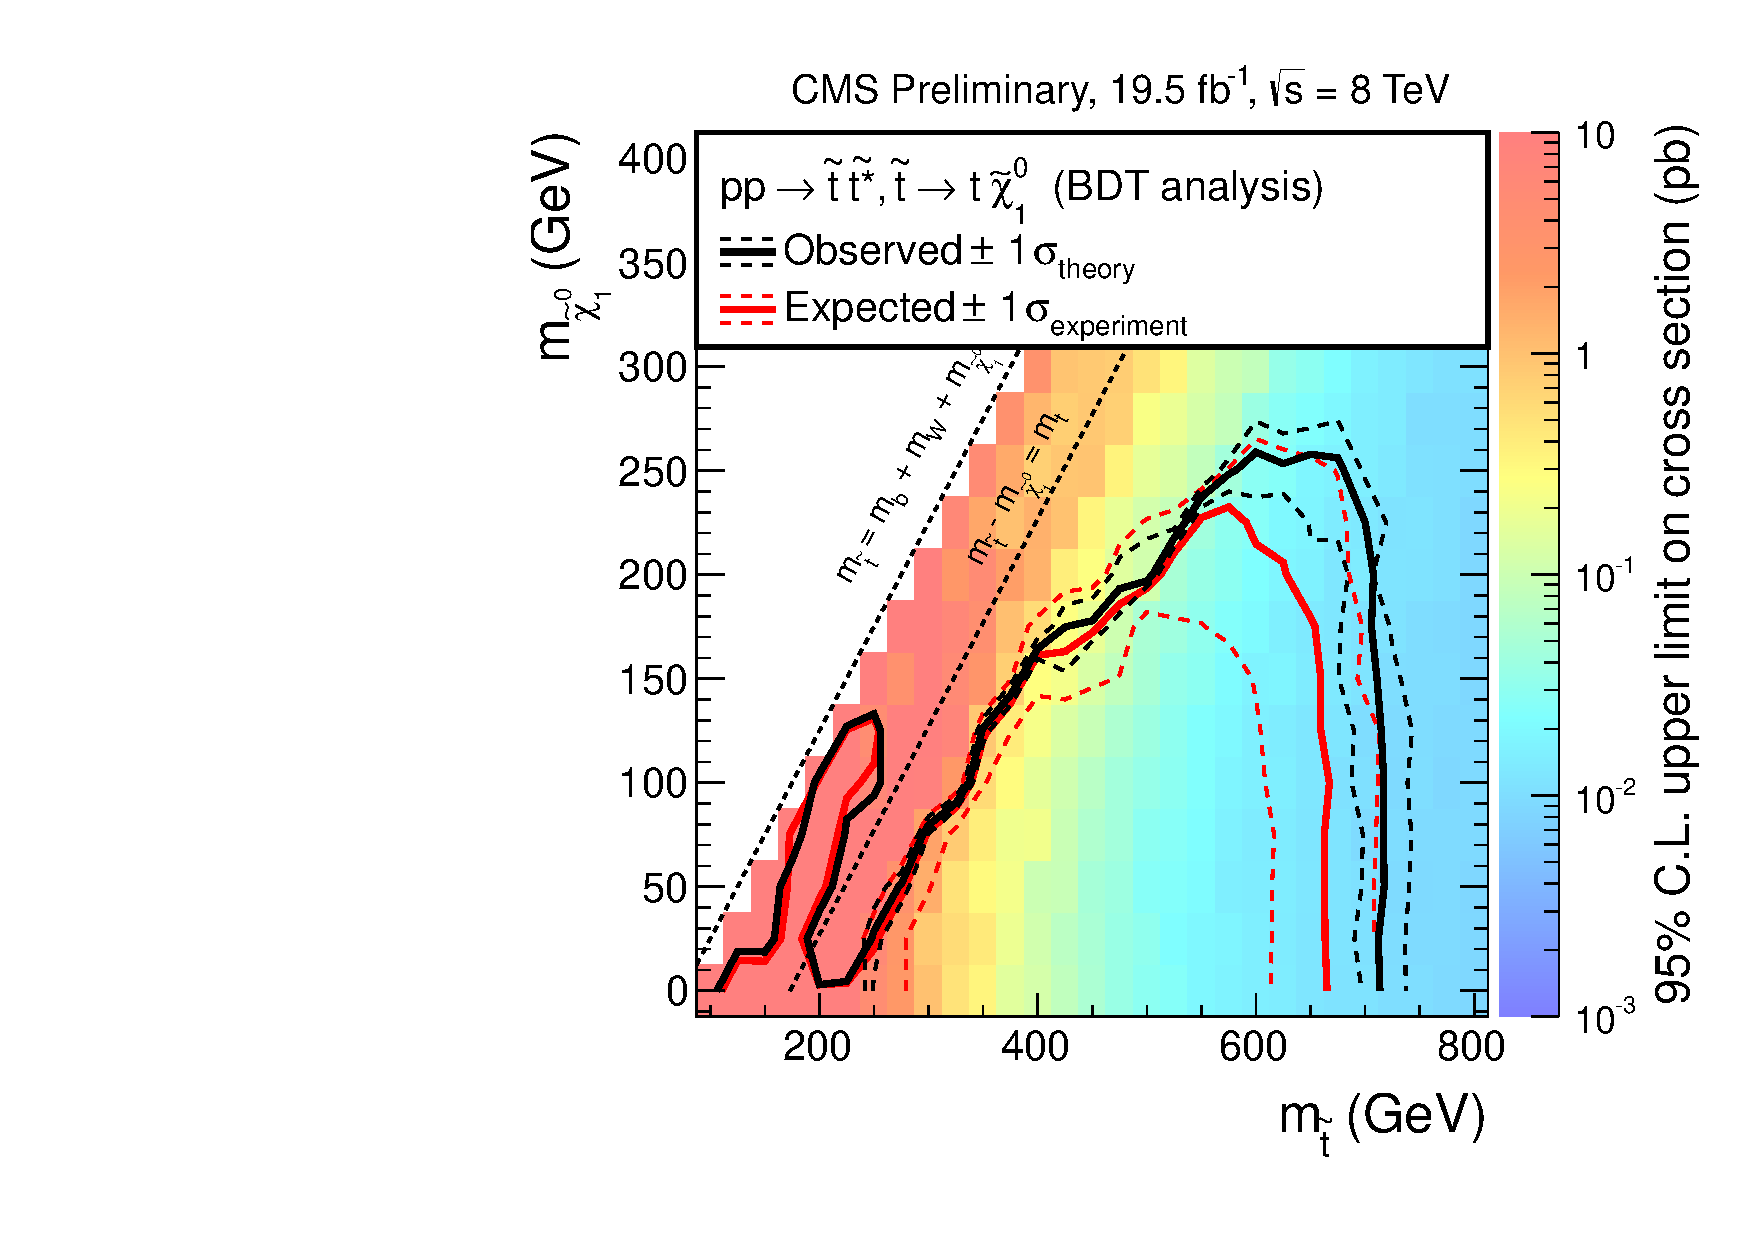
\includegraphics[width=0.31\textwidth]{limits/T2tt_BDT}\\
        \includegraphics[width=0.33\textwidth]{results/BDT_T2bw075/signalRegion_MTtail_yield}
        \includegraphics[width=0.31\textwidth]{limits/T2bw075_BDT}\\
        \includegraphics[width=0.33\textwidth]{results/BDT_T2bw050/signalRegion_MTtail_yield}
        \includegraphics[width=0.31\textwidth]{limits/T2bw050_BDT}\\
        \includegraphics[width=0.33\textwidth]{results/BDT_T2bw025/signalRegion_MTtail_yield}
        \includegraphics[width=0.31\textwidth]{limits/T2bw025_BDT}\\
        \caption{On the left : comparison of the yield of the different BDT-based signal
        regions between data and the background prediction under the null hypothesis. The
        grey hatching represents the systematic uncertainty, propagated on the ratio plot.
        On the right : upper limit at 95\% confidence level and exclusion in terms of
        $(\mass{\lstop},\mass{\lneutralino})$ after comparison to the theory, assuming
        $BR = 1$. On the first row, for $\lstop \rightarrow t \lneutralino$ decay mode on
        the second, third and last row for $\lstop \rightarrow b \lchargino$ decay mode
        with $x=0.75$, $0.50$ and $0.25$ respectively.}
        \label{fig:resultsBDT}
    \end{figure}

    The BDT approach leads to limits which are usually about $50 \GeV$ futher compared to
    the cut-based approach. For the $\lstop \rightarrow t \lneutralino$ decay mode, the
    observed exclusion using the BDT approach goes up to $\mass{\lstop} \sim 700 \GeV$
    and $\mass{\lneutralino} \sim 250 \GeV$ in the on-shell region and up to
    $\mass{\lneutralino} \sim 125 \GeV$ in the off-shell region. It is however difficult
    to exclude the region $\deltam \sim \mass{t}$ as the kinematic here is very close to
    standard model $t\bar{t}$.

    \todo{To be added when available (for the CnC especially) : polarized limits, branching
    ratio variation, maybe replace BDT results by a comparison BDT <-> CnC. \\Combination
    with 2$\ell$}

    Alternative exclusion in terms of $(\mass{\lstop}, \mass{\lneutralino})$ are proposed
    for different branching ratio assumptions, as represented on Figure \ref{fig}.
    Different polarization assumptions are also being looked at on \ref{fig:} for both
    decay types and can have a significant impact

    Figure \ref{fig:event62838873} shows one of the most signal-like event in the
    high-$\deltam$ signal region of the cut-based approach for $\lstop \rightarrow t \lneutralino$.

    \insertFigure{event62838873}{0.9}
    {One of the most signal-like event for the $\lstop \lstop^{*} \rightarrow t t \lneutralino \lneutralino$ decay-mode in the high-$\deltam$ cut-based approach. The event has one muon with $\pT = 114\GeV$, 4 jets among which 2 $b$-tag, $\MET = 392\GeV$ and $\MT = 300 \GeV$. Only tracks coming from the primary vertex are shown.}

    \newpage

    \section{Perspectives \label{sec:analysis_perspective}}
    %==============================================================

    \subsection{$W$-tagging in the high $\Delta m$ regime}

            \subsubsection{Motivation}

             As one considers higher $\Delta m$ values for the signal, the mean momentum of
             decay products increases. In particular, if we consider the hadronically
             decaying $W$, an increase of the $\pT$ translates into more colimated objects,
             in that case the pair of quarks that will hadronize. This is illustrated on
             the Figure \ref{fig:wTagging/ptW_vs_genDeltaRqq_fromttbar} showing the
             distribution of the $\Delta R$ between the
             quarks coming from the decay of a $W$ boson against the $\pT$ of the generated
             $W$. In the situation were the $\Delta R$ between the quarks approaches the
             size parameter used by the standard clustering algorithm (i.e. $\Delta R
             \sim 0.5$), only one big jet gets reconstructed instead of two smaller ones.
             This topology is refered to as boosted hadronic $W$.

             \insertFigure{wTagging/ptW_vs_genDeltaRqq_fromttbar}{0.5}{Distribution of
             the $\Delta R$ between the quarks coming from the decay of an hadronic $W$,
             as function of the generated $\pT$ of the $W$. The mean $\Delta R$ approaches
             0.5, the standard size parameter used at 8 TeV, at $\pT \sim 200\GeV$,
             meaning that jets coming from the quark will be merged by the clustering
             algorithm.}

             Driven by the fact that some new physics signatures are expected to contain
             such boosted hadronic $W$ \refNeeded, techniques have been developped to
             address this topology by providing variables to tag jets originating from
             boosted $W$ decays. The strategy consists in using a wider radius parameter
             when clustering the jets, clean and correct the jets from pile-up contamination,
             and analyze the substructure of the jets to derive variables that discriminate
             between boosted $W$ decays and fakes.

             Figure \ref{fig:} illustrate the interest that these technique might have to
             select the signal : the mean $\pT$ of the generated
             $W$ bosons for the signal accross the $(\mass{\lstop}, \mass{\lneutralino})$
             space grows as function of $\deltam$. For $\deltam > 650\GeV$, the
             mean $\pT$ is about $200\GeV$ and we can expect a large fraction of boosted $W$.
             Figure \ref{fig:} compares the distribution of the $\pT$ of the hadronic $W$ for one
             particular signal benchmark at high-$\deltam$ against the different backgrounds
             and shows that the presence a boosted $W$ tends to be discriminating.

             \insertTwoFigures{genWPtForSignal}
                              {wTagging/T2tt_meanGenWPt}{wTagging/genWPt_backgroundVsSignal}{0.4}
                              {On the left : mean $\pT$ of the generated $W$ for the
                              signal across the $(\mass{\lstop}, \mass{\lneutralino})$ space.
                              On the right : comparison of the $\pT$ spectra of the generated
                              hadronic $W$ for the $\oneLeptonTop$ and rare backgrounds and
                              the signal benchmark $(\mass{\lstop}, \mass{\lneutralino}) = (700,25) \GeV$.
                              The $\diLeptonTop$ and $\Wjets$ background are not represented
                              as they do not contain a generated hadronic $W$ by definition.}

            \subsubsection{Selection and performances}

            As an alternative to the standard anti-$k_T$ clustering algorithm with a
            size parameter $R = 0.5$ (AK5), an other jet collection is built using the
            Cambridge-Aachen clustering algorithm with a size parameter $R = 0.8$ (CA8).
            \todo{Add a reference to the detector chapter where AK, CA and kt are
            presented/compared ?}\todo{Comparison between CA and AK performances for jet
            substructure done in http://arxiv.org/pdf/0903.5081v4.pdf justifies the
            choice of CA8}

            To clean the jet from pile-up contributions and improve rejection of
            quark/gluon jets, a grooming technique called pruning is applied. It
            consists in reclustering the jet and applying
            conditions on the protojets during the algorithm, that vetos combinations of
            soft protojets with harder ones, or large angular combinations.
            \todo{Ref needed : JME-13-006, arXiv:0903.5081v4, + add sketch of grooming techniques}

            The substructure of the jet is analyzed via the $N$-subjetiness variables,
            which are designed to quantify how likely a jet is to be composed of $N$
            sub-jets. \todo{Ref to arXiv:1011.2268v3} These variables are denoted $\tau_1$,
            $\tau_2$, ... $\tau_N$. A value close to 0 for $\tau_N$ tends to indicate
            a good compatibility with the $N$-subjets hypothesis. In the context of
            $W$-tagging, it is common to focus on the use of the ratio $\tau_2/\tau_1$
            which provides good discrinability between real $W$ and quark/gluons jets.

            To define selection criteria, we study the distribution of a few variables
            on a $t\bar{t}$ Monte-Carlo sample after applying the preselection defined in
            \ref{sec:analysis_objectAndEventSelection}. We however allow events with at
            least 3 jets instead of 4. $W$ candidates are matched to generated
            hadronically-decaying $W$ : if the candidate is within $\Delta R < 0.4$, it
            is considered as matched, whereas candidates which are in $\Delta R > 2$ are
            considered to be fakes originating from quark or gluons. We studied the
            prunned mass of the jet, the $N$-subjetiness ratio $\tau_2 / \tau_1$ and the
            distance to the selected lepton $\Delta R (\ell,\text{jet})$.

            Figure \ref{fig:wTaggingVariables} shows the distribution of the prunned mass of
            the jet and the $N$-subjetiness ratio $\tau_2 / \tau_1$ for candidates with
            $\pT > 150\GeV$ and with $\Delta R(\ell,\text{jet}) > 1.5$. A good working point
            is found to be $\text{mass}(\text{jet} > 70\GeV)$ and $\tau_2 / \tau_1 < 0.5$.
            The resulting tagging efficiency is estimated as function of the $\pT$ of the
            candidate as presented on \ref{fig:wTagging/taggingEfficiency_fromttbar}.
            The efficiency for candidates matched
            to true $W$ is about 30\% at $200\GeV$ and plateau to 70\% at $270\GeV$. It
            however starts decreasing around $350\GeV$ as it gets more difficult to resolve
            the two subjets. The fake rate is about 5\% for candidates of $200\GeV$ and
            grows linearly with the $\pT$ as momentum tends to create unphysical large
            mass for the jets.

            \insertTwoFigures{wTaggingVariables}
                             {wTagging/prunnedMassAfterBasicSelection_fromttbar}
                             {wTagging/tau2OverTau1AfterBasicSelection_fromttbar}
                             {0.4}
                             {Distribution of the prunned mass (on the left) and $\tau_2
                             / \tau_1$ for CA8 jets with $\pT > 150\GeV$ and
                             $\Delta R(\ell,\text{jet}) > 1.5$ in $t\bar{t}$ events
                             with preselection applied.}

            \insertFigure{wTagging/taggingEfficiency_fromttbar}{0.5}
                         {Tagging efficiency for the true $W$ jets and fakes from quark/gluon
                         jets, as function of the $p_T$ of the jet.}

            \subsubsection{Impact on the analysis sensitivity}

            \todo{... Take one high deltamM benchmark for example, split in two channels
            0Wtag, 1Wtag. Apply standard/current selection on 0Wtag. Tune cuts for
            1Wtag. Measure sensitivity of each box+combine(need to fin how). Compare to
            current analysis with no Wtag at all. Conclude wether or not it is providing
            an increase of sensitivity. Plot as function of mStop at constant mNeutralino.}

        \subsection{Sensitivity and perspectives for the Run II}
        % =====================================================

        \loremipsum

            \subsubsection{Extrapolation of the sensitivity from Run I analysis}
        % =====================================================

        One can get a basic estimation of the integrated luminosity $\mathcal{L}$ required
        at 13 TeV to obtain equivalent sensitivity compared to 8 TeV, starting from the
        following equation :

        $$ \left( \frac{S}{\sqrt{B}} \right)_{8\TeV} = \left( \frac{S}{\sqrt{B}} \right)_{13\TeV}  $$

        Using $N = \mathcal{L} \times \sigma \times \epsilon$ and assuming that the selection
        efficiencies $\epsilon$ remain the same between $8$ and $13\TeV$, one finds that

        $$ \mathcal{L}^\text{equiv.}_{13\TeV} = \mathcal{L}_{8\TeV} \times \frac{\kappa_B}{\kappa^2_S} $$

        where $\kappa \definedAs \sigma_{13\TeV} / \sigma_{8\TeV}$. For $\mass{\lstop} \sim 800\GeV$,
        $\kappa_S \sim 10$. From the experience at $8\TeV$ using the high-$\deltam$ selection,
        the dominant backgrounds are $t\bar{t}$ and $t\bar{t}+Z$. For these processes, one
        gets $\kappa_B \sim 3.3$. One ends up with

        $$ \mathcal{L}^\text{equiv.}_{13\TeV} \sim 0.7\invfb$$

        The sensitivity has been further studied on two Monte-Carlo benchmarks for the
        $\lstop \rightarrow t \lneutralino$ signal type with $(\mass{\lstop},
        \mass{\lneutralino}) = (650,325)$ and $(850,100) \GeV$. An object selection
        strongly inspired from \ref{sec:analysis_objectAndEventSelection}, though simplified
        for this study, was used. A similar preselection is applied, requiring one electron
        or muon with $p_T > 30\GeV$, at least four jets among which one $b$-tagged, at least
        50 \GeV for $\MET$ and vetoing on a second lepton with $p_T > 5\GeV$. Table \ref{tab:phys14Preselection}
        shows the Monte-Carlo yields for $\mathcal{L} = 1\invfb$ obtained at preselection
        and after cutting on $\MT > 120\GeV$.

        \begin{table}
            \centering
                \begin{tabular}{|l|cc|}
        \hline
        &
        \textbf{preselection}   &
        \textbf{ + $M_{T}$ > 120 GeV}                                 \\
        \hline
        \textbf{$\oneLeptonTop$} & 9868  $\pm$ 18    & 614 $\pm$ 4     \\
        \textbf{$\diLeptonTop$}  & 2073  $\pm$ 8     & 1039 $\pm$ 5    \\
        \textbf{$W$+jets}        & 908   $\pm$ 74    & 55 $\pm$ 18     \\
        \textbf{rare}            & 148   $\pm$ 10    & 36 $\pm$ 3      \\
        \hline
        \textbf{total SM}        & 12998 $\pm$ 77    & 1745 $\pm$ 20   \\
        \hline
        \textbf{\textsc{T2tt} (850/100)}  & 2.57  $\pm$ 0.02  & 2.18 $\pm$ 0.02 \\
        \textbf{\textsc{T2tt} (650/325)}  & 12.11 $\pm$ 0.11  & 8.89 $\pm$ 0.09 \\
        \hline
    \end{tabular}

            \caption{\todo{To be updated with higher stat} \label{tab:phys14Preselection}}
        \end{table}

        We define three signal regions SR 1, 2 and 3 inspired from the high-$\deltam$
        selection at $8\TeV$ using only increasing cuts on $\MET$ and $\MTTwoW$ as defined
        on Table \ref{tab:phys14Cuts}. Table \ref{tab:phys14SignalREgions} shows the yield
        obtained from Monte-Carlo assuming $\mathcal{L} = 1\invfb$.

        \begin{table}
            \centering
            \begin{tabular}{c|cc}
                \textbf{Signal Region} & $E_T^\text{miss}$ & $M_{T2}^W$ \\
                \hline
                \textbf{SR1}           & >250 & >180 \\
                \textbf{SR2}           & >300 & >190 \\
                \textbf{SR3}           & >350 & >200 \\
            \end{tabular}
            \caption{\todo{Write caption} \label{tab:phys14Cuts}}
        \end{table}

        \begin{table}
            \centering
            \begin{tabular}{|l|ccc|}
\hline
&
\textbf{SR1}     &
\textbf{SR2}     &
\textbf{SR3}     \\
\hline
\textbf{$t\bar{t}$}      & 16.33 $\pm$ 7.30    & 0.00 $\pm$ 0.00    & 0.00 $\pm$ 0.00      \\
\textbf{$W$+jets}        & 0.00 $\pm$ 0.00     & 0.00 $\pm$ 0.00    & 0.00 $\pm$ 0.00      \\
\textbf{$t\bar{t}V$}     & 1.81 $\pm$ 0.09     & 1.06 $\pm$ 0.07    & 0.63 $\pm$ 0.06      \\
\hline
\textbf{total SM}        & 18.13 $\pm$ 7.30    & 1.06 $\pm$ 0.07    & 0.63 $\pm$ 0.06      \\
\hline 
\textbf{T2tt (850/100)}  & 1.41 $\pm$ 0.02     & 1.25 $\pm$ 0.02    & 1.08 $\pm$ 0.01      \\
\textbf{T2tt (650/325)}  & 2.90 $\pm$ 0.05     & 2.01 $\pm$ 0.05    & 1.27 $\pm$ 0.04      \\
\hline
\end{tabular}

            \caption{\todo{To be updated with higher stat} \label{tab:phys14SignalRegions}}
        \end{table}

       Finally, the sensitivity is estimated from the results in the SR2 region, as function
       of the integrated luminosity using $S / \sqrt{B + f^2 B^2}$ with a relative systematic
       uncertainty of $f = 50\%$ on the background. The results are presented on Figure
       \ref{fig:} and suggest that a signal with $(\mass{\lstop}, \mass{\lneutralino}) = (850,100)$
       could be excluded with $\mathcal{L} = 4\sim5\invfb$ or put in evidence with
       $\mathcal{L} = 10\sim15\invfb$.

            \insertFigure{phys14/sensitivityAsFunctionOfLumi}
                         {0.9}
                         {\todo{To be updated with higher stat (and maybe put discoverable/excluded signal strength instead ?)}}

         \subsection{Expected benefits from new object reconstruction and selection techniques}
         % =====================================================

            Techniques :
            \begin{itemize}
                \item PUPPI jets, PUPPI MET ?
                \item new isolation, ..?
                \item statistical interpretation using multiple bin to simultaneously fit S and B ? (ie simplify signal contamination treatment)
            \end{itemize}

            Variables :
            \begin{itemize}
                \item MT deconstruction, allowing to have more control to the regime looking at ? e.g. lower lepton pT  at low deltaM, more reliance on deltaPhi ?
                \item ISR tagging improvement
                \item Topness ?
                \item reduce lepton threshold ? how to probe high neutralino regime, low deltaM ?
                \item Build a 'MT significance' ?
            \end{itemize}

    \section{Overview of related searches for top partner in CMS \label{sec:analysis_overviewStopSearches}}
    %==============================================================

        \begin{itemize}
            \item Direct stop 0l (SUS-13-023)
            \item Direct stop 2l (?)
            \item Compressed spectra, monojet (SUS-13-009)

                % SUS-13-009, based on ISR, main background is Z->vv+jets and W+jets, most sensitive in low deltaM region (monojet-like events)
% the first problem is with triggering these events : the jets and leptons originating from the stop decays are too soft to be used during the online selection. The only possibility is to consider these processes with ISR with a consequent reduction in the effective cross section.

            \item Compressed spectra, soft leptons (SUS-14-021)
            \item Razor searches, gluino-mediated production ?
            \item Combinaison SUS-13-011 + Razor 0l ?? (SUS-13-011)
            \item Search for t2 -> H t1 -> ... ?
            \item Indirect searches for stealth region, using cross section measurement / spin correlation
        \end{itemize}


%==============================================================
\chapter{???}
%==============================================================
        \loremipsum


%==============================================================
\chapternonum{Conclusion}
%==============================================================
        \loremipsum





\begin{thebibliography}{2}

\addcontentsline{toc}{chapter}{Bibliography}

\singlespace

\addReference{EllisDarkMatter}
             {J. Ellis, K. A. Olive}
             {Supersymmetric Dark Matter Candidates}
             {arXiv:1001.3651}

%====================================
%Naturalness, stop motivation related
%====================================

\addReference{LEPparadox}
             {R. Barbieri, A. Strumia}
             {The `LEP paradox'}
             {arXiv:hep-ph/0007265v2}

\addReference{LectureStandardModelHiggsBoson}
             {I. van Vulpen, A. Castelli}
             {Lecture on Particle Physics II, 2011-2012, The Standard Model Higgs Boson}
             {http://master.particles.nl/LectureNotes/2011-PPII-Higgs.pdf}

%\addReference{Naturalness}
%             {S. Dimopoulos, G.F. Giudice}
%             {Naturalness Constraints in Supersymmetric Theories with Non-Universal Soft Terms.}
%             {arXiv:hep-ph/9507282}

%\addReference{}
%Baryogenesis (to read)
%http://www.slac.stanford.edu/econf/C0508141/proc/pres/ALCPG0333_TALK.PDF
%https://kicp-workshops.uchicago.edu/DM-LHC2013/depot/talk-carena-marcela.pdf
%arXiv: 1009.3969, arXiv:1110.4378,
%http://arxiv.org/pdf/1207.6330v2.pdf
%http://arxiv.org/pdf/hep-ph/0404184v1.pdf

%=================
%Simplified models
%=================

\addReference{LiemSMS}
             {S. Liem}
             {Constraining Supersymmetry using Simplified Models}
             {urn:nbn:se:su:diva-91365}

\addReference{SmodelS}
             {S. Kraml et al.}
             {SModelS: a tool for interpreting simplified-model results from the LHC and its application to supersymmetry}
             {arXiv:1312.4175v3}

%=======================
% Generator, setup
%=======================

\addReference{Powheg}
             {S. Frixione, P. Nason, C. Oleari}
             {Matching NLO QCD computations with Parton Shower simulations: the POWHEG method}
             {arXiv:0709.2092}

\addReference{Madgraph}
             {J. Alwall et al.}
             {MadGraph 5 : Going Beyond}
             {arXiv:1106.0522}

\addReference{Pythia}
             {T. Sjostrand, S. Mrenna, P. Skands}
             {Pythia 6.4 Physics and Manual}
             {arXiv:hep-ph/0603175}

%===================
% POG and PAG stuff
%===================

\addReference{METperf}
             {The CMS Collaboration}
             {Missing transverse energy performance of the CMS detector}
             {arXiv:1106.5048}

%=============
%Polarization
%=============

\addReference{polarization1}
             {M. Perelstein, A. Weiler}
             {Polarized Tops from Stop Decays at the LHC}
             {arXiv:0811.1024v2}

\addReference{polarization2}
             {Ian Low}
             {Polarized Charginos (and Tops) in Stop Decays}
             {arXiv:1304.0491v2}

%=======================
%FOM-related, statistics
%=======================

\addReference{Punzi}
             {G. Punzi}
             {Sensitivity of searches for new signals and its optimization}
             {arXiv:physics/0308063v2}

\addReference{TMVA}
             {A. Hoecker et al.}
             {TMVA - Toolkit for Multivariate Data Analysis}
             {arXiv:physics/0703039}

%========
%Analysis
%========

\addReference{SUS-12-023-PAS}
             {The CMS Collaboration}
             {Search for direct top squark pair production in events with a single isolated lepton, jets and missing transverse energy at sqrt(s) = 8 TeV}
             {CMS Physics Analysis Summary SUS-12-023}

\addReference{SUS-13-011-PUB}
             {The CMS Collaboration}
             {Search for top-squark pair production in the single-lepton final state in pp collisions at sqrt(s) = 8 TeV}
             {Eur. Phys. J. C 73 (2013) 2677. arXiv:1308.1586}

\addReference{SUS-14-015-PAS}
             {The CMS Collaboration}
             {Search for direct stop pair production in the single lepton channel at sqrt(s)=8 TeV}
             {CMS Physics Analysis Summary SUS-14-015}

%==========
%MET/sqrt(HT), MET significance
%==========

\addReference{METsignificanceMirman}
             {N. Mirman, Y. Wang, J. Alexander}
             {Missing transverse energy significance at CMS}
             {arXiv:1409.3028v1}

%========
%ISR-related
%========

\addReference{ISRtagging}
             {D. Krohn, L. Randall, L. Wang}
             {On the Feasibility and Utility of ISR Tagging}
             {arXiv:1101.0810}

\addReference{ISRGluinoTevatron}
             {J. Alwall et al.}
             {Searching for Directly Decaying Gluinos at the Tevatron}
             {arXiv:0803.0019}

\addReference{ISRmodelingDominick}
             {The CMS Collaboration}
             {Hadronic Recoil Studies of Heavy Boosted Systems}
             {CMS Analysis Note 2013/059}

%===========
%Misc / tmp
%===========

\addReference{ClosingStopGap}
             {Michal Czakon et al.}
             {Closing the stop gap}
             {arXiv:1407.1043}

\end{thebibliography}




